\documentclass[twoside]{book}

% Packages required by doxygen
\usepackage{fixltx2e}
\usepackage{calc}
\usepackage{doxygen}
\usepackage[export]{adjustbox} % also loads graphicx
\usepackage{graphicx}
\usepackage[utf8]{inputenc}
\usepackage{makeidx}
\usepackage{multicol}
\usepackage{multirow}
\PassOptionsToPackage{warn}{textcomp}
\usepackage{textcomp}
\usepackage[nointegrals]{wasysym}
\usepackage[table]{xcolor}

% Font selection
\usepackage[T1]{fontenc}
\usepackage[scaled=.90]{helvet}
\usepackage{courier}
\usepackage{amssymb}
\usepackage{sectsty}
\renewcommand{\familydefault}{\sfdefault}
\allsectionsfont{%
  \fontseries{bc}\selectfont%
  \color{darkgray}%
}
\renewcommand{\DoxyLabelFont}{%
  \fontseries{bc}\selectfont%
  \color{darkgray}%
}
\newcommand{\+}{\discretionary{\mbox{\scriptsize$\hookleftarrow$}}{}{}}

% Page & text layout
\usepackage{geometry}
\geometry{%
  a4paper,%
  top=2.5cm,%
  bottom=2.5cm,%
  left=2.5cm,%
  right=2.5cm%
}
\tolerance=750
\hfuzz=15pt
\hbadness=750
\setlength{\emergencystretch}{15pt}
\setlength{\parindent}{0cm}
\setlength{\parskip}{3ex plus 2ex minus 2ex}
\makeatletter
\renewcommand{\paragraph}{%
  \@startsection{paragraph}{4}{0ex}{-1.0ex}{1.0ex}{%
    \normalfont\normalsize\bfseries\SS@parafont%
  }%
}
\renewcommand{\subparagraph}{%
  \@startsection{subparagraph}{5}{0ex}{-1.0ex}{1.0ex}{%
    \normalfont\normalsize\bfseries\SS@subparafont%
  }%
}
\makeatother

% Headers & footers
\usepackage{fancyhdr}
\pagestyle{fancyplain}
\fancyhead[LE]{\fancyplain{}{\bfseries\thepage}}
\fancyhead[CE]{\fancyplain{}{}}
\fancyhead[RE]{\fancyplain{}{\bfseries\leftmark}}
\fancyhead[LO]{\fancyplain{}{\bfseries\rightmark}}
\fancyhead[CO]{\fancyplain{}{}}
\fancyhead[RO]{\fancyplain{}{\bfseries\thepage}}
\fancyfoot[LE]{\fancyplain{}{}}
\fancyfoot[CE]{\fancyplain{}{}}
\fancyfoot[RE]{\fancyplain{}{\bfseries\scriptsize Generated by Doxygen }}
\fancyfoot[LO]{\fancyplain{}{\bfseries\scriptsize Generated by Doxygen }}
\fancyfoot[CO]{\fancyplain{}{}}
\fancyfoot[RO]{\fancyplain{}{}}
\renewcommand{\footrulewidth}{0.4pt}
\renewcommand{\chaptermark}[1]{%
  \markboth{#1}{}%
}
\renewcommand{\sectionmark}[1]{%
  \markright{\thesection\ #1}%
}

% Indices & bibliography
\usepackage{natbib}
\usepackage[titles]{tocloft}
\setcounter{tocdepth}{3}
\setcounter{secnumdepth}{5}
\makeindex

% Hyperlinks (required, but should be loaded last)
\usepackage{ifpdf}
\ifpdf
  \usepackage[pdftex,pagebackref=true]{hyperref}
\else
  \usepackage[ps2pdf,pagebackref=true]{hyperref}
\fi
\hypersetup{%
  colorlinks=true,%
  linkcolor=blue,%
  citecolor=blue,%
  unicode%
}

% Custom commands
\newcommand{\clearemptydoublepage}{%
  \newpage{\pagestyle{empty}\cleardoublepage}%
}

\usepackage{caption}
\captionsetup{labelsep=space,justification=centering,font={bf},singlelinecheck=off,skip=4pt,position=top}

%===== C O N T E N T S =====

\begin{document}

% Titlepage & ToC
\hypersetup{pageanchor=false,
             bookmarksnumbered=true,
             pdfencoding=unicode
            }
\pagenumbering{roman}
\begin{titlepage}
\vspace*{7cm}
\begin{center}%
{\Large V\+PL }\\
\vspace*{1cm}
{\large Generated by Doxygen 1.8.11}\\
\end{center}
\end{titlepage}
\clearemptydoublepage
\tableofcontents
\clearemptydoublepage
\pagenumbering{arabic}
\hypersetup{pageanchor=true}

%--- Begin generated contents ---
\chapter{View Planning Library}
\label{index}\hypertarget{index}{}\begin{quote}
Consejo Nacional de Ciencia y Tecnología (C\+O\+N\+A\+CyT) \end{quote}


\begin{quote}
Instituto Nacional de Astrofísica Óptica y Electrónica (I\+N\+A\+OE). \end{quote}


\begin{quote}
Centro de Innovación y Desarrollo Tecnológico (I\+P\+N-\/\+C\+I\+D\+E\+T\+EC). \end{quote}


V\+P\+L(\+The acronym of view planning library) provides a platform to develop view planning algorithms and perform comparisons quickly. V\+PL is written in C++ and it is based on a set of well known libraries\+: octomap and M\+R\+PT. V\+PL provides the data structures to represent the space, provides visibility algorithms, implements several view planning algorithms reported in the literature and provides flexibility to link with range sensor simulators and motion planning algorithms. V\+PL was developed by \href{https://jivasquez.wordpress.com}{\tt J. Irving Vasquez-\/\+Gomez} under New B\+SD license.

V\+PL is composed of two main modules\+: Partial\+Model and View\+Planning. Partial\+Model stores the information about object that is being reconstructed and provides a set of functions to handle visibility for next best view calculation. View\+Planning provides planning algorithms to achieve an automated reconstruction. Additional modules are included but they can be ommited during compilation\+: rangesimulator and nbvs planning.



More information is in our \href{https://jivasquez.files.wordpress.com/2017/05/vas_vpl_towards.pdf}{\tt V\+PL paper} currently under development.

If your are using V\+PL in an academy work please cite (so far)\+:

Vasquez-\/\+Gomez, J. I., Sucar, L. E., \& Murrieta-\/\+Cid, R. (2017). View/state planning for three-\/dimensional object reconstruction under uncertainty. Autonomous Robots, 41(1), 89-\/109.


\begin{DoxyCode}
1 @article\{vasquez2017view,
2   title=\{View/state planning for three-dimensional object reconstruction under uncertainty\},
3   author=\{Vasquez-Gomez, J Irving and Sucar, L Enrique and Murrieta-Cid, Rafael\},
4   journal=\{Autonomous Robots\},
5   volume=\{41\},
6   number=\{1\},
7   pages=\{89--109\},
8   year=\{2017\},
9   publisher=\{Springer\}
10 \}
\end{DoxyCode}
 If you are having troubles with V\+PL, please drop me a mail\+: 

\subsubsection*{Pre-\/processing the input files}


\begin{DoxyItemize}
\item File {\ttfamily cloud\+\_\+generation.\+py} (inside pre-\/processing folder) generates the point clouds needed in vpl files. In folder {\ttfamily input\+\_\+dataset\+\_\+folder} the folder where Hintertoisser dataset files are stored is indicated. And {\ttfamily output\+\_\+dataset\+\_\+folder} indicates the location where we will save the output point clouds.
\item File {\ttfamily scaling.\+py} scales the input point cloud of the ground truth model.
\end{DoxyItemize}

\subsubsection*{Requirements}

Before installing V\+PL you need to install the following libraries\+:
\begin{DoxyItemize}
\item boost 
\begin{DoxyCode}
1 sudo apt get install libboost-all-dev
\end{DoxyCode}

\item \href{https://octomap.github.io/>}{\tt octomap} 
\begin{DoxyCode}
1 git clone https://github.com/OctoMap/octomap.git
\end{DoxyCode}

\item \href{http://www.mrpt.org/>}{\tt M\+R\+PT} I installed it from Ubuntu P\+PA
\end{DoxyItemize}

\subsubsection*{Installation}


\begin{DoxyEnumerate}
\item Download and install \href{https://octomap.github.io/>}{\tt octomap} and \href{http://www.mrpt.org/>}{\tt M\+R\+PT}. M\+R\+PT was installed from source not P\+PA
\item Clone this repo to your machine 
\begin{DoxyCode}
1 git clone https://github.com/irvingvasquez/vpl
\end{DoxyCode}

\item Configure the C\+Make\+Lists.\+txt at top file
\item Compile the library. Move to the V\+PL top folder and run\+: 
\begin{DoxyCode}
1 mkdir build
2 cd build 
3 cmake ..
\end{DoxyCode}

\end{DoxyEnumerate}

\subsubsection*{Full V\+PL installation}

we recommend that V\+PL will be installed in the same folder that the required libraries\+:


\begin{DoxyItemize}
\item octomap-\/devel
\end{DoxyItemize}

To compile the library move to the V\+PL top folder and run\+:


\begin{DoxyCode}
1 cd VPL
2 mkdir build
3 cd build    
4 cmake ..
\end{DoxyCode}
 {\ttfamily Note\+:if you are using your custom folder hierarchy you should modify the C\+Make\+Lists.\+txt in order to match the folders} 
\chapter{Hierarchical Index}
\section{Class Hierarchy}
This inheritance list is sorted roughly, but not completely, alphabetically\+:\begin{DoxyCompactList}
\item Color\+Oc\+Tree\begin{DoxyCompactList}
\item \contentsline{section}{C\+Octree\+V\+PL}{\pageref{classCOctreeVPL}}{}
\begin{DoxyCompactList}
\item \contentsline{section}{C\+Octree\+Kriegel12}{\pageref{classCOctreeKriegel12}}{}
\item \contentsline{section}{C\+Octree\+Occussion\+Aware}{\pageref{classCOctreeOccussionAware}}{}
\item \contentsline{section}{C\+Octree\+Rear\+Side\+Voxel}{\pageref{classCOctreeRearSideVoxel}}{}
\end{DoxyCompactList}
\end{DoxyCompactList}
\item \contentsline{section}{Evaluation\+Result}{\pageref{classEvaluationResult}}{}
\item \contentsline{section}{I\+N\+I\+Reader}{\pageref{classINIReader}}{}
\item list\begin{DoxyCompactList}
\item \contentsline{section}{View\+List}{\pageref{classViewList}}{}
\item \contentsline{section}{vp\+Triangle\+List}{\pageref{classvpTriangleList}}{}
\end{DoxyCompactList}
\item \contentsline{section}{N\+B\+V\+Planner}{\pageref{classNBVPlanner}}{}
\begin{DoxyCompactList}
\item \contentsline{section}{Workspace\+N\+B\+V\+Planner}{\pageref{classWorkspaceNBVPlanner}}{}
\begin{DoxyCompactList}
\item \contentsline{section}{Training\+Planner}{\pageref{classTrainingPlanner}}{}
\end{DoxyCompactList}
\end{DoxyCompactList}
\item \contentsline{section}{Partial\+Model\+Base}{\pageref{classPartialModelBase}}{}
\begin{DoxyCompactList}
\item \contentsline{section}{P\+M\+Volumetric}{\pageref{classPMVolumetric}}{}
\begin{DoxyCompactList}
\item \contentsline{section}{P\+M\+V\+Octree}{\pageref{classPMVOctree}}{}
\begin{DoxyCompactList}
\item \contentsline{section}{P\+M\+V\+Octree\+IG}{\pageref{classPMVOctreeIG}}{}
\item \contentsline{section}{P\+M\+V\+Octree\+I\+G\+Kriegel12}{\pageref{classPMVOctreeIGKriegel12}}{}
\item \contentsline{section}{P\+M\+V\+Octree\+Occusion\+Aware}{\pageref{classPMVOctreeOccusionAware}}{}
\item \contentsline{section}{P\+M\+V\+Octree\+Vasquez09}{\pageref{classPMVOctreeVasquez09}}{}
\item \contentsline{section}{P\+M\+V\+Octree\+Volume}{\pageref{classPMVOctreeVolume}}{}
\item \contentsline{section}{P\+M\+V\+O\+Rear\+Side\+Voxel}{\pageref{classPMVORearSideVoxel}}{}
\end{DoxyCompactList}
\end{DoxyCompactList}
\end{DoxyCompactList}
\item \contentsline{section}{Range\+Sensor}{\pageref{classRangeSensor}}{}
\item \contentsline{section}{Reconstructor3D}{\pageref{classReconstructor3D}}{}
\begin{DoxyCompactList}
\item \contentsline{section}{R3\+D\+Direct\+Positioning}{\pageref{classR3DDirectPositioning}}{}
\begin{DoxyCompactList}
\item \contentsline{section}{Reconstructor3\+D\+Exp\+Utility}{\pageref{classReconstructor3DExpUtility}}{}
\end{DoxyCompactList}
\item \contentsline{section}{Reconstructor3\+D\+Robot}{\pageref{classReconstructor3DRobot}}{}
\end{DoxyCompactList}
\item \contentsline{section}{Robot\+Sensor}{\pageref{classRobotSensor}}{}
\begin{DoxyCompactList}
\item \contentsline{section}{Rob\+Sen\+No\+Transformation}{\pageref{classRobSenNoTransformation}}{}
\end{DoxyCompactList}
\item vector\begin{DoxyCompactList}
\item \contentsline{section}{Evaluation\+Result\+Vector}{\pageref{classEvaluationResultVector}}{}
\end{DoxyCompactList}
\item \contentsline{section}{View\+Structure}{\pageref{classViewStructure}}{}
\item \contentsline{section}{View\+Synthesis}{\pageref{classViewSynthesis}}{}
\begin{DoxyCompactList}
\item \contentsline{section}{Random\+View\+Synthesis}{\pageref{classRandomViewSynthesis}}{}
\item \contentsline{section}{View\+Sphere\+Synthesis}{\pageref{classViewSphereSynthesis}}{}
\end{DoxyCompactList}
\item \contentsline{section}{vp\+File\+Reader}{\pageref{classvpFileReader}}{}
\item \contentsline{section}{vp\+Robot}{\pageref{classvpRobot}}{}
\begin{DoxyCompactList}
\item \contentsline{section}{vpr\+Free\+Flyer}{\pageref{classvprFreeFlyer}}{}
\end{DoxyCompactList}
\item \contentsline{section}{vp\+Triangle}{\pageref{classvpTriangle}}{}
\item \contentsline{section}{vp\+Vertex}{\pageref{classvpVertex}}{}
\end{DoxyCompactList}

\chapter{Class Index}
\section{Class List}
Here are the classes, structs, unions and interfaces with brief descriptions\+:\begin{DoxyCompactList}
\item\contentsline{section}{\hyperlink{classCOctreeKriegel12}{C\+Octree\+Kriegel12} }{\pageref{classCOctreeKriegel12}}{}
\item\contentsline{section}{\hyperlink{classCOctreeOccussionAware}{C\+Octree\+Occussion\+Aware} }{\pageref{classCOctreeOccussionAware}}{}
\item\contentsline{section}{\hyperlink{classCOctreeRearSideVoxel}{C\+Octree\+Rear\+Side\+Voxel} }{\pageref{classCOctreeRearSideVoxel}}{}
\item\contentsline{section}{\hyperlink{classCOctreeVPL}{C\+Octree\+V\+PL} }{\pageref{classCOctreeVPL}}{}
\item\contentsline{section}{\hyperlink{classEvaluationResult}{Evaluation\+Result} }{\pageref{classEvaluationResult}}{}
\item\contentsline{section}{\hyperlink{classEvaluationResultVector}{Evaluation\+Result\+Vector} }{\pageref{classEvaluationResultVector}}{}
\item\contentsline{section}{\hyperlink{classINIReader}{I\+N\+I\+Reader} }{\pageref{classINIReader}}{}
\item\contentsline{section}{\hyperlink{classNBVPlanner}{N\+B\+V\+Planner} }{\pageref{classNBVPlanner}}{}
\item\contentsline{section}{\hyperlink{classPartialModelBase}{Partial\+Model\+Base} }{\pageref{classPartialModelBase}}{}
\item\contentsline{section}{\hyperlink{classPMVOctree}{P\+M\+V\+Octree} }{\pageref{classPMVOctree}}{}
\item\contentsline{section}{\hyperlink{classPMVOctreeIG}{P\+M\+V\+Octree\+IG} }{\pageref{classPMVOctreeIG}}{}
\item\contentsline{section}{\hyperlink{classPMVOctreeIGKriegel12}{P\+M\+V\+Octree\+I\+G\+Kriegel12} }{\pageref{classPMVOctreeIGKriegel12}}{}
\item\contentsline{section}{\hyperlink{classPMVOctreeOccusionAware}{P\+M\+V\+Octree\+Occusion\+Aware} }{\pageref{classPMVOctreeOccusionAware}}{}
\item\contentsline{section}{\hyperlink{classPMVOctreeVasquez09}{P\+M\+V\+Octree\+Vasquez09} }{\pageref{classPMVOctreeVasquez09}}{}
\item\contentsline{section}{\hyperlink{classPMVOctreeVolume}{P\+M\+V\+Octree\+Volume} }{\pageref{classPMVOctreeVolume}}{}
\item\contentsline{section}{\hyperlink{classPMVolumetric}{P\+M\+Volumetric} }{\pageref{classPMVolumetric}}{}
\item\contentsline{section}{\hyperlink{classPMVORearSideVoxel}{P\+M\+V\+O\+Rear\+Side\+Voxel} }{\pageref{classPMVORearSideVoxel}}{}
\item\contentsline{section}{\hyperlink{classR3DDirectPositioning}{R3\+D\+Direct\+Positioning} }{\pageref{classR3DDirectPositioning}}{}
\item\contentsline{section}{\hyperlink{classRandomViewSynthesis}{Random\+View\+Synthesis} }{\pageref{classRandomViewSynthesis}}{}
\item\contentsline{section}{\hyperlink{classRangeSensor}{Range\+Sensor} }{\pageref{classRangeSensor}}{}
\item\contentsline{section}{\hyperlink{classReconstructor3D}{Reconstructor3D} }{\pageref{classReconstructor3D}}{}
\item\contentsline{section}{\hyperlink{classReconstructor3DExpUtility}{Reconstructor3\+D\+Exp\+Utility} }{\pageref{classReconstructor3DExpUtility}}{}
\item\contentsline{section}{\hyperlink{classReconstructor3DRobot}{Reconstructor3\+D\+Robot} }{\pageref{classReconstructor3DRobot}}{}
\item\contentsline{section}{\hyperlink{classRobotSensor}{Robot\+Sensor} }{\pageref{classRobotSensor}}{}
\item\contentsline{section}{\hyperlink{classRobSenNoTransformation}{Rob\+Sen\+No\+Transformation} }{\pageref{classRobSenNoTransformation}}{}
\item\contentsline{section}{\hyperlink{classViewList}{View\+List} }{\pageref{classViewList}}{}
\item\contentsline{section}{\hyperlink{classViewSphereSynthesis}{View\+Sphere\+Synthesis} }{\pageref{classViewSphereSynthesis}}{}
\item\contentsline{section}{\hyperlink{classViewStructure}{View\+Structure} }{\pageref{classViewStructure}}{}
\item\contentsline{section}{\hyperlink{classViewSynthesis}{View\+Synthesis} }{\pageref{classViewSynthesis}}{}
\item\contentsline{section}{\hyperlink{classvpFileReader}{vp\+File\+Reader} }{\pageref{classvpFileReader}}{}
\item\contentsline{section}{\hyperlink{classvprFreeFlyer}{vpr\+Free\+Flyer} }{\pageref{classvprFreeFlyer}}{}
\item\contentsline{section}{\hyperlink{classvpRobot}{vp\+Robot} }{\pageref{classvpRobot}}{}
\item\contentsline{section}{\hyperlink{classvpTriangle}{vp\+Triangle} }{\pageref{classvpTriangle}}{}
\item\contentsline{section}{\hyperlink{classvpTriangleList}{vp\+Triangle\+List} }{\pageref{classvpTriangleList}}{}
\item\contentsline{section}{\hyperlink{classvpVertex}{vp\+Vertex} }{\pageref{classvpVertex}}{}
\item\contentsline{section}{\hyperlink{classWorkspaceNBVPlanner}{Workspace\+N\+B\+V\+Planner} }{\pageref{classWorkspaceNBVPlanner}}{}
\end{DoxyCompactList}

\chapter{Class Documentation}
\hypertarget{classCOctreeKriegel12}{}\section{C\+Octree\+Kriegel12 Class Reference}
\label{classCOctreeKriegel12}\index{C\+Octree\+Kriegel12@{C\+Octree\+Kriegel12}}


{\ttfamily \#include $<$pmvoctreeigkriegel12.\+h$>$}

Inheritance diagram for C\+Octree\+Kriegel12\+:\begin{figure}[H]
\begin{center}
\leavevmode
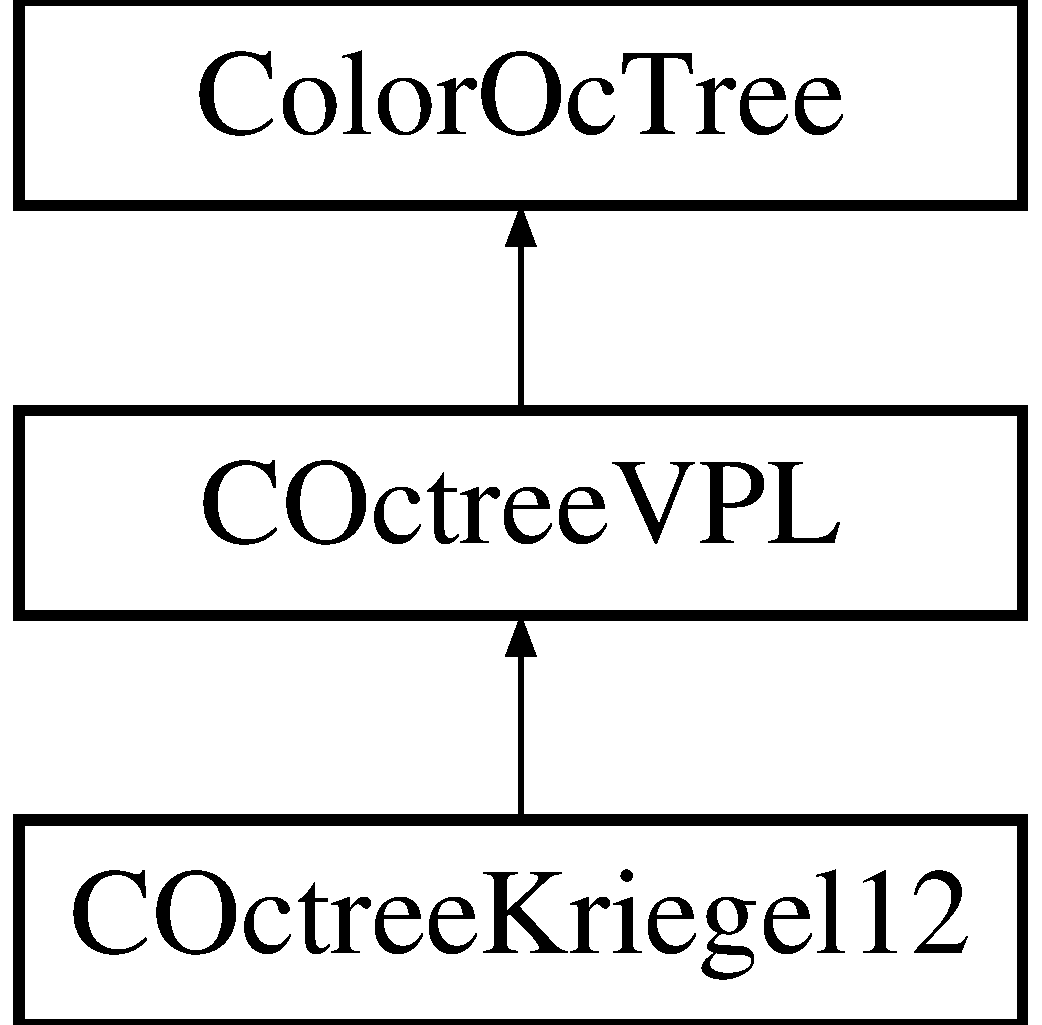
\includegraphics[height=3.000000cm]{classCOctreeKriegel12}
\end{center}
\end{figure}
\subsection*{Public Member Functions}
\begin{DoxyCompactItemize}
\item 
{\bfseries C\+Octree\+Kriegel12} (double resolution)\hypertarget{classCOctreeKriegel12_a5869334baea8686aff6f87df14676d07}{}\label{classCOctreeKriegel12_a5869334baea8686aff6f87df14676d07}

\item 
virtual double \hyperlink{classCOctreeKriegel12_aa900e135c79350675fb0b6a9ab5e3c02}{cast\+Ray\+IG} (const point3d \&origin, const point3d \&directionP, point3d \&end, bool ignore\+Unknown\+Cells=false, double max\+Range=-\/1.\+0)
\end{DoxyCompactItemize}
\subsection*{Additional Inherited Members}


\subsection{Detailed Description}
Implementation status\+: ok Testing status\+: ok 

\subsection{Member Function Documentation}
\index{C\+Octree\+Kriegel12@{C\+Octree\+Kriegel12}!cast\+Ray\+IG@{cast\+Ray\+IG}}
\index{cast\+Ray\+IG@{cast\+Ray\+IG}!C\+Octree\+Kriegel12@{C\+Octree\+Kriegel12}}
\subsubsection[{\texorpdfstring{cast\+Ray\+I\+G(const point3d \&origin, const point3d \&direction\+P, point3d \&end, bool ignore\+Unknown\+Cells=false, double max\+Range=-\/1.\+0)}{castRayIG(const point3d &origin, const point3d &directionP, point3d &end, bool ignoreUnknownCells=false, double maxRange=-1.0)}}]{\setlength{\rightskip}{0pt plus 5cm}double C\+Octree\+Kriegel12\+::cast\+Ray\+IG (
\begin{DoxyParamCaption}
\item[{const point3d \&}]{origin, }
\item[{const point3d \&}]{directionP, }
\item[{point3d \&}]{end, }
\item[{bool}]{ignore\+Unknown\+Cells = {\ttfamily false}, }
\item[{double}]{max\+Range = {\ttfamily -\/1.0}}
\end{DoxyParamCaption}
)\hspace{0.3cm}{\ttfamily [virtual]}}\hypertarget{classCOctreeKriegel12_aa900e135c79350675fb0b6a9ab5e3c02}{}\label{classCOctreeKriegel12_aa900e135c79350675fb0b6a9ab5e3c02}
Traces a Ray and returns the information gain of a ray. Integrates even for already touched voxels. Kriegel 12 cast\+Ray Information Gain !!!!! 

Reimplemented from \hyperlink{classCOctreeVPL_a3a13d4e2bf90156a0bcc672feb2d521f}{C\+Octree\+V\+PL}.



The documentation for this class was generated from the following files\+:\begin{DoxyCompactItemize}
\item 
partialmodel/pmvoctreeigkriegel12.\+h\item 
partialmodel/pmvoctreeigkriegel12.\+cpp\end{DoxyCompactItemize}

\hypertarget{classCOctreeOccussionAware}{}\section{C\+Octree\+Occussion\+Aware Class Reference}
\label{classCOctreeOccussionAware}\index{C\+Octree\+Occussion\+Aware@{C\+Octree\+Occussion\+Aware}}
Inheritance diagram for C\+Octree\+Occussion\+Aware\+:\begin{figure}[H]
\begin{center}
\leavevmode
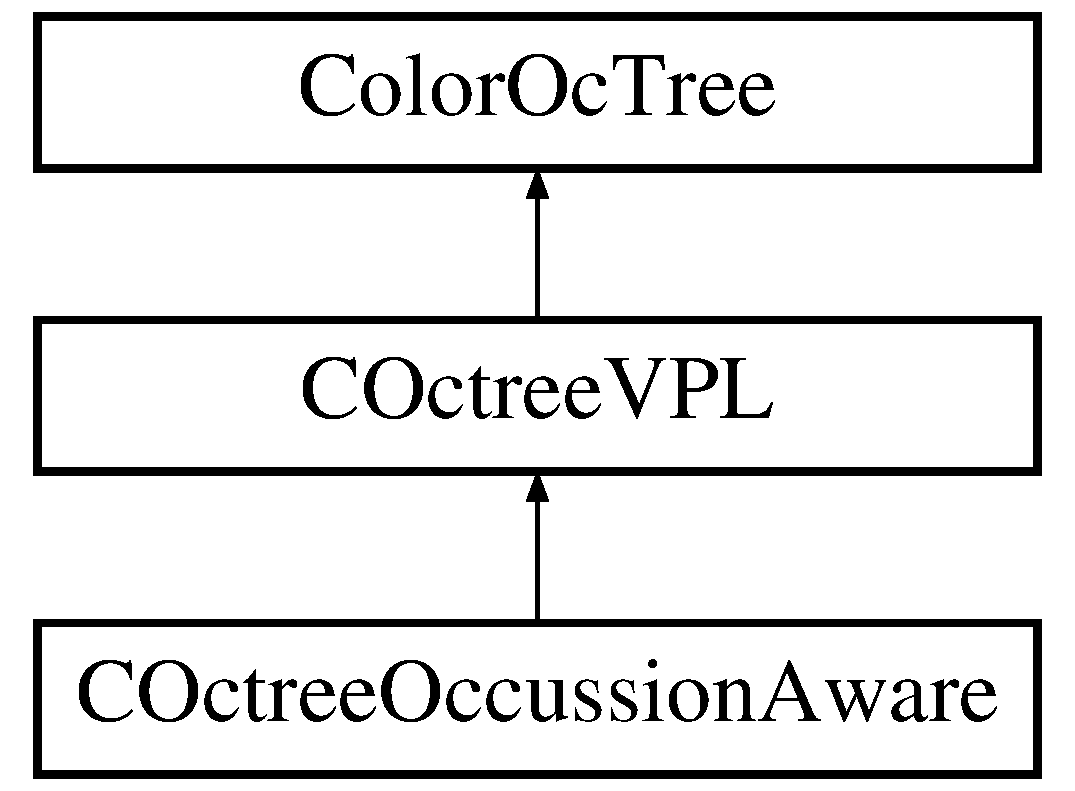
\includegraphics[height=3.000000cm]{classCOctreeOccussionAware}
\end{center}
\end{figure}
\subsection*{Additional Inherited Members}


The documentation for this class was generated from the following file\+:\begin{DoxyCompactItemize}
\item 
partialmodel/pmvoctreeoccusionaware.\+h\end{DoxyCompactItemize}

\hypertarget{classCOctreeRearSideVoxel}{}\section{C\+Octree\+Rear\+Side\+Voxel Class Reference}
\label{classCOctreeRearSideVoxel}\index{C\+Octree\+Rear\+Side\+Voxel@{C\+Octree\+Rear\+Side\+Voxel}}
Inheritance diagram for C\+Octree\+Rear\+Side\+Voxel\+:\begin{figure}[H]
\begin{center}
\leavevmode
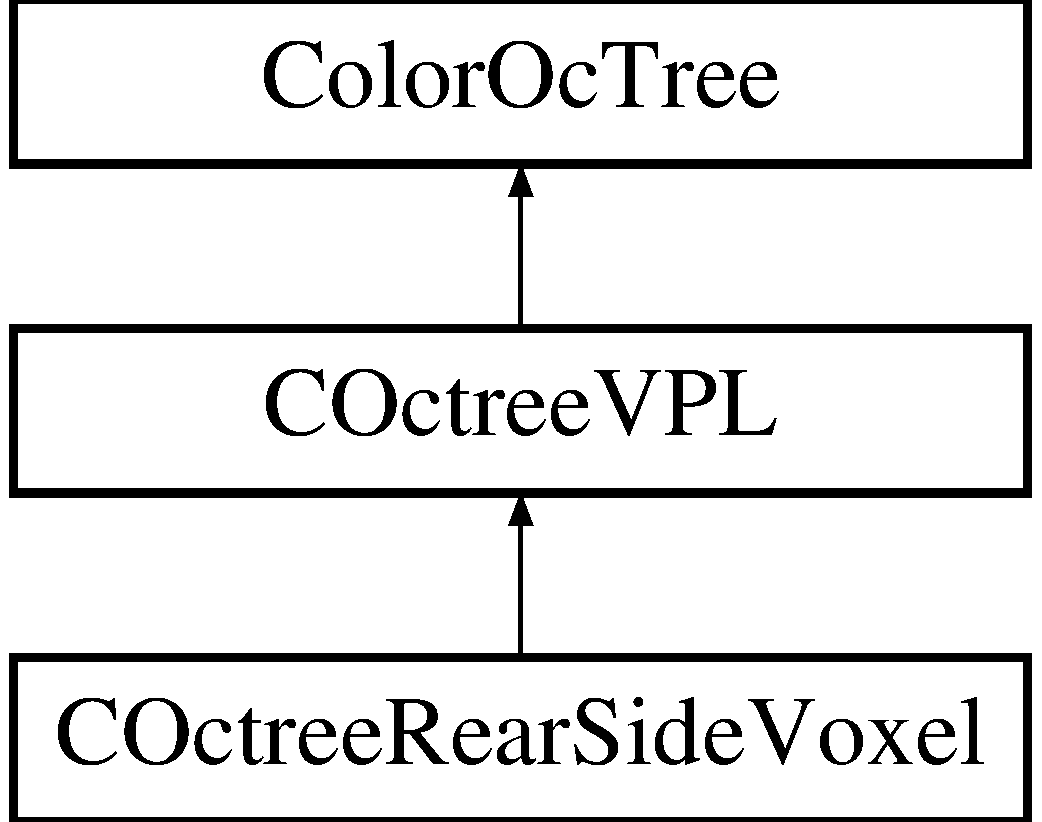
\includegraphics[height=3.000000cm]{classCOctreeRearSideVoxel}
\end{center}
\end{figure}
\subsection*{Public Member Functions}
\begin{DoxyCompactItemize}
\item 
{\bfseries C\+Octree\+Rear\+Side\+Voxel} (double resolution)\hypertarget{classCOctreeRearSideVoxel_a748a65035c7992eede6202ee632fdcc1}{}\label{classCOctreeRearSideVoxel_a748a65035c7992eede6202ee632fdcc1}

\end{DoxyCompactItemize}
\subsection*{Public Attributes}
\begin{DoxyCompactItemize}
\item 
octomap\+::\+Color\+Oc\+Tree\+Node\+::\+Color {\bfseries color\+Rear\+Side}\hypertarget{classCOctreeRearSideVoxel_a123be33074b8e80e0ee2305b6c543cbf}{}\label{classCOctreeRearSideVoxel_a123be33074b8e80e0ee2305b6c543cbf}

\end{DoxyCompactItemize}
\subsection*{Protected Member Functions}
\begin{DoxyCompactItemize}
\item 
virtual int \hyperlink{classCOctreeRearSideVoxel_a46ea49d079922e12ea62aff9ec8cae98}{cast\+Ray\+V\+PL} (const point3d \&origin, const point3d \&directionP, point3d \&end, bool ignore\+Unknown\+Cells=false, double max\+Range=-\/1.\+0)
\end{DoxyCompactItemize}
\subsection*{Additional Inherited Members}


\subsection{Member Function Documentation}
\index{C\+Octree\+Rear\+Side\+Voxel@{C\+Octree\+Rear\+Side\+Voxel}!cast\+Ray\+V\+PL@{cast\+Ray\+V\+PL}}
\index{cast\+Ray\+V\+PL@{cast\+Ray\+V\+PL}!C\+Octree\+Rear\+Side\+Voxel@{C\+Octree\+Rear\+Side\+Voxel}}
\subsubsection[{\texorpdfstring{cast\+Ray\+V\+P\+L(const point3d \&origin, const point3d \&direction\+P, point3d \&end, bool ignore\+Unknown\+Cells=false, double max\+Range=-\/1.\+0)}{castRayVPL(const point3d &origin, const point3d &directionP, point3d &end, bool ignoreUnknownCells=false, double maxRange=-1.0)}}]{\setlength{\rightskip}{0pt plus 5cm}int C\+Octree\+Rear\+Side\+Voxel\+::cast\+Ray\+V\+PL (
\begin{DoxyParamCaption}
\item[{const point3d \&}]{origin, }
\item[{const point3d \&}]{directionP, }
\item[{point3d \&}]{end, }
\item[{bool}]{ignore\+Unknown\+Cells = {\ttfamily false}, }
\item[{double}]{max\+Range = {\ttfamily -\/1.0}}
\end{DoxyParamCaption}
)\hspace{0.3cm}{\ttfamily [protected]}, {\ttfamily [virtual]}}\hypertarget{classCOctreeRearSideVoxel_a46ea49d079922e12ea62aff9ec8cae98}{}\label{classCOctreeRearSideVoxel_a46ea49d079922e12ea62aff9ec8cae98}
Traces a Ray in the octree and returns the type of voxel found It has been modified to return rearside voxels It does not return unknown voxels -\/-\/-\/-\/------ see Oc\+Tree\+Base\+::compute\+Ray\+Keys -\/-\/-\/-\/-\/------

cast\+Ray\+V\+PL !!!!! 

Reimplemented from \hyperlink{classCOctreeVPL_adefa863003c11fa51e87e9691bf860fa}{C\+Octree\+V\+PL}.



The documentation for this class was generated from the following files\+:\begin{DoxyCompactItemize}
\item 
partialmodel/pmvorearsidevoxel.\+h\item 
partialmodel/pmvorearsidevoxel.\+cpp\end{DoxyCompactItemize}

\hypertarget{classCOctreeVPL}{}\section{C\+Octree\+V\+PL Class Reference}
\label{classCOctreeVPL}\index{C\+Octree\+V\+PL@{C\+Octree\+V\+PL}}
Inheritance diagram for C\+Octree\+V\+PL\+:\begin{figure}[H]
\begin{center}
\leavevmode
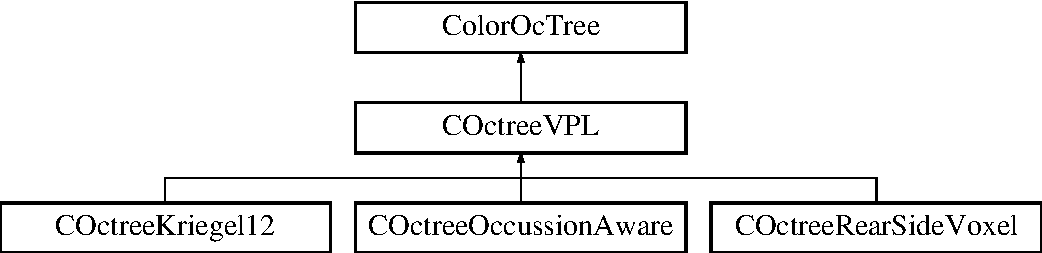
\includegraphics[height=3.000000cm]{classCOctreeVPL}
\end{center}
\end{figure}
\subsection*{Public Member Functions}
\begin{DoxyCompactItemize}
\item 
{\bfseries C\+Octree\+V\+PL} (double resolution)\hypertarget{classCOctreeVPL_a0149d4dd0aa97ad6c3bfe2ce5e52ae21}{}\label{classCOctreeVPL_a0149d4dd0aa97ad6c3bfe2ce5e52ae21}

\item 
virtual int \hyperlink{classCOctreeVPL_a8a57fc5e3499b794409ed83919260f99}{cast\+Ray\+V\+P\+L\+Hierarchical} (const point3d \&origin, const point3d \&directionP, point3d \&end, bool ignore\+Unknown\+Cells=false, double max\+Range=-\/1.\+0, int at\+Deepth=0)
\item 
virtual int \hyperlink{classCOctreeVPL_adefa863003c11fa51e87e9691bf860fa}{cast\+Ray\+V\+PL} (const point3d \&origin, const point3d \&directionP, point3d \&end, bool ignore\+Unknown\+Cells=false, double max\+Range=-\/1.\+0)
\item 
virtual double \hyperlink{classCOctreeVPL_a3a13d4e2bf90156a0bcc672feb2d521f}{cast\+Ray\+IG} (const point3d \&origin, const point3d \&directionP, point3d \&end, bool ignore\+Unknown\+Cells=false, double max\+Range=-\/1.\+0)
\item 
void \hyperlink{classCOctreeVPL_ac5612fe03561c785f3520b1c9f50177f}{clean\+Touched\+Voxels} ()
\item 
void {\bfseries set\+Unknown\+Thres} (double prob)\hypertarget{classCOctreeVPL_ab12c86b71ae63d2ce5ac9ecedb7bc852}{}\label{classCOctreeVPL_ab12c86b71ae63d2ce5ac9ecedb7bc852}

\item 
bool \hyperlink{classCOctreeVPL_aa708cc6dfe630232cbbf57401c90e37a}{is\+Node\+Unknown} (const Oc\+Tree\+Node $\ast$occupancy\+Node) const \hypertarget{classCOctreeVPL_aa708cc6dfe630232cbbf57401c90e37a}{}\label{classCOctreeVPL_aa708cc6dfe630232cbbf57401c90e37a}

\begin{DoxyCompactList}\small\item\em queries whether a node is occupied according to the tree\textquotesingle{}s parameter for \char`\"{}occupancy\char`\"{} \end{DoxyCompactList}\item 
bool \hyperlink{classCOctreeVPL_aac395e0f6092b287e4bf81c96b6f03ec}{is\+Node\+Unknown} (const Oc\+Tree\+Node \&occupancy\+Node) const \hypertarget{classCOctreeVPL_aac395e0f6092b287e4bf81c96b6f03ec}{}\label{classCOctreeVPL_aac395e0f6092b287e4bf81c96b6f03ec}

\begin{DoxyCompactList}\small\item\em queries whether a node is occupied according to the tree\textquotesingle{}s parameter for \char`\"{}occupancy\char`\"{} \end{DoxyCompactList}\item 
bool \hyperlink{classCOctreeVPL_a7860fba1bc74082821400b77042e665c}{is\+Node\+Free} (const Oc\+Tree\+Node $\ast$occupancy\+Node) const \hypertarget{classCOctreeVPL_a7860fba1bc74082821400b77042e665c}{}\label{classCOctreeVPL_a7860fba1bc74082821400b77042e665c}

\begin{DoxyCompactList}\small\item\em queries whether a node is occupied according to the tree\textquotesingle{}s parameter for \char`\"{}occupancy\char`\"{} \end{DoxyCompactList}\item 
bool {\bfseries is\+Adjacent\+To\+Free} (point3d point)\hypertarget{classCOctreeVPL_a7b15d06126f1033098558703d7b6aa61}{}\label{classCOctreeVPL_a7b15d06126f1033098558703d7b6aa61}

\item 
bool {\bfseries is\+Adjacent\+To\+Occupied} (point3d point)\hypertarget{classCOctreeVPL_abed99cc7f1dd56a9af7ab8a093e1115a}{}\label{classCOctreeVPL_abed99cc7f1dd56a9af7ab8a093e1115a}

\item 
void \hyperlink{classCOctreeVPL_aa4af367169533315e24760fd9ccbc0ea}{get\+Unknown\+Centers\+All} (point3d\+\_\+list \&node\+\_\+centers)
\item 
void \hyperlink{classCOctreeVPL_a0fbfbebbd0fb49f80159c4dc6f028401}{get\+Unknown\+Voxels} (point3d\+\_\+list \&node\+\_\+centers, std\+::vector$<$ double $>$ \&sizes)
\item 
void \hyperlink{classCOctreeVPL_abc10ca1c6e7119fe22430034bebf22f7}{get\+Visible\+Unknown\+Voxels} (point3d\+\_\+list \&node\+\_\+centers, point3d\+\_\+list \&voxel\+\_\+normals)
\item 
void \hyperlink{classCOctreeVPL_a08bd4856960a12a49078a451e20efb87}{get\+Frontier\+Unknown\+Voxels} (point3d\+\_\+list \&node\+\_\+centers, point3d\+\_\+list \&voxel\+\_\+normals)
\end{DoxyCompactItemize}
\subsection*{Public Attributes}
\begin{DoxyCompactItemize}
\item 
octomap\+::\+Color\+Oc\+Tree\+Node\+::\+Color {\bfseries color\+Touched\+Unknown}\hypertarget{classCOctreeVPL_a31d135d73813983ae78bf2b1763058ba}{}\label{classCOctreeVPL_a31d135d73813983ae78bf2b1763058ba}

\item 
octomap\+::\+Color\+Oc\+Tree\+Node\+::\+Color {\bfseries color\+Unknown}\hypertarget{classCOctreeVPL_afec2c69ea1c4c294a0b19d0d688cb95d}{}\label{classCOctreeVPL_afec2c69ea1c4c294a0b19d0d688cb95d}

\item 
octomap\+::\+Color\+Oc\+Tree\+Node\+::\+Color {\bfseries color\+Touched\+Occupied}\hypertarget{classCOctreeVPL_a9b80505c176da643abab260d36b0a8ca}{}\label{classCOctreeVPL_a9b80505c176da643abab260d36b0a8ca}

\item 
octomap\+::\+Color\+Oc\+Tree\+Node\+::\+Color {\bfseries color\+Occupied}\hypertarget{classCOctreeVPL_a9e4a135bf33774a080eee50a082c74ac}{}\label{classCOctreeVPL_a9e4a135bf33774a080eee50a082c74ac}

\end{DoxyCompactItemize}
\subsection*{Protected Attributes}
\begin{DoxyCompactItemize}
\item 
float {\bfseries unk\+\_\+prob\+\_\+thres\+\_\+log}\hypertarget{classCOctreeVPL_a1a2ec1493d8aa21c38210a0d7cb03956}{}\label{classCOctreeVPL_a1a2ec1493d8aa21c38210a0d7cb03956}

\item 
std\+::list$<$ Color\+Oc\+Tree\+Node $\ast$ $>$ {\bfseries touched\+Nodes}\hypertarget{classCOctreeVPL_ab4c73046dc8c049c8133fddffb93e09d}{}\label{classCOctreeVPL_ab4c73046dc8c049c8133fddffb93e09d}

\end{DoxyCompactItemize}


\subsection{Member Function Documentation}
\index{C\+Octree\+V\+PL@{C\+Octree\+V\+PL}!cast\+Ray\+IG@{cast\+Ray\+IG}}
\index{cast\+Ray\+IG@{cast\+Ray\+IG}!C\+Octree\+V\+PL@{C\+Octree\+V\+PL}}
\subsubsection[{\texorpdfstring{cast\+Ray\+I\+G(const point3d \&origin, const point3d \&direction\+P, point3d \&end, bool ignore\+Unknown\+Cells=false, double max\+Range=-\/1.\+0)}{castRayIG(const point3d &origin, const point3d &directionP, point3d &end, bool ignoreUnknownCells=false, double maxRange=-1.0)}}]{\setlength{\rightskip}{0pt plus 5cm}double C\+Octree\+V\+P\+L\+::cast\+Ray\+IG (
\begin{DoxyParamCaption}
\item[{const point3d \&}]{origin, }
\item[{const point3d \&}]{directionP, }
\item[{point3d \&}]{end, }
\item[{bool}]{ignore\+Unknown\+Cells = {\ttfamily false}, }
\item[{double}]{max\+Range = {\ttfamily -\/1.0}}
\end{DoxyParamCaption}
)\hspace{0.3cm}{\ttfamily [virtual]}}\hypertarget{classCOctreeVPL_a3a13d4e2bf90156a0bcc672feb2d521f}{}\label{classCOctreeVPL_a3a13d4e2bf90156a0bcc672feb2d521f}
Traces a Ray and returns the information gain of a ray. Avoids the integration of already touched voxels. Vasquez 17 and Vasquez 14. cast\+Ray Information Gain !!!!! 

Reimplemented in \hyperlink{classCOctreeKriegel12_aa900e135c79350675fb0b6a9ab5e3c02}{C\+Octree\+Kriegel12}.

\index{C\+Octree\+V\+PL@{C\+Octree\+V\+PL}!cast\+Ray\+V\+PL@{cast\+Ray\+V\+PL}}
\index{cast\+Ray\+V\+PL@{cast\+Ray\+V\+PL}!C\+Octree\+V\+PL@{C\+Octree\+V\+PL}}
\subsubsection[{\texorpdfstring{cast\+Ray\+V\+P\+L(const point3d \&origin, const point3d \&direction\+P, point3d \&end, bool ignore\+Unknown\+Cells=false, double max\+Range=-\/1.\+0)}{castRayVPL(const point3d &origin, const point3d &directionP, point3d &end, bool ignoreUnknownCells=false, double maxRange=-1.0)}}]{\setlength{\rightskip}{0pt plus 5cm}int C\+Octree\+V\+P\+L\+::cast\+Ray\+V\+PL (
\begin{DoxyParamCaption}
\item[{const point3d \&}]{origin, }
\item[{const point3d \&}]{directionP, }
\item[{point3d \&}]{end, }
\item[{bool}]{ignore\+Unknown\+Cells = {\ttfamily false}, }
\item[{double}]{max\+Range = {\ttfamily -\/1.0}}
\end{DoxyParamCaption}
)\hspace{0.3cm}{\ttfamily [virtual]}}\hypertarget{classCOctreeVPL_adefa863003c11fa51e87e9691bf860fa}{}\label{classCOctreeVPL_adefa863003c11fa51e87e9691bf860fa}
Traces a Ray in the octree and returns the type of voxel found -\/-\/-\/-\/------ see Oc\+Tree\+Base\+::compute\+Ray\+Keys -\/-\/-\/-\/-\/------

cast\+Ray\+V\+PL !!!!! 

Reimplemented in \hyperlink{classCOctreeRearSideVoxel_a46ea49d079922e12ea62aff9ec8cae98}{C\+Octree\+Rear\+Side\+Voxel}.

\index{C\+Octree\+V\+PL@{C\+Octree\+V\+PL}!cast\+Ray\+V\+P\+L\+Hierarchical@{cast\+Ray\+V\+P\+L\+Hierarchical}}
\index{cast\+Ray\+V\+P\+L\+Hierarchical@{cast\+Ray\+V\+P\+L\+Hierarchical}!C\+Octree\+V\+PL@{C\+Octree\+V\+PL}}
\subsubsection[{\texorpdfstring{cast\+Ray\+V\+P\+L\+Hierarchical(const point3d \&origin, const point3d \&direction\+P, point3d \&end, bool ignore\+Unknown\+Cells=false, double max\+Range=-\/1.\+0, int at\+Deepth=0)}{castRayVPLHierarchical(const point3d &origin, const point3d &directionP, point3d &end, bool ignoreUnknownCells=false, double maxRange=-1.0, int atDeepth=0)}}]{\setlength{\rightskip}{0pt plus 5cm}int C\+Octree\+V\+P\+L\+::cast\+Ray\+V\+P\+L\+Hierarchical (
\begin{DoxyParamCaption}
\item[{const point3d \&}]{origin, }
\item[{const point3d \&}]{directionP, }
\item[{point3d \&}]{end, }
\item[{bool}]{ignore\+Unknown\+Cells = {\ttfamily false}, }
\item[{double}]{max\+Range = {\ttfamily -\/1.0}, }
\item[{int}]{at\+Deepth = {\ttfamily 0}}
\end{DoxyParamCaption}
)\hspace{0.3cm}{\ttfamily [virtual]}}\hypertarget{classCOctreeVPL_a8a57fc5e3499b794409ed83919260f99}{}\label{classCOctreeVPL_a8a57fc5e3499b794409ed83919260f99}
Cast a ray for hierarchical ray tracing Traces a ray at a given octree depth This particular implementation paints the spanned voxels 
\begin{DoxyParams}{Parameters}
{\em end} & Return the last point \\
\hline
\end{DoxyParams}
Initialization phase -\/-\/-\/-\/-\/-\/-\/-\/-\/-\/-\/-\/-\/-\/-\/-\/-\/-\/-\/-\/-\/-\/-\/-\/-\/-\/-\/-\/-\/-\/-\/-\/-\/-\/-\/-\/-\/-\/-\/-\/-\/-\/-\/-\/-\/-\/-\/-\/-\/------

determinar la direccion \index{C\+Octree\+V\+PL@{C\+Octree\+V\+PL}!clean\+Touched\+Voxels@{clean\+Touched\+Voxels}}
\index{clean\+Touched\+Voxels@{clean\+Touched\+Voxels}!C\+Octree\+V\+PL@{C\+Octree\+V\+PL}}
\subsubsection[{\texorpdfstring{clean\+Touched\+Voxels()}{cleanTouchedVoxels()}}]{\setlength{\rightskip}{0pt plus 5cm}void C\+Octree\+V\+P\+L\+::clean\+Touched\+Voxels (
\begin{DoxyParamCaption}
{}
\end{DoxyParamCaption}
)}\hypertarget{classCOctreeVPL_ac5612fe03561c785f3520b1c9f50177f}{}\label{classCOctreeVPL_ac5612fe03561c785f3520b1c9f50177f}
This should be used after a ray tracing \index{C\+Octree\+V\+PL@{C\+Octree\+V\+PL}!get\+Frontier\+Unknown\+Voxels@{get\+Frontier\+Unknown\+Voxels}}
\index{get\+Frontier\+Unknown\+Voxels@{get\+Frontier\+Unknown\+Voxels}!C\+Octree\+V\+PL@{C\+Octree\+V\+PL}}
\subsubsection[{\texorpdfstring{get\+Frontier\+Unknown\+Voxels(point3d\+\_\+list \&node\+\_\+centers, point3d\+\_\+list \&voxel\+\_\+normals)}{getFrontierUnknownVoxels(point3d_list &node_centers, point3d_list &voxel_normals)}}]{\setlength{\rightskip}{0pt plus 5cm}void C\+Octree\+V\+P\+L\+::get\+Frontier\+Unknown\+Voxels (
\begin{DoxyParamCaption}
\item[{point3d\+\_\+list \&}]{node\+\_\+centers, }
\item[{point3d\+\_\+list \&}]{voxel\+\_\+normals}
\end{DoxyParamCaption}
)}\hypertarget{classCOctreeVPL_a08bd4856960a12a49078a451e20efb87}{}\label{classCOctreeVPL_a08bd4856960a12a49078a451e20efb87}
A frontier unknown voxel is a unknown voxel that is 6-\/adjacent to a free voxel and to a occupied voxel \index{C\+Octree\+V\+PL@{C\+Octree\+V\+PL}!get\+Unknown\+Centers\+All@{get\+Unknown\+Centers\+All}}
\index{get\+Unknown\+Centers\+All@{get\+Unknown\+Centers\+All}!C\+Octree\+V\+PL@{C\+Octree\+V\+PL}}
\subsubsection[{\texorpdfstring{get\+Unknown\+Centers\+All(point3d\+\_\+list \&node\+\_\+centers)}{getUnknownCentersAll(point3d_list &node_centers)}}]{\setlength{\rightskip}{0pt plus 5cm}void C\+Octree\+V\+P\+L\+::get\+Unknown\+Centers\+All (
\begin{DoxyParamCaption}
\item[{point3d\+\_\+list \&}]{node\+\_\+centers}
\end{DoxyParamCaption}
)}\hypertarget{classCOctreeVPL_aa4af367169533315e24760fd9ccbc0ea}{}\label{classCOctreeVPL_aa4af367169533315e24760fd9ccbc0ea}
Returns centers of all Uknown voxels, here all voxels that are inside the unknown probability range are used, plus leafs that do N\+OT exist (but could) in the set bounding box Upper and lower bounding points must be set before using this function \index{C\+Octree\+V\+PL@{C\+Octree\+V\+PL}!get\+Unknown\+Voxels@{get\+Unknown\+Voxels}}
\index{get\+Unknown\+Voxels@{get\+Unknown\+Voxels}!C\+Octree\+V\+PL@{C\+Octree\+V\+PL}}
\subsubsection[{\texorpdfstring{get\+Unknown\+Voxels(point3d\+\_\+list \&node\+\_\+centers, std\+::vector$<$ double $>$ \&sizes)}{getUnknownVoxels(point3d_list &node_centers, std::vector< double > &sizes)}}]{\setlength{\rightskip}{0pt plus 5cm}void C\+Octree\+V\+P\+L\+::get\+Unknown\+Voxels (
\begin{DoxyParamCaption}
\item[{point3d\+\_\+list \&}]{node\+\_\+centers, }
\item[{std\+::vector$<$ double $>$ \&}]{sizes}
\end{DoxyParamCaption}
)}\hypertarget{classCOctreeVPL_a0fbfbebbd0fb49f80159c4dc6f028401}{}\label{classCOctreeVPL_a0fbfbebbd0fb49f80159c4dc6f028401}
Returns centers of all Uknown voxels, here all voxels that are inside the unknown probability range are used, plus leafs that do N\+OT exist (but could) in the set bounding box Upper and lower bounding points must be set before using this function \index{C\+Octree\+V\+PL@{C\+Octree\+V\+PL}!get\+Visible\+Unknown\+Voxels@{get\+Visible\+Unknown\+Voxels}}
\index{get\+Visible\+Unknown\+Voxels@{get\+Visible\+Unknown\+Voxels}!C\+Octree\+V\+PL@{C\+Octree\+V\+PL}}
\subsubsection[{\texorpdfstring{get\+Visible\+Unknown\+Voxels(point3d\+\_\+list \&node\+\_\+centers, point3d\+\_\+list \&voxel\+\_\+normals)}{getVisibleUnknownVoxels(point3d_list &node_centers, point3d_list &voxel_normals)}}]{\setlength{\rightskip}{0pt plus 5cm}void C\+Octree\+V\+P\+L\+::get\+Visible\+Unknown\+Voxels (
\begin{DoxyParamCaption}
\item[{point3d\+\_\+list \&}]{node\+\_\+centers, }
\item[{point3d\+\_\+list \&}]{voxel\+\_\+normals}
\end{DoxyParamCaption}
)}\hypertarget{classCOctreeVPL_abc10ca1c6e7119fe22430034bebf22f7}{}\label{classCOctreeVPL_abc10ca1c6e7119fe22430034bebf22f7}
a visible unknown voxel is a unknown voxel that is 6-\/adjacent to a free voxel status\+: revised 

The documentation for this class was generated from the following files\+:\begin{DoxyCompactItemize}
\item 
partialmodel/coctreevpl.\+h\item 
partialmodel/coctreevpl.\+cpp\end{DoxyCompactItemize}

\hypertarget{classEvaluationResult}{}\section{Evaluation\+Result Class Reference}
\label{classEvaluationResult}\index{Evaluation\+Result@{Evaluation\+Result}}
\subsection*{Public Member Functions}
\begin{DoxyCompactItemize}
\item 
void {\bfseries clear} ()\hypertarget{classEvaluationResult_a5cb958df5f08e1c4d070f0ca6ae1514b}{}\label{classEvaluationResult_a5cb958df5f08e1c4d070f0ca6ae1514b}

\item 
void \hyperlink{classEvaluationResult_a529bd3f6b511988d0ddbbd2fee1e370b}{add\+Voxel\+Amouts} (\hyperlink{classEvaluationResult}{Evaluation\+Result} A)
\end{DoxyCompactItemize}
\subsection*{Public Attributes}
\begin{DoxyCompactItemize}
\item 
long int {\bfseries n\+\_\+occupied}\hypertarget{classEvaluationResult_af103614b995a13fc83595d64a8b199b9}{}\label{classEvaluationResult_af103614b995a13fc83595d64a8b199b9}

\item 
long int {\bfseries n\+\_\+unknown}\hypertarget{classEvaluationResult_ae43724b41f26e66dc2a5a6723d6509e2}{}\label{classEvaluationResult_ae43724b41f26e66dc2a5a6723d6509e2}

\item 
long int {\bfseries n\+\_\+occupied\+\_\+scene}\hypertarget{classEvaluationResult_a1cc45ff82e740750575694dc0e650adf}{}\label{classEvaluationResult_a1cc45ff82e740750575694dc0e650adf}

\item 
long int {\bfseries n\+\_\+unknown\+\_\+scene}\hypertarget{classEvaluationResult_afbd0c6e48cc3db5ddb7f1d8fd82a036d}{}\label{classEvaluationResult_afbd0c6e48cc3db5ddb7f1d8fd82a036d}

\item 
long int {\bfseries n\+\_\+lost}\hypertarget{classEvaluationResult_a4e5c5cee69789783cec8e7561cafde97}{}\label{classEvaluationResult_a4e5c5cee69789783cec8e7561cafde97}

\item 
long int {\bfseries n\+\_\+rear\+\_\+side}\hypertarget{classEvaluationResult_a778db5956b7a78f68ff2604d5d4c9313}{}\label{classEvaluationResult_a778db5956b7a78f68ff2604d5d4c9313}

\item 
float {\bfseries evaluation}\hypertarget{classEvaluationResult_aedb8f060d50873740bcce4069efd081f}{}\label{classEvaluationResult_aedb8f060d50873740bcce4069efd081f}

\item 
double {\bfseries computation\+\_\+time}\hypertarget{classEvaluationResult_aac898e8a214a5eb5dc76725c37fda7bb}{}\label{classEvaluationResult_aac898e8a214a5eb5dc76725c37fda7bb}

\end{DoxyCompactItemize}


\subsection{Member Function Documentation}
\index{Evaluation\+Result@{Evaluation\+Result}!add\+Voxel\+Amouts@{add\+Voxel\+Amouts}}
\index{add\+Voxel\+Amouts@{add\+Voxel\+Amouts}!Evaluation\+Result@{Evaluation\+Result}}
\subsubsection[{\texorpdfstring{add\+Voxel\+Amouts(\+Evaluation\+Result A)}{addVoxelAmouts(EvaluationResult A)}}]{\setlength{\rightskip}{0pt plus 5cm}void Evaluation\+Result\+::add\+Voxel\+Amouts (
\begin{DoxyParamCaption}
\item[{{\bf Evaluation\+Result}}]{A}
\end{DoxyParamCaption}
)}\hypertarget{classEvaluationResult_a529bd3f6b511988d0ddbbd2fee1e370b}{}\label{classEvaluationResult_a529bd3f6b511988d0ddbbd2fee1e370b}
Adds the voxel amouts

n\+\_\+lost += A.\+n\+\_\+lost; n\+\_\+occupied += A.\+n\+\_\+occupied; n\+\_\+occupied\+\_\+scene += A.\+n\+\_\+occupied\+\_\+scene; n\+\_\+unknown += A.\+n\+\_\+unknown; n\+\_\+unknown\+\_\+scene += A.\+n\+\_\+unknown\+\_\+scene; 

The documentation for this class was generated from the following files\+:\begin{DoxyCompactItemize}
\item 
partialmodel/evaluationresult.\+h\item 
partialmodel/evaluationresult.\+cpp\end{DoxyCompactItemize}

\hypertarget{classEvaluationResultVector}{}\section{Evaluation\+Result\+Vector Class Reference}
\label{classEvaluationResultVector}\index{Evaluation\+Result\+Vector@{Evaluation\+Result\+Vector}}
Inheritance diagram for Evaluation\+Result\+Vector\+:\begin{figure}[H]
\begin{center}
\leavevmode
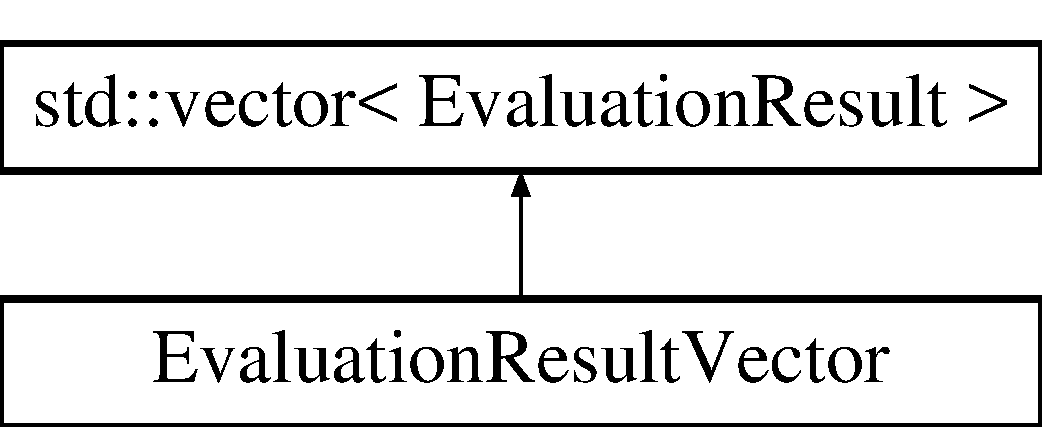
\includegraphics[height=2.000000cm]{classEvaluationResultVector}
\end{center}
\end{figure}
\subsection*{Public Member Functions}
\begin{DoxyCompactItemize}
\item 
void {\bfseries save\+Vector} (std\+::string file\+\_\+name)\hypertarget{classEvaluationResultVector_a5f4b52d9b54b911a77505b168fe16aba}{}\label{classEvaluationResultVector_a5f4b52d9b54b911a77505b168fe16aba}

\end{DoxyCompactItemize}


The documentation for this class was generated from the following files\+:\begin{DoxyCompactItemize}
\item 
partialmodel/evaluationresult.\+h\item 
partialmodel/evaluationresult.\+cpp\end{DoxyCompactItemize}

\hypertarget{classINIReader}{}\section{I\+N\+I\+Reader Class Reference}
\label{classINIReader}\index{I\+N\+I\+Reader@{I\+N\+I\+Reader}}
\subsection*{Public Member Functions}
\begin{DoxyCompactItemize}
\item 
{\bfseries I\+N\+I\+Reader} (std\+::string filename)\hypertarget{classINIReader_a357e21f6b1bc10b17bd3a7b72452cb57}{}\label{classINIReader_a357e21f6b1bc10b17bd3a7b72452cb57}

\item 
int {\bfseries Parse\+Error} ()\hypertarget{classINIReader_aaecb5fce7bfeac1710b3a7d5f7ec94ab}{}\label{classINIReader_aaecb5fce7bfeac1710b3a7d5f7ec94ab}

\item 
std\+::set$<$ std\+::string $>$ {\bfseries Sections} ()\hypertarget{classINIReader_a8dc6b10ba3415f3c30c30c4fc342d867}{}\label{classINIReader_a8dc6b10ba3415f3c30c30c4fc342d867}

\item 
std\+::string {\bfseries Get} (std\+::string section, std\+::string name, std\+::string default\+\_\+value)\hypertarget{classINIReader_a1042bfbb483afa305283a6f1a2bf27e9}{}\label{classINIReader_a1042bfbb483afa305283a6f1a2bf27e9}

\item 
long {\bfseries Get\+Integer} (std\+::string section, std\+::string name, long default\+\_\+value)\hypertarget{classINIReader_a5fb288f961b8a43ba4974fbf97f4d1df}{}\label{classINIReader_a5fb288f961b8a43ba4974fbf97f4d1df}

\item 
double {\bfseries Get\+Real} (std\+::string section, std\+::string name, double default\+\_\+value)\hypertarget{classINIReader_add45ae10b48fd12cb98a7b73e67d3a77}{}\label{classINIReader_add45ae10b48fd12cb98a7b73e67d3a77}

\item 
bool {\bfseries Get\+Boolean} (std\+::string section, std\+::string name, bool default\+\_\+value)\hypertarget{classINIReader_ac3d70858d357a6797b0d58a9a00d737e}{}\label{classINIReader_ac3d70858d357a6797b0d58a9a00d737e}

\end{DoxyCompactItemize}


The documentation for this class was generated from the following file\+:\begin{DoxyCompactItemize}
\item 
partialmodel/I\+N\+I\+Reader.\+h\end{DoxyCompactItemize}

\hypertarget{classNBVPlanner}{}\section{N\+B\+V\+Planner Class Reference}
\label{classNBVPlanner}\index{N\+B\+V\+Planner@{N\+B\+V\+Planner}}


{\ttfamily \#include $<$nbvplanner.\+h$>$}

Inheritance diagram for N\+B\+V\+Planner\+:\begin{figure}[H]
\begin{center}
\leavevmode
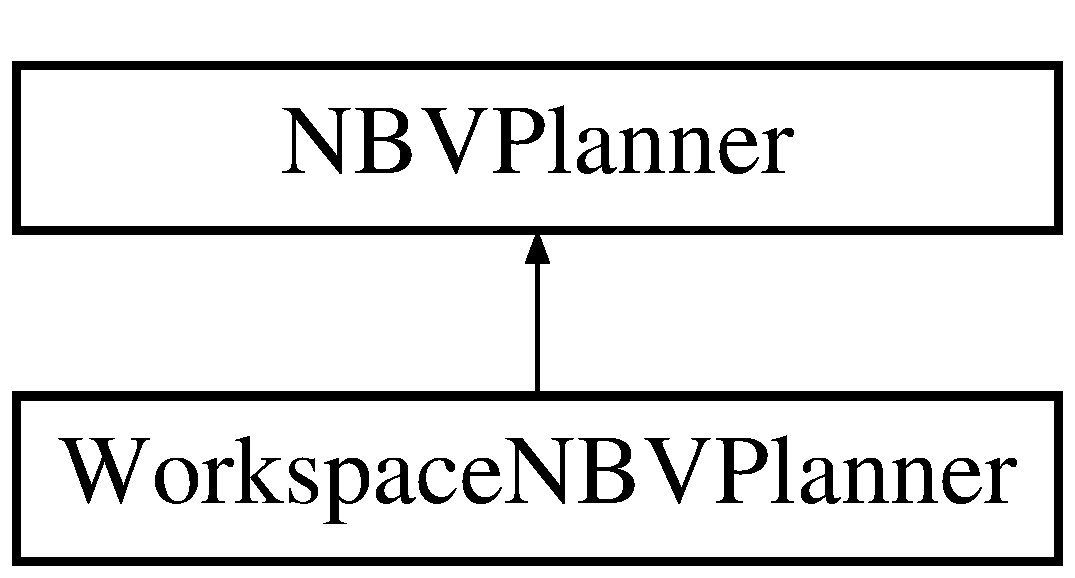
\includegraphics[height=3.000000cm]{classNBVPlanner}
\end{center}
\end{figure}
\subsection*{Public Member Functions}
\begin{DoxyCompactItemize}
\item 
{\bfseries N\+B\+V\+Planner} (\hyperlink{classRobotSensor}{Robot\+Sensor} $\ast$rs, \hyperlink{classPartialModelBase}{Partial\+Model\+Base} $\ast$pm)\hypertarget{classNBVPlanner_afeaf82f7d6ee61346e796e26cd4730bb}{}\label{classNBVPlanner_afeaf82f7d6ee61346e796e26cd4730bb}

\item 
virtual bool {\bfseries init} ()\hypertarget{classNBVPlanner_aee188426e3324afa0875c7b030370d73}{}\label{classNBVPlanner_aee188426e3324afa0875c7b030370d73}

\item 
void {\bfseries get\+Solution\+Controls} (std\+::vector$<$ std\+::vector$<$ double $>$ $>$ \&controls, double \&delta\+\_\+t)\hypertarget{classNBVPlanner_a674fb1af1257cd3ce5aa0508f5c53ff0}{}\label{classNBVPlanner_a674fb1af1257cd3ce5aa0508f5c53ff0}

\item 
void {\bfseries get\+Solution\+Path} (std\+::vector$<$ std\+::vector$<$ double $>$ $>$ \&path)\hypertarget{classNBVPlanner_a68515cd88fcadd94e51c625be381ff75}{}\label{classNBVPlanner_a68515cd88fcadd94e51c625be381ff75}

\item 
void {\bfseries set\+Config\+Folder} (std\+::string folder)\hypertarget{classNBVPlanner_a8c8809f55beee71c693c3da15fc92b33}{}\label{classNBVPlanner_a8c8809f55beee71c693c3da15fc92b33}

\item 
void {\bfseries set\+Data\+Folder} (std\+::string folder)\hypertarget{classNBVPlanner_abaf6c50fd3e63cdab95703d73aeb13fe}{}\label{classNBVPlanner_abaf6c50fd3e63cdab95703d73aeb13fe}

\item 
virtual float \hyperlink{classNBVPlanner_a97e09f3acac040f3bd1bfc990fc1fce4}{update\+With\+Poin\+Cloud} (std\+::string pc\+\_\+file, std\+::string origin\+\_\+file)
\item 
virtual bool \hyperlink{classNBVPlanner_a448567c9d5cec319c5df5efdb0d5479c}{plan\+N\+BV} (\hyperlink{classViewStructure}{View\+Structure} \&v)=0
\item 
virtual bool {\bfseries save\+Partial\+Model} (std\+::string file\+\_\+name)\hypertarget{classNBVPlanner_a452136c3c1637976cbf2996d6006e27a}{}\label{classNBVPlanner_a452136c3c1637976cbf2996d6006e27a}

\item 
void {\bfseries finish\+Planning} ()\hypertarget{classNBVPlanner_a4cf0672ba39ae9dc42e64230d744a4bd}{}\label{classNBVPlanner_a4cf0672ba39ae9dc42e64230d744a4bd}

\item 
bool \hyperlink{classNBVPlanner_abf09392a8294aa537c7adda5f302d2e7}{save\+Planner\+Data} ()
\end{DoxyCompactItemize}
\subsection*{Public Attributes}
\begin{DoxyCompactItemize}
\item 
float \hyperlink{classNBVPlanner_afa873ac12ea806f933b96d2ffc71b49e}{std\+\_\+v\+\_\+time}\hypertarget{classNBVPlanner_afa873ac12ea806f933b96d2ffc71b49e}{}\label{classNBVPlanner_afa873ac12ea806f933b96d2ffc71b49e}

\begin{DoxyCompactList}\small\item\em statistical variables \end{DoxyCompactList}\item 
float {\bfseries std\+\_\+mp\+\_\+time}\hypertarget{classNBVPlanner_ae785f31f58caa631c1cbce54598d427a}{}\label{classNBVPlanner_ae785f31f58caa631c1cbce54598d427a}

\item 
float {\bfseries std\+\_\+distance}\hypertarget{classNBVPlanner_a2e71279cedd2afb6553ac253308e1a6b}{}\label{classNBVPlanner_a2e71279cedd2afb6553ac253308e1a6b}

\item 
float {\bfseries std\+\_\+accu\+\_\+distance}\hypertarget{classNBVPlanner_af3eb12dbbf9c649bb8d8795640b9f358}{}\label{classNBVPlanner_af3eb12dbbf9c649bb8d8795640b9f358}

\item 
float {\bfseries std\+\_\+utility}\hypertarget{classNBVPlanner_a3d310ebb2eb5b172be1313d89f011b7c}{}\label{classNBVPlanner_a3d310ebb2eb5b172be1313d89f011b7c}

\item 
float {\bfseries std\+\_\+surface\+\_\+uf}\hypertarget{classNBVPlanner_a4741a474d0f13a079dc4e65263dba746}{}\label{classNBVPlanner_a4741a474d0f13a079dc4e65263dba746}

\item 
float {\bfseries std\+\_\+distance\+\_\+uf}\hypertarget{classNBVPlanner_a523a5928df4a3cdd7dc0f408d6712c2b}{}\label{classNBVPlanner_a523a5928df4a3cdd7dc0f408d6712c2b}

\end{DoxyCompactItemize}
\subsection*{Protected Attributes}
\begin{DoxyCompactItemize}
\item 
\hyperlink{classRobotSensor}{Robot\+Sensor} $\ast$ {\bfseries robot\+With\+Sensor}\hypertarget{classNBVPlanner_a6fec8a79d56dc35f51905ce2abeff0c6}{}\label{classNBVPlanner_a6fec8a79d56dc35f51905ce2abeff0c6}

\item 
\hyperlink{classPartialModelBase}{Partial\+Model\+Base} $\ast$ {\bfseries partial\+Model}\hypertarget{classNBVPlanner_a4e0ce42f393fed4546eee0249c71c7d4}{}\label{classNBVPlanner_a4e0ce42f393fed4546eee0249c71c7d4}

\item 
\hyperlink{classViewStructure}{View\+Structure} {\bfseries N\+BV}\hypertarget{classNBVPlanner_ac985d89444c084511403e5f5378dc125}{}\label{classNBVPlanner_ac985d89444c084511403e5f5378dc125}

\item 
std\+::vector$<$ std\+::vector$<$ double $>$ $>$ {\bfseries solution\+Controls}\hypertarget{classNBVPlanner_acebd542969897418dbdd03bd41e38dac}{}\label{classNBVPlanner_acebd542969897418dbdd03bd41e38dac}

\item 
std\+::vector$<$ std\+::vector$<$ double $>$ $>$ {\bfseries solution\+Path}\hypertarget{classNBVPlanner_acdc8f98e9d26646edec5c23fe391e980}{}\label{classNBVPlanner_acdc8f98e9d26646edec5c23fe391e980}

\item 
double {\bfseries planner\+DeltaT}\hypertarget{classNBVPlanner_a1ad75582b63a705ef2014ef6e6f550a2}{}\label{classNBVPlanner_a1ad75582b63a705ef2014ef6e6f550a2}

\item 
long int {\bfseries rrt\+Nodes}\hypertarget{classNBVPlanner_a824b421ac2e61a6f4636890198007f76}{}\label{classNBVPlanner_a824b421ac2e61a6f4636890198007f76}

\item 
std\+::string {\bfseries config\+Folder}\hypertarget{classNBVPlanner_a0d891b635bf4857e4a8cf6553d492b4b}{}\label{classNBVPlanner_a0d891b635bf4857e4a8cf6553d492b4b}

\item 
std\+::string {\bfseries data\+Folder}\hypertarget{classNBVPlanner_a12861032ba435a8bf036eaa9ca59584a}{}\label{classNBVPlanner_a12861032ba435a8bf036eaa9ca59584a}

\item 
std\+::vector$<$ float $>$ \hyperlink{classNBVPlanner_a00c0db5c287885f94ef0c21d79a4df4a}{vision\+Times}\hypertarget{classNBVPlanner_a00c0db5c287885f94ef0c21d79a4df4a}{}\label{classNBVPlanner_a00c0db5c287885f94ef0c21d79a4df4a}

\begin{DoxyCompactList}\small\item\em statistical variables \end{DoxyCompactList}\item 
std\+::vector$<$ float $>$ {\bfseries motion\+P\+Times}\hypertarget{classNBVPlanner_aa4bca56e281856c30e4b251d5dd69235}{}\label{classNBVPlanner_aa4bca56e281856c30e4b251d5dd69235}

\item 
std\+::vector$<$ double $>$ {\bfseries distances\+\_\+per\+\_\+it}\hypertarget{classNBVPlanner_aca3c5b4b9beabea33f8a58e5306aa5ee}{}\label{classNBVPlanner_aca3c5b4b9beabea33f8a58e5306aa5ee}

\end{DoxyCompactItemize}


\subsection{Detailed Description}
Planner base class 

\subsection{Member Function Documentation}
\index{N\+B\+V\+Planner@{N\+B\+V\+Planner}!plan\+N\+BV@{plan\+N\+BV}}
\index{plan\+N\+BV@{plan\+N\+BV}!N\+B\+V\+Planner@{N\+B\+V\+Planner}}
\subsubsection[{\texorpdfstring{plan\+N\+B\+V(\+View\+Structure \&v)=0}{planNBV(ViewStructure &v)=0}}]{\setlength{\rightskip}{0pt plus 5cm}virtual bool N\+B\+V\+Planner\+::plan\+N\+BV (
\begin{DoxyParamCaption}
\item[{{\bf View\+Structure} \&}]{v}
\end{DoxyParamCaption}
)\hspace{0.3cm}{\ttfamily [pure virtual]}}\hypertarget{classNBVPlanner_a448567c9d5cec319c5df5efdb0d5479c}{}\label{classNBVPlanner_a448567c9d5cec319c5df5efdb0d5479c}
Main function, it computes the N\+BV 

Implemented in \hyperlink{classWorkspaceNBVPlanner_ad5655e5c1c45a017d4c598fd2632ed49}{Workspace\+N\+B\+V\+Planner}, and \hyperlink{classTrainingPlanner_a9c82d194af01b8edf4d34a34e36c4c8c}{Training\+Planner}.

\index{N\+B\+V\+Planner@{N\+B\+V\+Planner}!save\+Planner\+Data@{save\+Planner\+Data}}
\index{save\+Planner\+Data@{save\+Planner\+Data}!N\+B\+V\+Planner@{N\+B\+V\+Planner}}
\subsubsection[{\texorpdfstring{save\+Planner\+Data()}{savePlannerData()}}]{\setlength{\rightskip}{0pt plus 5cm}bool N\+B\+V\+Planner\+::save\+Planner\+Data (
\begin{DoxyParamCaption}
{}
\end{DoxyParamCaption}
)}\hypertarget{classNBVPlanner_abf09392a8294aa537c7adda5f302d2e7}{}\label{classNBVPlanner_abf09392a8294aa537c7adda5f302d2e7}
Guardar datos del R\+R\+T\+N\+BV

Save Obstacle information \index{N\+B\+V\+Planner@{N\+B\+V\+Planner}!update\+With\+Poin\+Cloud@{update\+With\+Poin\+Cloud}}
\index{update\+With\+Poin\+Cloud@{update\+With\+Poin\+Cloud}!N\+B\+V\+Planner@{N\+B\+V\+Planner}}
\subsubsection[{\texorpdfstring{update\+With\+Poin\+Cloud(std\+::string pc\+\_\+file, std\+::string origin\+\_\+file)}{updateWithPoinCloud(std::string pc_file, std::string origin_file)}}]{\setlength{\rightskip}{0pt plus 5cm}float N\+B\+V\+Planner\+::update\+With\+Poin\+Cloud (
\begin{DoxyParamCaption}
\item[{std\+::string}]{pc\+\_\+file, }
\item[{std\+::string}]{origin\+\_\+file}
\end{DoxyParamCaption}
)\hspace{0.3cm}{\ttfamily [virtual]}}\hypertarget{classNBVPlanner_a97e09f3acac040f3bd1bfc990fc1fce4}{}\label{classNBVPlanner_a97e09f3acac040f3bd1bfc990fc1fce4}
The planner updates its internal representation for example octree 

The documentation for this class was generated from the following files\+:\begin{DoxyCompactItemize}
\item 
viewplanning/nbvplanner.\+h\item 
viewplanning/nbvplanner.\+cpp\end{DoxyCompactItemize}

\hypertarget{classPartialModelBase}{}\section{Partial\+Model\+Base Class Reference}
\label{classPartialModelBase}\index{Partial\+Model\+Base@{Partial\+Model\+Base}}


{\ttfamily \#include $<$partialmodelbase.\+h$>$}

Inheritance diagram for Partial\+Model\+Base\+:\begin{figure}[H]
\begin{center}
\leavevmode
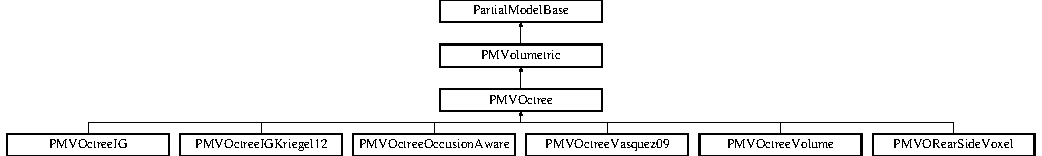
\includegraphics[height=2.097378cm]{classPartialModelBase}
\end{center}
\end{figure}
\subsection*{Public Member Functions}
\begin{DoxyCompactItemize}
\item 
virtual float {\bfseries update\+With\+Scan} (std\+::string file\+\_\+name\+\_\+scan, std\+::string file\+\_\+name\+\_\+origin)=0\hypertarget{classPartialModelBase_a7071062d9a064fbc4bc62451db9390e3}{}\label{classPartialModelBase_a7071062d9a064fbc4bc62451db9390e3}

\item 
virtual void {\bfseries evaluate\+Candidate\+Views} ()\hypertarget{classPartialModelBase_ad7bc3e7e78b330b960de7ea36bc0dbff}{}\label{classPartialModelBase_ad7bc3e7e78b330b960de7ea36bc0dbff}

\item 
void {\bfseries evaluate\+Candidate\+Views} (\hyperlink{classViewList}{View\+List} \&views)\hypertarget{classPartialModelBase_a84680a7a9806e6816c29585a39109696}{}\label{classPartialModelBase_a84680a7a9806e6816c29585a39109696}

\item 
virtual int {\bfseries evaluate\+View} (\hyperlink{classViewStructure}{View\+Structure} \&v)=0\hypertarget{classPartialModelBase_a4f5c7099d776cefb4c67fc89613e5cac}{}\label{classPartialModelBase_a4f5c7099d776cefb4c67fc89613e5cac}

\item 
virtual bool {\bfseries stop\+Criteria\+Reached} ()=0\hypertarget{classPartialModelBase_aee7942b3450482f70d2b281ab26c6336}{}\label{classPartialModelBase_aee7942b3450482f70d2b281ab26c6336}

\item 
virtual bool {\bfseries save\+Partial\+Model} (std\+::string file\+\_\+name)=0\hypertarget{classPartialModelBase_a1586ba365b880e7e3241fba1168b58cd}{}\label{classPartialModelBase_a1586ba365b880e7e3241fba1168b58cd}

\item 
virtual bool {\bfseries load\+Partial\+Model} (std\+::string file\+\_\+name)=0\hypertarget{classPartialModelBase_a543970b4e4066f26be64b41f3c4738be}{}\label{classPartialModelBase_a543970b4e4066f26be64b41f3c4738be}

\item 
virtual double \hyperlink{classPartialModelBase_a3dc1ffa43084246c6a79b5763025dc73}{get\+Unknown\+Volume} ()=0
\item 
virtual long int \hyperlink{classPartialModelBase_a645f1e68e3e29419522c3ef10ee05d05}{read\+Rays} (std\+::string file\+\_\+address)=0
\item 
virtual bool {\bfseries init} ()\hypertarget{classPartialModelBase_a6c031ab6c30539668c840d440d5a5513}{}\label{classPartialModelBase_a6c031ab6c30539668c840d440d5a5513}

\item 
bool \hyperlink{classPartialModelBase_a270503fb56c16b85f36c71f633513452}{save\+Evaluated\+Views} (std\+::string file\+\_\+name)
\item 
bool \hyperlink{classPartialModelBase_a3552efe44c5a12299c7462e35d9fd75e}{read\+Candidate\+Views} (std\+::string file\+\_\+name)
\item 
bool \hyperlink{classPartialModelBase_aa76eab3ce386966f7f65069c44f8f895}{save\+Only\+N\+Views} (int n, std\+::string file\+\_\+name)
\item 
void \hyperlink{classPartialModelBase_a745fab1e7b26b3a8f1efed66d69ef41a}{sort\+Candidate\+Views} ()
\item 
void \hyperlink{classPartialModelBase_a7dee7d3e7bb81092fa7f74709fb4996f}{set\+Object\+Capsule} (double x1, double y1, double z1, double x2, double y2, double z2)
\item 
void \hyperlink{classPartialModelBase_ac848bd32ebc54d49c9a8adb0d25e31ec}{set\+Scene} (double x1, double y1, double z1, double x2, double y2, double z2)
\item 
void {\bfseries set\+Config\+Folder} (std\+::string folder)\hypertarget{classPartialModelBase_a2b43f5a70a4c3ca94ee5c8939717b6ac}{}\label{classPartialModelBase_a2b43f5a70a4c3ca94ee5c8939717b6ac}

\item 
void {\bfseries set\+Data\+Folder} (std\+::string folder)\hypertarget{classPartialModelBase_a5a19a9366db46a1dfa95c8b2a9e1e8d3}{}\label{classPartialModelBase_a5a19a9366db46a1dfa95c8b2a9e1e8d3}

\item 
virtual void {\bfseries save\+Evaluations} ()=0\hypertarget{classPartialModelBase_a9cdef7a86e8c039520937eee049686a0}{}\label{classPartialModelBase_a9cdef7a86e8c039520937eee049686a0}

\item 
virtual void \hyperlink{classPartialModelBase_a193634a1ffbc43b60164dae988204d9e}{save\+Object\+As\+RawT} (std\+::string file\+\_\+name)=0
\item 
virtual void \hyperlink{classPartialModelBase_a994da889db902ef5948d9db48609d00b}{save\+Object\+As\+Obst} (std\+::string file\+\_\+name)=0
\item 
virtual bool \hyperlink{classPartialModelBase_a6b5f29ca5354d246ec08af21f764552e}{save\+Unknown\+Volume\+As\+Obst} (std\+::string file\+\_\+name)=0
\item 
virtual bool \hyperlink{classPartialModelBase_a2f0c03925d1afc098dede157d0876ee3}{save\+Unknown\+Volume\+As\+RawT} (std\+::string file\+\_\+name)=0
\item 
virtual bool \hyperlink{classPartialModelBase_ab41193a2a697dcf0d7d416cb35836458}{save\+Obstacle} (std\+::string file\+\_\+name)=0
\item 
virtual bool {\bfseries save\+Visible\+Unknown} (std\+::string file\+\_\+name\+\_\+vertex, std\+::string file\+\_\+name\+\_\+normal)=0\hypertarget{classPartialModelBase_a5304bbb21ba2a3bda34c300cfa628d36}{}\label{classPartialModelBase_a5304bbb21ba2a3bda34c300cfa628d36}

\item 
virtual bool {\bfseries save\+Frontier\+Unknown} (std\+::string file\+\_\+name\+\_\+vertex, std\+::string file\+\_\+name\+\_\+normal)=0\hypertarget{classPartialModelBase_a5f71113c57da42c730929af0eb6d59ba}{}\label{classPartialModelBase_a5f71113c57da42c730929af0eb6d59ba}

\item 
virtual void {\bfseries get\+Occupied\+Triangles} (\hyperlink{classvpTriangleList}{vp\+Triangle\+List} \&tris)=0\hypertarget{classPartialModelBase_af66511a5e5679937fd4b393fb11a49ed}{}\label{classPartialModelBase_af66511a5e5679937fd4b393fb11a49ed}

\item 
virtual void {\bfseries get\+Unknown\+Triangles} (\hyperlink{classvpTriangleList}{vp\+Triangle\+List} \&tris)=0\hypertarget{classPartialModelBase_a4dc17a79b5713384c08561bc74b416c0}{}\label{classPartialModelBase_a4dc17a79b5713384c08561bc74b416c0}

\item 
void \hyperlink{classPartialModelBase_a60fa44bbde343902f8adfce270b27b87}{get\+O\+BB} (double \&x1, double \&y1, double \&z1, double \&x2, double \&y2, double \&z2)
\item 
bool {\bfseries poits\+To\+The\+Object} (\hyperlink{classViewStructure}{View\+Structure} \&v)\hypertarget{classPartialModelBase_af0c4f683c0d35469b366d91c5851022a}{}\label{classPartialModelBase_af0c4f683c0d35469b366d91c5851022a}

\end{DoxyCompactItemize}
\subsection*{Public Attributes}
\begin{DoxyCompactItemize}
\item 
std\+::string \hyperlink{classPartialModelBase_a7baf1e6dfaaf4891b6ac03cbafc7e4d2}{object\+\_\+points\+\_\+filename}
\end{DoxyCompactItemize}
\subsection*{Protected Member Functions}
\begin{DoxyCompactItemize}
\item 
bool {\bfseries points\+To\+A\+Sphere} (\hyperlink{classViewStructure}{View\+Structure} \&v, double center\+\_\+x, double center\+\_\+y, double center\+\_\+z, double radius)\hypertarget{classPartialModelBase_a926130c2455fb010d50bccc0850494a6}{}\label{classPartialModelBase_a926130c2455fb010d50bccc0850494a6}

\item 
bool \hyperlink{classPartialModelBase_a6f91d65d4a984f3b1ccdd1ac5abfd070}{is\+In\+D\+OV} (octomap\+::point3d origin, octomap\+::point3d point)
\item 
bool \hyperlink{classPartialModelBase_a7336ed5fc1bf4d2e0849d35e0e1070c5}{is\+In\+Capsule} (octomap\+::point3d point)
\item 
bool {\bfseries is\+In\+Scene} (octomap\+::point3d point)\hypertarget{classPartialModelBase_a1b8dc9293182a3524ba9288c949b4943}{}\label{classPartialModelBase_a1b8dc9293182a3524ba9288c949b4943}

\item 
virtual bool \hyperlink{classPartialModelBase_a3e8464488605e9f5ef17a3e641b29429}{registration\+Low\+Constraint} (long int n\+\_\+occupied)
\item 
bool \hyperlink{classPartialModelBase_a7516301463e716f3d5f086315844ca86}{read\+Point\+Cloud\+From\+D\+AT} (std\+::string file\+\_\+name, octomap\+::\+Pointcloud \&cloud)
\item 
void {\bfseries compute\+Ray\+From\+Origin\+To\+Point} (double x, double y, double z, double \&i, double \&j, double \&k)\hypertarget{classPartialModelBase_ad5563edf4a7860474e3a8420f60d4379}{}\label{classPartialModelBase_ad5563edf4a7860474e3a8420f60d4379}

\item 
void {\bfseries compute\+Ray\+From\+Point\+To\+Point} (Boost\+Matrix pointA, Boost\+Matrix pointB, double \&i, double \&j, double \&k)\hypertarget{classPartialModelBase_a922dac8a6cf6799d41d4dabc79695664}{}\label{classPartialModelBase_a922dac8a6cf6799d41d4dabc79695664}

\end{DoxyCompactItemize}
\subsection*{Protected Attributes}
\begin{DoxyCompactItemize}
\item 
Pointcloud \hyperlink{classPartialModelBase_aea17bd2912ce2a10534aebc7b9cb1bd0}{object\+Point\+Cloud}\hypertarget{classPartialModelBase_aea17bd2912ce2a10534aebc7b9cb1bd0}{}\label{classPartialModelBase_aea17bd2912ce2a10534aebc7b9cb1bd0}

\begin{DoxyCompactList}\small\item\em Object accumulated point cloud. \end{DoxyCompactList}\item 
point3d {\bfseries object\+Sphere\+Center}\hypertarget{classPartialModelBase_ad10f278864d170acb63b67554b6fda85}{}\label{classPartialModelBase_ad10f278864d170acb63b67554b6fda85}

\item 
double {\bfseries object\+Sphere\+Radius}\hypertarget{classPartialModelBase_a934a90b49dc60e614af6c13d2d9a9f49}{}\label{classPartialModelBase_a934a90b49dc60e614af6c13d2d9a9f49}

\item 
double {\bfseries obj\+Radius2}\hypertarget{classPartialModelBase_ad14118b3b5ec4db4566e3cb9d3f04224}{}\label{classPartialModelBase_ad14118b3b5ec4db4566e3cb9d3f04224}

\item 
point3d {\bfseries director\+Ray}\hypertarget{classPartialModelBase_add9d606ad4e0594a735a7518723a9bf7}{}\label{classPartialModelBase_add9d606ad4e0594a735a7518723a9bf7}

\item 
std\+::string {\bfseries config\+Folder}\hypertarget{classPartialModelBase_abfdf8b46f92cb63d21f145b8a3ca3622}{}\label{classPartialModelBase_abfdf8b46f92cb63d21f145b8a3ca3622}

\item 
std\+::string {\bfseries data\+Folder}\hypertarget{classPartialModelBase_ab386d7dc3aae6b0f28ecd94753db7c5e}{}\label{classPartialModelBase_ab386d7dc3aae6b0f28ecd94753db7c5e}

\item 
std\+::string {\bfseries evaluations\+File}\hypertarget{classPartialModelBase_a9ed9f1cb0c2633bde39c9382d63cce2e}{}\label{classPartialModelBase_a9ed9f1cb0c2633bde39c9382d63cce2e}

\item 
std\+::list$<$ \hyperlink{classViewStructure}{View\+Structure} $>$ \hyperlink{classPartialModelBase_a7c84f416786411a279a644f3b539dd24}{candidate\+Views}\hypertarget{classPartialModelBase_a7c84f416786411a279a644f3b539dd24}{}\label{classPartialModelBase_a7c84f416786411a279a644f3b539dd24}

\begin{DoxyCompactList}\small\item\em robot bounding box size \end{DoxyCompactList}\item 
std\+::vector$<$ boost\+::numeric\+::ublas\+::matrix$<$ double $>$ $>$ \hyperlink{classPartialModelBase_a9f828d5662769fd3d2e12bb66869d8e0}{rays}\hypertarget{classPartialModelBase_a9f828d5662769fd3d2e12bb66869d8e0}{}\label{classPartialModelBase_a9f828d5662769fd3d2e12bb66869d8e0}

\begin{DoxyCompactList}\small\item\em Sensor information. \end{DoxyCompactList}\item 
float {\bfseries min\+D\+OV}\hypertarget{classPartialModelBase_a14572c1fd31a4b984425f4785e68cbd9}{}\label{classPartialModelBase_a14572c1fd31a4b984425f4785e68cbd9}

\item 
float {\bfseries max\+D\+OV}\hypertarget{classPartialModelBase_a98eb201c10a22f768bc672b852c51173}{}\label{classPartialModelBase_a98eb201c10a22f768bc672b852c51173}

\item 
octomap\+::point3d $\ast$ {\bfseries scan\+Origin}\hypertarget{classPartialModelBase_a0f62337f2c63f3cf0913fcdb693ed1f9}{}\label{classPartialModelBase_a0f62337f2c63f3cf0913fcdb693ed1f9}

\item 
octomap\+::\+Pointcloud $\ast$ {\bfseries scan\+Cloud\+Origins}\hypertarget{classPartialModelBase_a52a612dfbbb16623f73fc722482637fc}{}\label{classPartialModelBase_a52a612dfbbb16623f73fc722482637fc}

\item 
octomap\+::\+Pointcloud $\ast$ {\bfseries scan\+Cloud}\hypertarget{classPartialModelBase_ad875d0091299e6a34f560383c810f005}{}\label{classPartialModelBase_ad875d0091299e6a34f560383c810f005}

\item 
double {\bfseries x\+\_\+cap\+\_\+1}\hypertarget{classPartialModelBase_acdd1cb2ec1dfc006f723e644d8f40149}{}\label{classPartialModelBase_acdd1cb2ec1dfc006f723e644d8f40149}

\item 
double {\bfseries y\+\_\+cap\+\_\+1}\hypertarget{classPartialModelBase_a9ec7d874eb7afa3d68aa0c46169e7ac9}{}\label{classPartialModelBase_a9ec7d874eb7afa3d68aa0c46169e7ac9}

\item 
double {\bfseries z\+\_\+cap\+\_\+1}\hypertarget{classPartialModelBase_a6730cb1fb154111f294e0cef8c5dc860}{}\label{classPartialModelBase_a6730cb1fb154111f294e0cef8c5dc860}

\item 
double {\bfseries x\+\_\+cap\+\_\+2}\hypertarget{classPartialModelBase_a8e7c27b5410445e49dff1870753beb2f}{}\label{classPartialModelBase_a8e7c27b5410445e49dff1870753beb2f}

\item 
double {\bfseries y\+\_\+cap\+\_\+2}\hypertarget{classPartialModelBase_af7b7da12e2b088fc7907fc7db1f5d98c}{}\label{classPartialModelBase_af7b7da12e2b088fc7907fc7db1f5d98c}

\item 
double {\bfseries z\+\_\+cap\+\_\+2}\hypertarget{classPartialModelBase_ad479cd235e8b13b9bf925908e276966d}{}\label{classPartialModelBase_ad479cd235e8b13b9bf925908e276966d}

\item 
double {\bfseries x\+\_\+sce\+\_\+1}\hypertarget{classPartialModelBase_a0291836f6dcd1f18a7d1b2bef753b922}{}\label{classPartialModelBase_a0291836f6dcd1f18a7d1b2bef753b922}

\item 
double {\bfseries y\+\_\+sce\+\_\+1}\hypertarget{classPartialModelBase_aa2a79a2e1da86543a9782e8d80b160b3}{}\label{classPartialModelBase_aa2a79a2e1da86543a9782e8d80b160b3}

\item 
double {\bfseries z\+\_\+sce\+\_\+1}\hypertarget{classPartialModelBase_ab043215cf48ee20f93695ae1d3921a8a}{}\label{classPartialModelBase_ab043215cf48ee20f93695ae1d3921a8a}

\item 
double {\bfseries x\+\_\+sce\+\_\+2}\hypertarget{classPartialModelBase_a5bcb3bc6046b68051d899ef81468883b}{}\label{classPartialModelBase_a5bcb3bc6046b68051d899ef81468883b}

\item 
double {\bfseries y\+\_\+sce\+\_\+2}\hypertarget{classPartialModelBase_a3cea92c5b6975a1301e4eee9d2df49b4}{}\label{classPartialModelBase_a3cea92c5b6975a1301e4eee9d2df49b4}

\item 
double {\bfseries z\+\_\+sce\+\_\+2}\hypertarget{classPartialModelBase_ab26f245842a19cdab8d4870b4ac82c2d}{}\label{classPartialModelBase_ab26f245842a19cdab8d4870b4ac82c2d}

\item 
double {\bfseries object\+Resolution}\hypertarget{classPartialModelBase_a92013313bd02b16e61aba3bf9f760b22}{}\label{classPartialModelBase_a92013313bd02b16e61aba3bf9f760b22}

\item 
octomap\+::\+Color\+Oc\+Tree\+Node\+::\+Color {\bfseries color\+Touched\+Unkmark}\hypertarget{classPartialModelBase_a6833d636183943316502be017daba2b3}{}\label{classPartialModelBase_a6833d636183943316502be017daba2b3}

\item 
octomap\+::\+Color\+Oc\+Tree\+Node\+::\+Color {\bfseries color\+Unmark}\hypertarget{classPartialModelBase_a2591b8750489f9f2b1b898711388bf32}{}\label{classPartialModelBase_a2591b8750489f9f2b1b898711388bf32}

\item 
octomap\+::\+Color\+Oc\+Tree\+Node\+::\+Color {\bfseries color\+Touched\+Occupied}\hypertarget{classPartialModelBase_a3544535ffa1c7fae434735c97e9147a6}{}\label{classPartialModelBase_a3544535ffa1c7fae434735c97e9147a6}

\item 
octomap\+::\+Color\+Oc\+Tree\+Node\+::\+Color {\bfseries color\+Occupied}\hypertarget{classPartialModelBase_a4bfcfdc604af2c2196612edb5d19bfdb}{}\label{classPartialModelBase_a4bfcfdc604af2c2196612edb5d19bfdb}

\item 
octomap\+::\+Color\+Oc\+Tree\+Node\+::\+Color {\bfseries color\+Origin}\hypertarget{classPartialModelBase_a05d28173631115d6fb29390584417d49}{}\label{classPartialModelBase_a05d28173631115d6fb29390584417d49}

\item 
octomap\+::\+Color\+Oc\+Tree\+Node\+::\+Color {\bfseries color\+Red}\hypertarget{classPartialModelBase_ae0780d9053f3d00fe343a30dffc70a11}{}\label{classPartialModelBase_ae0780d9053f3d00fe343a30dffc70a11}

\item 
octomap\+::\+Color\+Oc\+Tree\+Node\+::\+Color {\bfseries color\+Blue}\hypertarget{classPartialModelBase_aecb8c1bc3914c487ec812edcd7cd68cc}{}\label{classPartialModelBase_aecb8c1bc3914c487ec812edcd7cd68cc}

\item 
octomap\+::\+Color\+Oc\+Tree\+Node\+::\+Color {\bfseries color\+Yellow}\hypertarget{classPartialModelBase_aa77bffd7d1e4506533729ccc372eac9c}{}\label{classPartialModelBase_aa77bffd7d1e4506533729ccc372eac9c}

\item 
octomap\+::\+Color\+Oc\+Tree\+Node\+::\+Color {\bfseries color\+Cian}\hypertarget{classPartialModelBase_aac246df24988f086ac4487776909d9dc}{}\label{classPartialModelBase_aac246df24988f086ac4487776909d9dc}

\item 
octomap\+::\+Color\+Oc\+Tree\+Node\+::\+Color {\bfseries color\+Orange}\hypertarget{classPartialModelBase_a375a51e6ba3936efdadefbfc4b3b32b6}{}\label{classPartialModelBase_a375a51e6ba3936efdadefbfc4b3b32b6}

\item 
octomap\+::\+Color\+Oc\+Tree\+Node\+::\+Color {\bfseries color\+Gray}\hypertarget{classPartialModelBase_adbc17e437fd8bf007bdc919fd84e062a}{}\label{classPartialModelBase_adbc17e437fd8bf007bdc919fd84e062a}

\item 
std\+::vector$<$ long int $>$ \hyperlink{classPartialModelBase_aca8f3d799a7a13add83d4d71c218aaf6}{unknown\+Voxels\+In\+O\+B\+Bx}
\end{DoxyCompactItemize}


\subsection{Detailed Description}
The partial model stores information about the scene and provides functions that are needed to evaluate a candidate sensor view. This class implements the base for a partial model, several functions related with the partial model are provided, for example update with a point cloud. This implementation stores a set of candidate views and can assign a evaluation to each candidate view according to a certain metric. Derived classes will implement the evaluations. This class implements the evaluation of the candidate views and the model update. Units\+: meters and rads 

\subsection{Member Function Documentation}
\index{Partial\+Model\+Base@{Partial\+Model\+Base}!get\+O\+BB@{get\+O\+BB}}
\index{get\+O\+BB@{get\+O\+BB}!Partial\+Model\+Base@{Partial\+Model\+Base}}
\subsubsection[{\texorpdfstring{get\+O\+B\+B(double \&x1, double \&y1, double \&z1, double \&x2, double \&y2, double \&z2)}{getOBB(double &x1, double &y1, double &z1, double &x2, double &y2, double &z2)}}]{\setlength{\rightskip}{0pt plus 5cm}void Partial\+Model\+Base\+::get\+O\+BB (
\begin{DoxyParamCaption}
\item[{double \&}]{x1, }
\item[{double \&}]{y1, }
\item[{double \&}]{z1, }
\item[{double \&}]{x2, }
\item[{double \&}]{y2, }
\item[{double \&}]{z2}
\end{DoxyParamCaption}
)}\hypertarget{classPartialModelBase_a60fa44bbde343902f8adfce270b27b87}{}\label{classPartialModelBase_a60fa44bbde343902f8adfce270b27b87}
Gets the object bounding box parameters \index{Partial\+Model\+Base@{Partial\+Model\+Base}!get\+Unknown\+Volume@{get\+Unknown\+Volume}}
\index{get\+Unknown\+Volume@{get\+Unknown\+Volume}!Partial\+Model\+Base@{Partial\+Model\+Base}}
\subsubsection[{\texorpdfstring{get\+Unknown\+Volume()=0}{getUnknownVolume()=0}}]{\setlength{\rightskip}{0pt plus 5cm}virtual double Partial\+Model\+Base\+::get\+Unknown\+Volume (
\begin{DoxyParamCaption}
{}
\end{DoxyParamCaption}
)\hspace{0.3cm}{\ttfamily [pure virtual]}}\hypertarget{classPartialModelBase_a3dc1ffa43084246c6a79b5763025dc73}{}\label{classPartialModelBase_a3dc1ffa43084246c6a79b5763025dc73}
Returns an aproximation of the unknown volume; 

Implemented in \hyperlink{classPMVOctree_a55c27c46a523772761512e1f139802ba}{P\+M\+V\+Octree}.

\index{Partial\+Model\+Base@{Partial\+Model\+Base}!is\+In\+Capsule@{is\+In\+Capsule}}
\index{is\+In\+Capsule@{is\+In\+Capsule}!Partial\+Model\+Base@{Partial\+Model\+Base}}
\subsubsection[{\texorpdfstring{is\+In\+Capsule(octomap\+::point3d point)}{isInCapsule(octomap::point3d point)}}]{\setlength{\rightskip}{0pt plus 5cm}bool Partial\+Model\+Base\+::is\+In\+Capsule (
\begin{DoxyParamCaption}
\item[{octomap\+::point3d}]{point}
\end{DoxyParamCaption}
)\hspace{0.3cm}{\ttfamily [protected]}}\hypertarget{classPartialModelBase_a7336ed5fc1bf4d2e0849d35e0e1070c5}{}\label{classPartialModelBase_a7336ed5fc1bf4d2e0849d35e0e1070c5}
Checks if a point is inside the object capsule \index{Partial\+Model\+Base@{Partial\+Model\+Base}!is\+In\+D\+OV@{is\+In\+D\+OV}}
\index{is\+In\+D\+OV@{is\+In\+D\+OV}!Partial\+Model\+Base@{Partial\+Model\+Base}}
\subsubsection[{\texorpdfstring{is\+In\+D\+O\+V(octomap\+::point3d origin, octomap\+::point3d point)}{isInDOV(octomap::point3d origin, octomap::point3d point)}}]{\setlength{\rightskip}{0pt plus 5cm}bool Partial\+Model\+Base\+::is\+In\+D\+OV (
\begin{DoxyParamCaption}
\item[{octomap\+::point3d}]{origin, }
\item[{octomap\+::point3d}]{point}
\end{DoxyParamCaption}
)\hspace{0.3cm}{\ttfamily [protected]}}\hypertarget{classPartialModelBase_a6f91d65d4a984f3b1ccdd1ac5abfd070}{}\label{classPartialModelBase_a6f91d65d4a984f3b1ccdd1ac5abfd070}
Checks if a hit point is inside the depth of view \index{Partial\+Model\+Base@{Partial\+Model\+Base}!read\+Candidate\+Views@{read\+Candidate\+Views}}
\index{read\+Candidate\+Views@{read\+Candidate\+Views}!Partial\+Model\+Base@{Partial\+Model\+Base}}
\subsubsection[{\texorpdfstring{read\+Candidate\+Views(std\+::string file\+\_\+name)}{readCandidateViews(std::string file_name)}}]{\setlength{\rightskip}{0pt plus 5cm}bool Partial\+Model\+Base\+::read\+Candidate\+Views (
\begin{DoxyParamCaption}
\item[{std\+::string}]{file\+\_\+name}
\end{DoxyParamCaption}
)}\hypertarget{classPartialModelBase_a3552efe44c5a12299c7462e35d9fd75e}{}\label{classPartialModelBase_a3552efe44c5a12299c7462e35d9fd75e}
Reads candidate views from a given file \index{Partial\+Model\+Base@{Partial\+Model\+Base}!read\+Point\+Cloud\+From\+D\+AT@{read\+Point\+Cloud\+From\+D\+AT}}
\index{read\+Point\+Cloud\+From\+D\+AT@{read\+Point\+Cloud\+From\+D\+AT}!Partial\+Model\+Base@{Partial\+Model\+Base}}
\subsubsection[{\texorpdfstring{read\+Point\+Cloud\+From\+D\+A\+T(std\+::string file\+\_\+name, octomap\+::\+Pointcloud \&cloud)}{readPointCloudFromDAT(std::string file_name, octomap::Pointcloud &cloud)}}]{\setlength{\rightskip}{0pt plus 5cm}bool Partial\+Model\+Base\+::read\+Point\+Cloud\+From\+D\+AT (
\begin{DoxyParamCaption}
\item[{std\+::string}]{file\+\_\+name, }
\item[{octomap\+::\+Pointcloud \&}]{cloud}
\end{DoxyParamCaption}
)\hspace{0.3cm}{\ttfamily [protected]}}\hypertarget{classPartialModelBase_a7516301463e716f3d5f086315844ca86}{}\label{classPartialModelBase_a7516301463e716f3d5f086315844ca86}
Reads a scan The file is an A\+S\+C\+II Format with plain data \index{Partial\+Model\+Base@{Partial\+Model\+Base}!read\+Rays@{read\+Rays}}
\index{read\+Rays@{read\+Rays}!Partial\+Model\+Base@{Partial\+Model\+Base}}
\subsubsection[{\texorpdfstring{read\+Rays(std\+::string file\+\_\+address)=0}{readRays(std::string file_address)=0}}]{\setlength{\rightskip}{0pt plus 5cm}virtual long int Partial\+Model\+Base\+::read\+Rays (
\begin{DoxyParamCaption}
\item[{std\+::string}]{file\+\_\+address}
\end{DoxyParamCaption}
)\hspace{0.3cm}{\ttfamily [pure virtual]}}\hypertarget{classPartialModelBase_a645f1e68e3e29419522c3ef10ee05d05}{}\label{classPartialModelBase_a645f1e68e3e29419522c3ef10ee05d05}
Reads the rays (directions) thought by the sensor They are stored at rays with the notation \mbox{[}x, y, z, 1\mbox{]}$^\wedge$T The 1 is added to perform matrix multiplications by a H\+TM 

Implemented in \hyperlink{classPMVOctree_aea21d58041a90e416e35b1e30d8e4f2f}{P\+M\+V\+Octree}.

\index{Partial\+Model\+Base@{Partial\+Model\+Base}!registration\+Low\+Constraint@{registration\+Low\+Constraint}}
\index{registration\+Low\+Constraint@{registration\+Low\+Constraint}!Partial\+Model\+Base@{Partial\+Model\+Base}}
\subsubsection[{\texorpdfstring{registration\+Low\+Constraint(long int n\+\_\+occupied)}{registrationLowConstraint(long int n_occupied)}}]{\setlength{\rightskip}{0pt plus 5cm}bool Partial\+Model\+Base\+::registration\+Low\+Constraint (
\begin{DoxyParamCaption}
\item[{long int}]{n\+\_\+occupied}
\end{DoxyParamCaption}
)\hspace{0.3cm}{\ttfamily [protected]}, {\ttfamily [virtual]}}\hypertarget{classPartialModelBase_a3e8464488605e9f5ef17a3e641b29429}{}\label{classPartialModelBase_a3e8464488605e9f5ef17a3e641b29429}
Registration contraints \index{Partial\+Model\+Base@{Partial\+Model\+Base}!save\+Evaluated\+Views@{save\+Evaluated\+Views}}
\index{save\+Evaluated\+Views@{save\+Evaluated\+Views}!Partial\+Model\+Base@{Partial\+Model\+Base}}
\subsubsection[{\texorpdfstring{save\+Evaluated\+Views(std\+::string file\+\_\+name)}{saveEvaluatedViews(std::string file_name)}}]{\setlength{\rightskip}{0pt plus 5cm}bool Partial\+Model\+Base\+::save\+Evaluated\+Views (
\begin{DoxyParamCaption}
\item[{std\+::string}]{file\+\_\+name}
\end{DoxyParamCaption}
)}\hypertarget{classPartialModelBase_a270503fb56c16b85f36c71f633513452}{}\label{classPartialModelBase_a270503fb56c16b85f36c71f633513452}
Saves the evaluated views, H\+TM is saved in meters (how was readed) \index{Partial\+Model\+Base@{Partial\+Model\+Base}!save\+Object\+As\+Obst@{save\+Object\+As\+Obst}}
\index{save\+Object\+As\+Obst@{save\+Object\+As\+Obst}!Partial\+Model\+Base@{Partial\+Model\+Base}}
\subsubsection[{\texorpdfstring{save\+Object\+As\+Obst(std\+::string file\+\_\+name)=0}{saveObjectAsObst(std::string file_name)=0}}]{\setlength{\rightskip}{0pt plus 5cm}virtual void Partial\+Model\+Base\+::save\+Object\+As\+Obst (
\begin{DoxyParamCaption}
\item[{std\+::string}]{file\+\_\+name}
\end{DoxyParamCaption}
)\hspace{0.3cm}{\ttfamily [pure virtual]}}\hypertarget{classPartialModelBase_a994da889db902ef5948d9db48609d00b}{}\label{classPartialModelBase_a994da889db902ef5948d9db48609d00b}
Saves the occupied and uknown voxels inside the object bouding box as a list of triangles. 

Implemented in \hyperlink{classPMVOctree_aca1c65f5363719f37247f80286a6154f}{P\+M\+V\+Octree}.

\index{Partial\+Model\+Base@{Partial\+Model\+Base}!save\+Object\+As\+RawT@{save\+Object\+As\+RawT}}
\index{save\+Object\+As\+RawT@{save\+Object\+As\+RawT}!Partial\+Model\+Base@{Partial\+Model\+Base}}
\subsubsection[{\texorpdfstring{save\+Object\+As\+Raw\+T(std\+::string file\+\_\+name)=0}{saveObjectAsRawT(std::string file_name)=0}}]{\setlength{\rightskip}{0pt plus 5cm}virtual void Partial\+Model\+Base\+::save\+Object\+As\+RawT (
\begin{DoxyParamCaption}
\item[{std\+::string}]{file\+\_\+name}
\end{DoxyParamCaption}
)\hspace{0.3cm}{\ttfamily [pure virtual]}}\hypertarget{classPartialModelBase_a193634a1ffbc43b60164dae988204d9e}{}\label{classPartialModelBase_a193634a1ffbc43b60164dae988204d9e}
Saves the occupied and uknown voxels inside the object bouding box as a list of triangles. 

Implemented in \hyperlink{classPMVOctree_a774f55223acf795f52d3f73c8c9471cc}{P\+M\+V\+Octree}.

\index{Partial\+Model\+Base@{Partial\+Model\+Base}!save\+Obstacle@{save\+Obstacle}}
\index{save\+Obstacle@{save\+Obstacle}!Partial\+Model\+Base@{Partial\+Model\+Base}}
\subsubsection[{\texorpdfstring{save\+Obstacle(std\+::string file\+\_\+name)=0}{saveObstacle(std::string file_name)=0}}]{\setlength{\rightskip}{0pt plus 5cm}virtual bool Partial\+Model\+Base\+::save\+Obstacle (
\begin{DoxyParamCaption}
\item[{std\+::string}]{file\+\_\+name}
\end{DoxyParamCaption}
)\hspace{0.3cm}{\ttfamily [pure virtual]}}\hypertarget{classPartialModelBase_ab41193a2a697dcf0d7d416cb35836458}{}\label{classPartialModelBase_ab41193a2a697dcf0d7d416cb35836458}
Saves the occupied and unknown voxels as Obs (M\+SL format) 

Implemented in \hyperlink{classPMVOctree_a4a6e07836f0258cd32d5bcb89867ae03}{P\+M\+V\+Octree}.

\index{Partial\+Model\+Base@{Partial\+Model\+Base}!save\+Only\+N\+Views@{save\+Only\+N\+Views}}
\index{save\+Only\+N\+Views@{save\+Only\+N\+Views}!Partial\+Model\+Base@{Partial\+Model\+Base}}
\subsubsection[{\texorpdfstring{save\+Only\+N\+Views(int n, std\+::string file\+\_\+name)}{saveOnlyNViews(int n, std::string file_name)}}]{\setlength{\rightskip}{0pt plus 5cm}bool Partial\+Model\+Base\+::save\+Only\+N\+Views (
\begin{DoxyParamCaption}
\item[{int}]{n, }
\item[{std\+::string}]{file\+\_\+name}
\end{DoxyParamCaption}
)}\hypertarget{classPartialModelBase_aa76eab3ce386966f7f65069c44f8f895}{}\label{classPartialModelBase_aa76eab3ce386966f7f65069c44f8f895}
selects only the n early candidate views rest is deleted TM is saved in meters (how was readed) \index{Partial\+Model\+Base@{Partial\+Model\+Base}!save\+Unknown\+Volume\+As\+Obst@{save\+Unknown\+Volume\+As\+Obst}}
\index{save\+Unknown\+Volume\+As\+Obst@{save\+Unknown\+Volume\+As\+Obst}!Partial\+Model\+Base@{Partial\+Model\+Base}}
\subsubsection[{\texorpdfstring{save\+Unknown\+Volume\+As\+Obst(std\+::string file\+\_\+name)=0}{saveUnknownVolumeAsObst(std::string file_name)=0}}]{\setlength{\rightskip}{0pt plus 5cm}virtual bool Partial\+Model\+Base\+::save\+Unknown\+Volume\+As\+Obst (
\begin{DoxyParamCaption}
\item[{std\+::string}]{file\+\_\+name}
\end{DoxyParamCaption}
)\hspace{0.3cm}{\ttfamily [pure virtual]}}\hypertarget{classPartialModelBase_a6b5f29ca5354d246ec08af21f764552e}{}\label{classPartialModelBase_a6b5f29ca5354d246ec08af21f764552e}
used for motion planning 

Implemented in \hyperlink{classPMVOctree_aeafe9d9017283183e9d45824e2ef9c8a}{P\+M\+V\+Octree}.

\index{Partial\+Model\+Base@{Partial\+Model\+Base}!save\+Unknown\+Volume\+As\+RawT@{save\+Unknown\+Volume\+As\+RawT}}
\index{save\+Unknown\+Volume\+As\+RawT@{save\+Unknown\+Volume\+As\+RawT}!Partial\+Model\+Base@{Partial\+Model\+Base}}
\subsubsection[{\texorpdfstring{save\+Unknown\+Volume\+As\+Raw\+T(std\+::string file\+\_\+name)=0}{saveUnknownVolumeAsRawT(std::string file_name)=0}}]{\setlength{\rightskip}{0pt plus 5cm}virtual bool Partial\+Model\+Base\+::save\+Unknown\+Volume\+As\+RawT (
\begin{DoxyParamCaption}
\item[{std\+::string}]{file\+\_\+name}
\end{DoxyParamCaption}
)\hspace{0.3cm}{\ttfamily [pure virtual]}}\hypertarget{classPartialModelBase_a2f0c03925d1afc098dede157d0876ee3}{}\label{classPartialModelBase_a2f0c03925d1afc098dede157d0876ee3}
Saves the unknown voxels inside the object bouding box as a list of triangles. 

Implemented in \hyperlink{classPMVOctree_a2d9c6839bb00a6c93129e34e1215fb9b}{P\+M\+V\+Octree}.

\index{Partial\+Model\+Base@{Partial\+Model\+Base}!set\+Object\+Capsule@{set\+Object\+Capsule}}
\index{set\+Object\+Capsule@{set\+Object\+Capsule}!Partial\+Model\+Base@{Partial\+Model\+Base}}
\subsubsection[{\texorpdfstring{set\+Object\+Capsule(double x1, double y1, double z1, double x2, double y2, double z2)}{setObjectCapsule(double x1, double y1, double z1, double x2, double y2, double z2)}}]{\setlength{\rightskip}{0pt plus 5cm}void Partial\+Model\+Base\+::set\+Object\+Capsule (
\begin{DoxyParamCaption}
\item[{double}]{x1, }
\item[{double}]{y1, }
\item[{double}]{z1, }
\item[{double}]{x2, }
\item[{double}]{y2, }
\item[{double}]{z2}
\end{DoxyParamCaption}
)}\hypertarget{classPartialModelBase_a7dee7d3e7bb81092fa7f74709fb4996f}{}\label{classPartialModelBase_a7dee7d3e7bb81092fa7f74709fb4996f}
Establishes the limits for the capsule where the object is. \index{Partial\+Model\+Base@{Partial\+Model\+Base}!set\+Scene@{set\+Scene}}
\index{set\+Scene@{set\+Scene}!Partial\+Model\+Base@{Partial\+Model\+Base}}
\subsubsection[{\texorpdfstring{set\+Scene(double x1, double y1, double z1, double x2, double y2, double z2)}{setScene(double x1, double y1, double z1, double x2, double y2, double z2)}}]{\setlength{\rightskip}{0pt plus 5cm}void Partial\+Model\+Base\+::set\+Scene (
\begin{DoxyParamCaption}
\item[{double}]{x1, }
\item[{double}]{y1, }
\item[{double}]{z1, }
\item[{double}]{x2, }
\item[{double}]{y2, }
\item[{double}]{z2}
\end{DoxyParamCaption}
)}\hypertarget{classPartialModelBase_ac848bd32ebc54d49c9a8adb0d25e31ec}{}\label{classPartialModelBase_ac848bd32ebc54d49c9a8adb0d25e31ec}
Establishes the limits for the Reconstruction Scene. \index{Partial\+Model\+Base@{Partial\+Model\+Base}!sort\+Candidate\+Views@{sort\+Candidate\+Views}}
\index{sort\+Candidate\+Views@{sort\+Candidate\+Views}!Partial\+Model\+Base@{Partial\+Model\+Base}}
\subsubsection[{\texorpdfstring{sort\+Candidate\+Views()}{sortCandidateViews()}}]{\setlength{\rightskip}{0pt plus 5cm}void Partial\+Model\+Base\+::sort\+Candidate\+Views (
\begin{DoxyParamCaption}
{}
\end{DoxyParamCaption}
)}\hypertarget{classPartialModelBase_a745fab1e7b26b3a8f1efed66d69ef41a}{}\label{classPartialModelBase_a745fab1e7b26b3a8f1efed66d69ef41a}
Orders the views according to their evaluation From high to low 

\subsection{Member Data Documentation}
\index{Partial\+Model\+Base@{Partial\+Model\+Base}!object\+\_\+points\+\_\+filename@{object\+\_\+points\+\_\+filename}}
\index{object\+\_\+points\+\_\+filename@{object\+\_\+points\+\_\+filename}!Partial\+Model\+Base@{Partial\+Model\+Base}}
\subsubsection[{\texorpdfstring{object\+\_\+points\+\_\+filename}{object_points_filename}}]{\setlength{\rightskip}{0pt plus 5cm}std\+::string Partial\+Model\+Base\+::object\+\_\+points\+\_\+filename}\hypertarget{classPartialModelBase_a7baf1e6dfaaf4891b6ac03cbafc7e4d2}{}\label{classPartialModelBase_a7baf1e6dfaaf4891b6ac03cbafc7e4d2}
Accumulated points from the reconstructions \index{Partial\+Model\+Base@{Partial\+Model\+Base}!unknown\+Voxels\+In\+O\+B\+Bx@{unknown\+Voxels\+In\+O\+B\+Bx}}
\index{unknown\+Voxels\+In\+O\+B\+Bx@{unknown\+Voxels\+In\+O\+B\+Bx}!Partial\+Model\+Base@{Partial\+Model\+Base}}
\subsubsection[{\texorpdfstring{unknown\+Voxels\+In\+O\+B\+Bx}{unknownVoxelsInOBBx}}]{\setlength{\rightskip}{0pt plus 5cm}std\+::vector$<$long int$>$ Partial\+Model\+Base\+::unknown\+Voxels\+In\+O\+B\+Bx\hspace{0.3cm}{\ttfamily [protected]}}\hypertarget{classPartialModelBase_aca8f3d799a7a13add83d4d71c218aaf6}{}\label{classPartialModelBase_aca8f3d799a7a13add83d4d71c218aaf6}
Stadistical variables. Used for compare reconstructions\+: 

The documentation for this class was generated from the following files\+:\begin{DoxyCompactItemize}
\item 
partialmodel/partialmodelbase.\+h\item 
partialmodel/partialmodelbase.\+cpp\end{DoxyCompactItemize}

\hypertarget{classPMVOctree}{}\section{P\+M\+V\+Octree Class Reference}
\label{classPMVOctree}\index{P\+M\+V\+Octree@{P\+M\+V\+Octree}}


{\ttfamily \#include $<$pmvoctree.\+h$>$}

Inheritance diagram for P\+M\+V\+Octree\+:\begin{figure}[H]
\begin{center}
\leavevmode
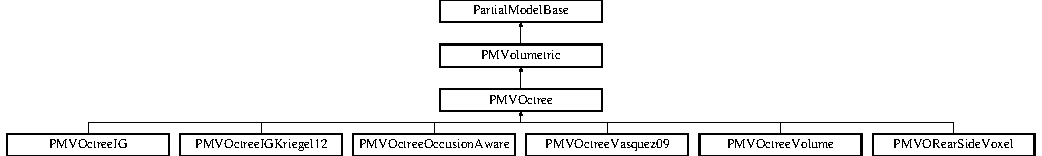
\includegraphics[height=2.097378cm]{classPMVOctree}
\end{center}
\end{figure}
\subsection*{Public Member Functions}
\begin{DoxyCompactItemize}
\item 
virtual float {\bfseries update\+With\+Scan} (std\+::string file\+\_\+name\+\_\+scan, std\+::string file\+\_\+name\+\_\+origin)\hypertarget{classPMVOctree_ae7dcde3f6d0186b480e4c466dc838069}{}\label{classPMVOctree_ae7dcde3f6d0186b480e4c466dc838069}

\item 
virtual bool {\bfseries save\+Partial\+Model} (std\+::string file\+\_\+name)\hypertarget{classPMVOctree_a9d43e80dbe4b31d2c8867d6044f89315}{}\label{classPMVOctree_a9d43e80dbe4b31d2c8867d6044f89315}

\item 
virtual bool {\bfseries load\+Partial\+Model} (std\+::string file\+\_\+name)\hypertarget{classPMVOctree_a05ea11ddb9ef9dc2f42bb3e12421178d}{}\label{classPMVOctree_a05ea11ddb9ef9dc2f42bb3e12421178d}

\item 
virtual int \hyperlink{classPMVOctree_a2f35ea94079904f2e336776cec14b234}{evaluate\+View} (\hyperlink{classViewStructure}{View\+Structure} \&v)
\item 
virtual long int \hyperlink{classPMVOctree_aea21d58041a90e416e35b1e30d8e4f2f}{read\+Rays} (std\+::string file\+\_\+address)
\item 
long int \hyperlink{classPMVOctree_ab94a5f29d9bab3fdf4b29211d7e8e2ed}{paint\+Voxels} (\hyperlink{classCOctreeVPL}{C\+Octree\+V\+PL} $\ast$octree)
\item 
long int \hyperlink{classPMVOctree_a6069af536fca552725d2c35b73f87329}{paint\+Voxels} ()
\item 
virtual bool {\bfseries init} ()\hypertarget{classPMVOctree_a0d9ee4ea4405227380ff8d2702194e65}{}\label{classPMVOctree_a0d9ee4ea4405227380ff8d2702194e65}

\item 
void \hyperlink{classPMVOctree_a12f82c34c03613a96023416be4f19016}{insert\+Free\+Space} (double x1, double y1, double z1, double x2, double y2, double z2)
\item 
virtual void \hyperlink{classPMVOctree_a774f55223acf795f52d3f73c8c9471cc}{save\+Object\+As\+RawT} (std\+::string file\+\_\+name)
\item 
virtual void \hyperlink{classPMVOctree_aca1c65f5363719f37247f80286a6154f}{save\+Object\+As\+Obst} (std\+::string file\+\_\+name)
\item 
virtual bool \hyperlink{classPMVOctree_aeafe9d9017283183e9d45824e2ef9c8a}{save\+Unknown\+Volume\+As\+Obst} (std\+::string file\+\_\+name)
\item 
virtual bool \hyperlink{classPMVOctree_a2d9c6839bb00a6c93129e34e1215fb9b}{save\+Unknown\+Volume\+As\+RawT} (std\+::string file\+\_\+name)
\item 
virtual bool {\bfseries save\+Visible\+Unknown} (std\+::string file\+\_\+name\+\_\+vertex, std\+::string file\+\_\+name\+\_\+normal)\hypertarget{classPMVOctree_a4bdf27fbd5933360a4dce4a45c1ff1a5}{}\label{classPMVOctree_a4bdf27fbd5933360a4dce4a45c1ff1a5}

\item 
virtual bool {\bfseries save\+Frontier\+Unknown} (std\+::string file\+\_\+name\+\_\+vertex, std\+::string file\+\_\+name\+\_\+normal)\hypertarget{classPMVOctree_ae311223977861d14ac9bc97f77194448}{}\label{classPMVOctree_ae311223977861d14ac9bc97f77194448}

\item 
virtual bool \hyperlink{classPMVOctree_a4a6e07836f0258cd32d5bcb89867ae03}{save\+Obstacle} (std\+::string file\+\_\+name)
\item 
virtual void {\bfseries get\+Occupied\+Triangles} (\hyperlink{classvpTriangleList}{vp\+Triangle\+List} \&tris)\hypertarget{classPMVOctree_a963e41d16ae7a3b37baf64e1c309e35f}{}\label{classPMVOctree_a963e41d16ae7a3b37baf64e1c309e35f}

\item 
virtual void {\bfseries get\+Unknown\+Triangles} (\hyperlink{classvpTriangleList}{vp\+Triangle\+List} \&tris)\hypertarget{classPMVOctree_a1e9af592a9b42e7330c34faa7fec748a}{}\label{classPMVOctree_a1e9af592a9b42e7330c34faa7fec748a}

\item 
virtual double \hyperlink{classPMVOctree_a55c27c46a523772761512e1f139802ba}{get\+Unknown\+Volume} ()
\end{DoxyCompactItemize}
\subsection*{Protected Member Functions}
\begin{DoxyCompactItemize}
\item 
virtual bool \hyperlink{classPMVOctree_a7f3ca384e40ac57446ec20d9acbefa92}{ray\+Tracing\+H\+TM} (boost\+::numeric\+::ublas\+::matrix$<$ double $>$ m, \hyperlink{classEvaluationResult}{Evaluation\+Result} \&result)
\item 
virtual bool {\bfseries registration\+Constraint} (\hyperlink{classEvaluationResult}{Evaluation\+Result} r)\hypertarget{classPMVOctree_a5fb49eeca15fa16a47d6568b592ae76d}{}\label{classPMVOctree_a5fb49eeca15fa16a47d6568b592ae76d}

\end{DoxyCompactItemize}
\subsection*{Protected Attributes}
\begin{DoxyCompactItemize}
\item 
\hyperlink{classCOctreeVPL}{C\+Octree\+V\+PL} $\ast$ \hyperlink{classPMVOctree_a922c0a5e617d067b2088372fdab2d9dd}{map}\hypertarget{classPMVOctree_a922c0a5e617d067b2088372fdab2d9dd}{}\label{classPMVOctree_a922c0a5e617d067b2088372fdab2d9dd}

\begin{DoxyCompactList}\small\item\em Octree representation. \end{DoxyCompactList}\end{DoxyCompactItemize}
\subsection*{Additional Inherited Members}


\subsection{Detailed Description}
Partial Model based on a probabilistic octree Reported in\+: Vasquez-\/\+Gomez, J. I., Sucar, L. E., \& Murrieta-\/\+Cid, R. (2017). View/state planning for three-\/dimensional object reconstruction under uncertainty. Autonomous Robots, 41(1), 89-\/109.

Initialization\+:
\begin{DoxyItemize}
\item Set config folder
\item Set data folder
\item init()
\item \hyperlink{classPMVOctree_aea21d58041a90e416e35b1e30d8e4f2f}{read\+Rays()};
\item set utility function 
\end{DoxyItemize}

\subsection{Member Function Documentation}
\index{P\+M\+V\+Octree@{P\+M\+V\+Octree}!evaluate\+View@{evaluate\+View}}
\index{evaluate\+View@{evaluate\+View}!P\+M\+V\+Octree@{P\+M\+V\+Octree}}
\subsubsection[{\texorpdfstring{evaluate\+View(\+View\+Structure \&v)}{evaluateView(ViewStructure &v)}}]{\setlength{\rightskip}{0pt plus 5cm}int P\+M\+V\+Octree\+::evaluate\+View (
\begin{DoxyParamCaption}
\item[{{\bf View\+Structure} \&}]{v}
\end{DoxyParamCaption}
)\hspace{0.3cm}{\ttfamily [virtual]}}\hypertarget{classPMVOctree_a2f35ea94079904f2e336776cec14b234}{}\label{classPMVOctree_a2f35ea94079904f2e336776cec14b234}
Evaluate the result of the raytracing 

Implements \hyperlink{classPartialModelBase}{Partial\+Model\+Base}.



Reimplemented in \hyperlink{classPMVORearSideVoxel_abfbe9be1007d7d7fe7434031c1d96ad1}{P\+M\+V\+O\+Rear\+Side\+Voxel}, and \hyperlink{classPMVOctreeVasquez09_accb4475c4387147aed552e9dc1172377}{P\+M\+V\+Octree\+Vasquez09}.

\index{P\+M\+V\+Octree@{P\+M\+V\+Octree}!get\+Unknown\+Volume@{get\+Unknown\+Volume}}
\index{get\+Unknown\+Volume@{get\+Unknown\+Volume}!P\+M\+V\+Octree@{P\+M\+V\+Octree}}
\subsubsection[{\texorpdfstring{get\+Unknown\+Volume()}{getUnknownVolume()}}]{\setlength{\rightskip}{0pt plus 5cm}double P\+M\+V\+Octree\+::get\+Unknown\+Volume (
\begin{DoxyParamCaption}
{}
\end{DoxyParamCaption}
)\hspace{0.3cm}{\ttfamily [virtual]}}\hypertarget{classPMVOctree_a55c27c46a523772761512e1f139802ba}{}\label{classPMVOctree_a55c27c46a523772761512e1f139802ba}
Returns an aproximation of the unknown volume; 

Implements \hyperlink{classPartialModelBase_a3dc1ffa43084246c6a79b5763025dc73}{Partial\+Model\+Base}.

\index{P\+M\+V\+Octree@{P\+M\+V\+Octree}!insert\+Free\+Space@{insert\+Free\+Space}}
\index{insert\+Free\+Space@{insert\+Free\+Space}!P\+M\+V\+Octree@{P\+M\+V\+Octree}}
\subsubsection[{\texorpdfstring{insert\+Free\+Space(double x1, double y1, double z1, double x2, double y2, double z2)}{insertFreeSpace(double x1, double y1, double z1, double x2, double y2, double z2)}}]{\setlength{\rightskip}{0pt plus 5cm}void P\+M\+V\+Octree\+::insert\+Free\+Space (
\begin{DoxyParamCaption}
\item[{double}]{x1, }
\item[{double}]{y1, }
\item[{double}]{z1, }
\item[{double}]{x2, }
\item[{double}]{y2, }
\item[{double}]{z2}
\end{DoxyParamCaption}
)}\hypertarget{classPMVOctree_a12f82c34c03613a96023416be4f19016}{}\label{classPMVOctree_a12f82c34c03613a96023416be4f19016}
Inserts a cube of free space given by two xtreme points \index{P\+M\+V\+Octree@{P\+M\+V\+Octree}!paint\+Voxels@{paint\+Voxels}}
\index{paint\+Voxels@{paint\+Voxels}!P\+M\+V\+Octree@{P\+M\+V\+Octree}}
\subsubsection[{\texorpdfstring{paint\+Voxels(\+C\+Octree\+V\+P\+L $\ast$octree)}{paintVoxels(COctreeVPL *octree)}}]{\setlength{\rightskip}{0pt plus 5cm}long int P\+M\+V\+Octree\+::paint\+Voxels (
\begin{DoxyParamCaption}
\item[{{\bf C\+Octree\+V\+PL} $\ast$}]{octree}
\end{DoxyParamCaption}
)}\hypertarget{classPMVOctree_ab94a5f29d9bab3fdf4b29211d7e8e2ed}{}\label{classPMVOctree_ab94a5f29d9bab3fdf4b29211d7e8e2ed}
Paints in blue occupied voxels that are inside the object capsule. Paints in orange unknown voxels \index{P\+M\+V\+Octree@{P\+M\+V\+Octree}!paint\+Voxels@{paint\+Voxels}}
\index{paint\+Voxels@{paint\+Voxels}!P\+M\+V\+Octree@{P\+M\+V\+Octree}}
\subsubsection[{\texorpdfstring{paint\+Voxels()}{paintVoxels()}}]{\setlength{\rightskip}{0pt plus 5cm}long int P\+M\+V\+Octree\+::paint\+Voxels (
\begin{DoxyParamCaption}
{}
\end{DoxyParamCaption}
)}\hypertarget{classPMVOctree_a6069af536fca552725d2c35b73f87329}{}\label{classPMVOctree_a6069af536fca552725d2c35b73f87329}
Paints in blue occupied voxels that are inside the object capsule. Paints in orange unknown voxels \index{P\+M\+V\+Octree@{P\+M\+V\+Octree}!ray\+Tracing\+H\+TM@{ray\+Tracing\+H\+TM}}
\index{ray\+Tracing\+H\+TM@{ray\+Tracing\+H\+TM}!P\+M\+V\+Octree@{P\+M\+V\+Octree}}
\subsubsection[{\texorpdfstring{ray\+Tracing\+H\+T\+M(boost\+::numeric\+::ublas\+::matrix$<$ double $>$ m, Evaluation\+Result \&result)}{rayTracingHTM(boost::numeric::ublas::matrix< double > m, EvaluationResult &result)}}]{\setlength{\rightskip}{0pt plus 5cm}bool P\+M\+V\+Octree\+::ray\+Tracing\+H\+TM (
\begin{DoxyParamCaption}
\item[{boost\+::numeric\+::ublas\+::matrix$<$ double $>$}]{m, }
\item[{{\bf Evaluation\+Result} \&}]{result}
\end{DoxyParamCaption}
)\hspace{0.3cm}{\ttfamily [protected]}, {\ttfamily [virtual]}}\hypertarget{classPMVOctree_a7f3ca384e40ac57446ec20d9acbefa92}{}\label{classPMVOctree_a7f3ca384e40ac57446ec20d9acbefa92}
Performs a ray tracing to gather how much voxels ware touched. It uses the translation of the H\+TM like origin of the ray tracing. Returns false if the origin is not free. 
\begin{DoxyParams}{Parameters}
{\em m} & \mbox{[}in\mbox{]} Homogenous transformation matrix. It will be applied to the sensor model \\
\hline
{\em n\+\_\+occupied} & \mbox{[}out\mbox{]} \\
\hline
{\em n\+\_\+unknown} & \mbox{[}out\mbox{]} \\
\hline
\end{DoxyParams}
The ray is rotated and traslated by the rotation matrix 

Reimplemented in \hyperlink{classPMVORearSideVoxel_afd9b08599913cf32cbc315cb210f4924}{P\+M\+V\+O\+Rear\+Side\+Voxel}, and \hyperlink{classPMVOctreeVolume_a4c4a6581a0c693feab63de557861390d}{P\+M\+V\+Octree\+Volume}.

\index{P\+M\+V\+Octree@{P\+M\+V\+Octree}!read\+Rays@{read\+Rays}}
\index{read\+Rays@{read\+Rays}!P\+M\+V\+Octree@{P\+M\+V\+Octree}}
\subsubsection[{\texorpdfstring{read\+Rays(std\+::string file\+\_\+address)}{readRays(std::string file_address)}}]{\setlength{\rightskip}{0pt plus 5cm}long int P\+M\+V\+Octree\+::read\+Rays (
\begin{DoxyParamCaption}
\item[{std\+::string}]{file\+\_\+address}
\end{DoxyParamCaption}
)\hspace{0.3cm}{\ttfamily [virtual]}}\hypertarget{classPMVOctree_aea21d58041a90e416e35b1e30d8e4f2f}{}\label{classPMVOctree_aea21d58041a90e416e35b1e30d8e4f2f}
Reads the rays (directions) thought by the sensor They are stored at rays with the notation \mbox{[}x, y, z, 1\mbox{]}$^\wedge$T The 1 is added to perform matrix multiplications by a H\+TM 

Implements \hyperlink{classPartialModelBase_a645f1e68e3e29419522c3ef10ee05d05}{Partial\+Model\+Base}.

\index{P\+M\+V\+Octree@{P\+M\+V\+Octree}!save\+Object\+As\+Obst@{save\+Object\+As\+Obst}}
\index{save\+Object\+As\+Obst@{save\+Object\+As\+Obst}!P\+M\+V\+Octree@{P\+M\+V\+Octree}}
\subsubsection[{\texorpdfstring{save\+Object\+As\+Obst(std\+::string file\+\_\+name)}{saveObjectAsObst(std::string file_name)}}]{\setlength{\rightskip}{0pt plus 5cm}void P\+M\+V\+Octree\+::save\+Object\+As\+Obst (
\begin{DoxyParamCaption}
\item[{std\+::string}]{file\+\_\+name}
\end{DoxyParamCaption}
)\hspace{0.3cm}{\ttfamily [virtual]}}\hypertarget{classPMVOctree_aca1c65f5363719f37247f80286a6154f}{}\label{classPMVOctree_aca1c65f5363719f37247f80286a6154f}
Saves the occupied and uknown voxels inside the object bouding box as a list of triangles. 

Implements \hyperlink{classPartialModelBase_a994da889db902ef5948d9db48609d00b}{Partial\+Model\+Base}.

\index{P\+M\+V\+Octree@{P\+M\+V\+Octree}!save\+Object\+As\+RawT@{save\+Object\+As\+RawT}}
\index{save\+Object\+As\+RawT@{save\+Object\+As\+RawT}!P\+M\+V\+Octree@{P\+M\+V\+Octree}}
\subsubsection[{\texorpdfstring{save\+Object\+As\+Raw\+T(std\+::string file\+\_\+name)}{saveObjectAsRawT(std::string file_name)}}]{\setlength{\rightskip}{0pt plus 5cm}void P\+M\+V\+Octree\+::save\+Object\+As\+RawT (
\begin{DoxyParamCaption}
\item[{std\+::string}]{file\+\_\+name}
\end{DoxyParamCaption}
)\hspace{0.3cm}{\ttfamily [virtual]}}\hypertarget{classPMVOctree_a774f55223acf795f52d3f73c8c9471cc}{}\label{classPMVOctree_a774f55223acf795f52d3f73c8c9471cc}
Saves the occupied and uknown voxels inside the object bouding box as a list of triangles. 

Implements \hyperlink{classPartialModelBase_a193634a1ffbc43b60164dae988204d9e}{Partial\+Model\+Base}.

\index{P\+M\+V\+Octree@{P\+M\+V\+Octree}!save\+Obstacle@{save\+Obstacle}}
\index{save\+Obstacle@{save\+Obstacle}!P\+M\+V\+Octree@{P\+M\+V\+Octree}}
\subsubsection[{\texorpdfstring{save\+Obstacle(std\+::string file\+\_\+name)}{saveObstacle(std::string file_name)}}]{\setlength{\rightskip}{0pt plus 5cm}bool P\+M\+V\+Octree\+::save\+Obstacle (
\begin{DoxyParamCaption}
\item[{std\+::string}]{file\+\_\+name}
\end{DoxyParamCaption}
)\hspace{0.3cm}{\ttfamily [virtual]}}\hypertarget{classPMVOctree_a4a6e07836f0258cd32d5bcb89867ae03}{}\label{classPMVOctree_a4a6e07836f0258cd32d5bcb89867ae03}
Saves the occupied and unknown voxels as Obs 

Implements \hyperlink{classPartialModelBase_ab41193a2a697dcf0d7d416cb35836458}{Partial\+Model\+Base}.

\index{P\+M\+V\+Octree@{P\+M\+V\+Octree}!save\+Unknown\+Volume\+As\+Obst@{save\+Unknown\+Volume\+As\+Obst}}
\index{save\+Unknown\+Volume\+As\+Obst@{save\+Unknown\+Volume\+As\+Obst}!P\+M\+V\+Octree@{P\+M\+V\+Octree}}
\subsubsection[{\texorpdfstring{save\+Unknown\+Volume\+As\+Obst(std\+::string file\+\_\+name)}{saveUnknownVolumeAsObst(std::string file_name)}}]{\setlength{\rightskip}{0pt plus 5cm}bool P\+M\+V\+Octree\+::save\+Unknown\+Volume\+As\+Obst (
\begin{DoxyParamCaption}
\item[{std\+::string}]{file\+\_\+name}
\end{DoxyParamCaption}
)\hspace{0.3cm}{\ttfamily [virtual]}}\hypertarget{classPMVOctree_aeafe9d9017283183e9d45824e2ef9c8a}{}\label{classPMVOctree_aeafe9d9017283183e9d45824e2ef9c8a}
used for motion planning 

Implements \hyperlink{classPartialModelBase_a6b5f29ca5354d246ec08af21f764552e}{Partial\+Model\+Base}.

\index{P\+M\+V\+Octree@{P\+M\+V\+Octree}!save\+Unknown\+Volume\+As\+RawT@{save\+Unknown\+Volume\+As\+RawT}}
\index{save\+Unknown\+Volume\+As\+RawT@{save\+Unknown\+Volume\+As\+RawT}!P\+M\+V\+Octree@{P\+M\+V\+Octree}}
\subsubsection[{\texorpdfstring{save\+Unknown\+Volume\+As\+Raw\+T(std\+::string file\+\_\+name)}{saveUnknownVolumeAsRawT(std::string file_name)}}]{\setlength{\rightskip}{0pt plus 5cm}bool P\+M\+V\+Octree\+::save\+Unknown\+Volume\+As\+RawT (
\begin{DoxyParamCaption}
\item[{std\+::string}]{file\+\_\+name}
\end{DoxyParamCaption}
)\hspace{0.3cm}{\ttfamily [virtual]}}\hypertarget{classPMVOctree_a2d9c6839bb00a6c93129e34e1215fb9b}{}\label{classPMVOctree_a2d9c6839bb00a6c93129e34e1215fb9b}
Saves the unknown voxels inside the object bouding box as a list of triangles. 

Implements \hyperlink{classPartialModelBase_a2f0c03925d1afc098dede157d0876ee3}{Partial\+Model\+Base}.



The documentation for this class was generated from the following files\+:\begin{DoxyCompactItemize}
\item 
partialmodel/pmvoctree.\+h\item 
partialmodel/pmvoctree.\+cpp\end{DoxyCompactItemize}

\hypertarget{classPMVOctreeIG}{}\section{P\+M\+V\+Octree\+IG Class Reference}
\label{classPMVOctreeIG}\index{P\+M\+V\+Octree\+IG@{P\+M\+V\+Octree\+IG}}


{\ttfamily \#include $<$pmvoctreeig.\+h$>$}

Inheritance diagram for P\+M\+V\+Octree\+IG\+:\begin{figure}[H]
\begin{center}
\leavevmode
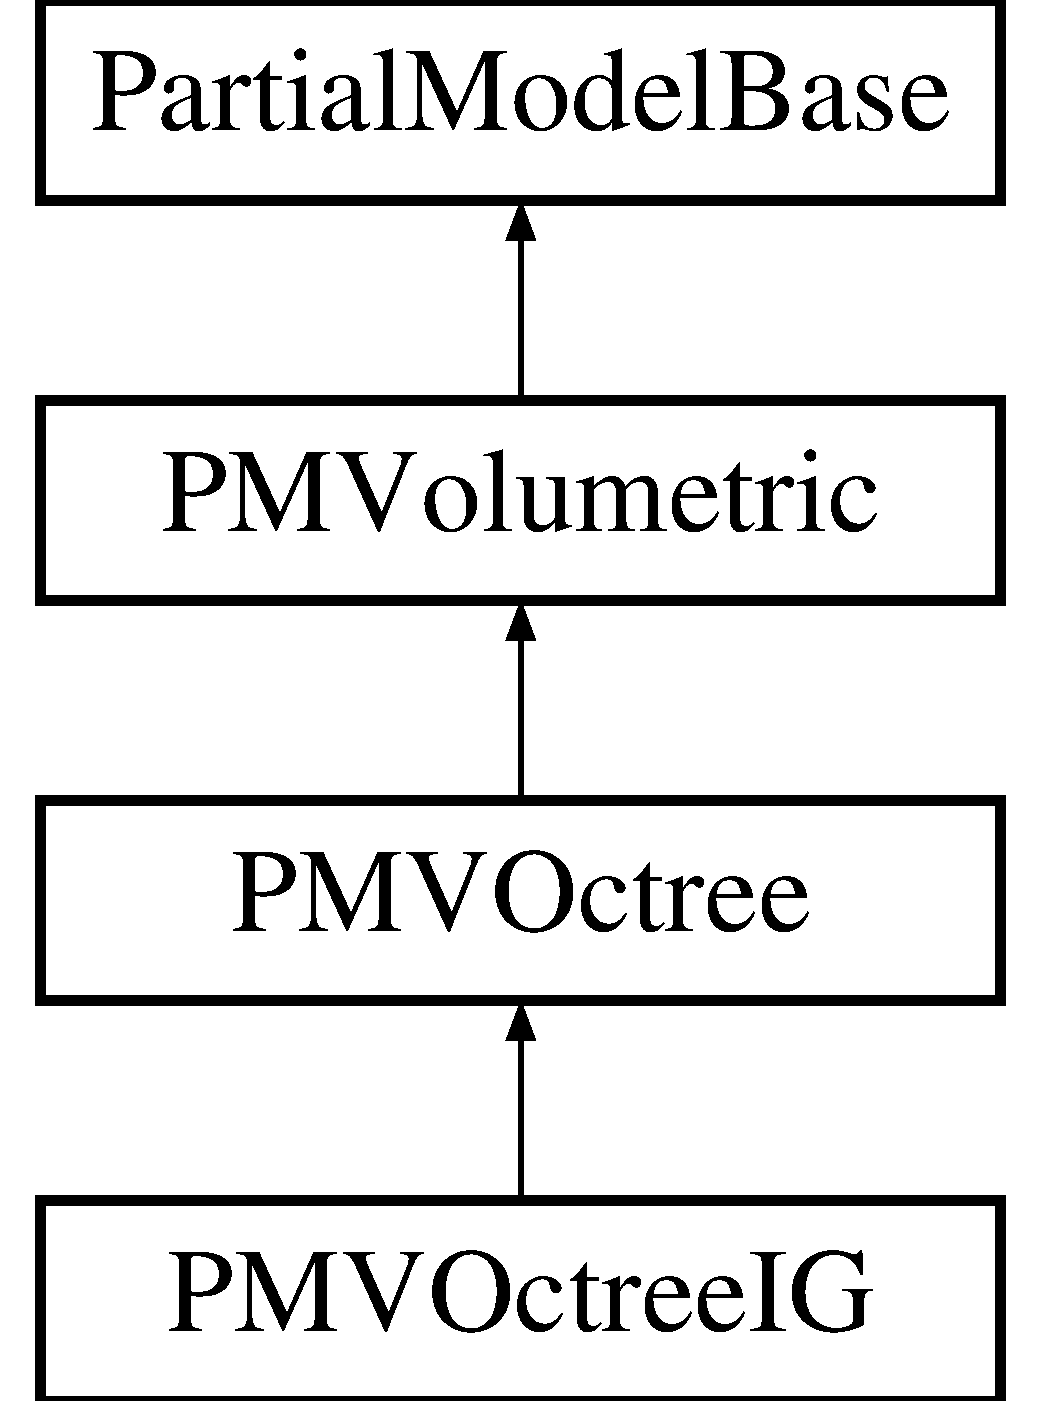
\includegraphics[height=4.000000cm]{classPMVOctreeIG}
\end{center}
\end{figure}
\subsection*{Public Member Functions}
\begin{DoxyCompactItemize}
\item 
virtual int {\bfseries evaluate\+View} (\hyperlink{classViewStructure}{View\+Structure} \&v)\hypertarget{classPMVOctreeIG_a065d48a94b4343325d08bb55ffc0d332}{}\label{classPMVOctreeIG_a065d48a94b4343325d08bb55ffc0d332}

\item 
virtual float {\bfseries update\+With\+Scan} (std\+::string file\+\_\+name\+\_\+scan, std\+::string file\+\_\+name\+\_\+origin)\hypertarget{classPMVOctreeIG_ae5f60e009d2c0f71115e583dcdafdd96}{}\label{classPMVOctreeIG_ae5f60e009d2c0f71115e583dcdafdd96}

\end{DoxyCompactItemize}
\subsection*{Protected Member Functions}
\begin{DoxyCompactItemize}
\item 
double \hyperlink{classPMVOctreeIG_a752fb0c18f988c4d8a0653ce8b850a44}{ray\+Tracing\+H\+T\+M\+IG} (boost\+::numeric\+::ublas\+::matrix$<$ double $>$ m, \hyperlink{classEvaluationResult}{Evaluation\+Result} \&result)
\end{DoxyCompactItemize}
\subsection*{Additional Inherited Members}


\subsection{Detailed Description}
Partial Model based on a probabilistic octree Frustum Information Gain Reported in\+: I\+R\+O\+S17 submitted

Initialization\+:
\begin{DoxyItemize}
\item Set config folder
\item Set data folder
\item init()
\item \hyperlink{classPMVOctree_aea21d58041a90e416e35b1e30d8e4f2f}{read\+Rays()};
\item set utility function 
\end{DoxyItemize}

\subsection{Member Function Documentation}
\index{P\+M\+V\+Octree\+IG@{P\+M\+V\+Octree\+IG}!ray\+Tracing\+H\+T\+M\+IG@{ray\+Tracing\+H\+T\+M\+IG}}
\index{ray\+Tracing\+H\+T\+M\+IG@{ray\+Tracing\+H\+T\+M\+IG}!P\+M\+V\+Octree\+IG@{P\+M\+V\+Octree\+IG}}
\subsubsection[{\texorpdfstring{ray\+Tracing\+H\+T\+M\+I\+G(boost\+::numeric\+::ublas\+::matrix$<$ double $>$ m, Evaluation\+Result \&result)}{rayTracingHTMIG(boost::numeric::ublas::matrix< double > m, EvaluationResult &result)}}]{\setlength{\rightskip}{0pt plus 5cm}double P\+M\+V\+Octree\+I\+G\+::ray\+Tracing\+H\+T\+M\+IG (
\begin{DoxyParamCaption}
\item[{boost\+::numeric\+::ublas\+::matrix$<$ double $>$}]{m, }
\item[{{\bf Evaluation\+Result} \&}]{result}
\end{DoxyParamCaption}
)\hspace{0.3cm}{\ttfamily [protected]}}\hypertarget{classPMVOctreeIG_a752fb0c18f988c4d8a0653ce8b850a44}{}\label{classPMVOctreeIG_a752fb0c18f988c4d8a0653ce8b850a44}
The ray is rotated and traslated by the rotation matrix 

The documentation for this class was generated from the following files\+:\begin{DoxyCompactItemize}
\item 
partialmodel/pmvoctreeig.\+h\item 
partialmodel/pmvoctreeig.\+cpp\end{DoxyCompactItemize}

\hypertarget{classPMVOctreeIGKriegel12}{}\section{P\+M\+V\+Octree\+I\+G\+Kriegel12 Class Reference}
\label{classPMVOctreeIGKriegel12}\index{P\+M\+V\+Octree\+I\+G\+Kriegel12@{P\+M\+V\+Octree\+I\+G\+Kriegel12}}


{\ttfamily \#include $<$pmvoctreeigkriegel12.\+h$>$}

Inheritance diagram for P\+M\+V\+Octree\+I\+G\+Kriegel12\+:\begin{figure}[H]
\begin{center}
\leavevmode
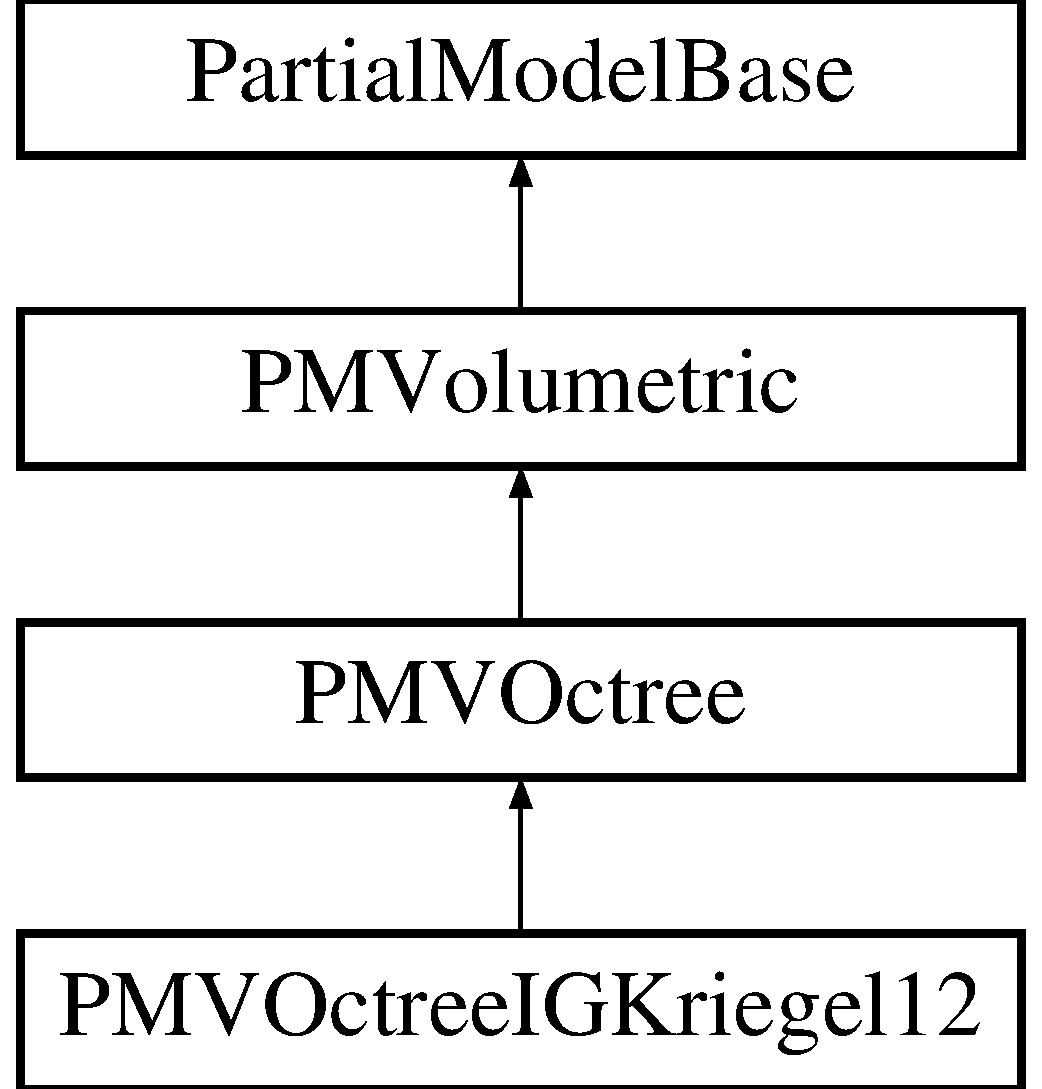
\includegraphics[height=4.000000cm]{classPMVOctreeIGKriegel12}
\end{center}
\end{figure}
\subsection*{Public Member Functions}
\begin{DoxyCompactItemize}
\item 
virtual bool {\bfseries init} ()\hypertarget{classPMVOctreeIGKriegel12_af7acc855c6276f22fe7c8736cfd2ed82}{}\label{classPMVOctreeIGKriegel12_af7acc855c6276f22fe7c8736cfd2ed82}

\item 
virtual int {\bfseries evaluate\+View} (\hyperlink{classViewStructure}{View\+Structure} \&v)\hypertarget{classPMVOctreeIGKriegel12_a8744c422b2a9b11859560aa98e8d2f7d}{}\label{classPMVOctreeIGKriegel12_a8744c422b2a9b11859560aa98e8d2f7d}

\item 
virtual float {\bfseries update\+With\+Scan} (std\+::string file\+\_\+name\+\_\+scan, std\+::string file\+\_\+name\+\_\+origin)\hypertarget{classPMVOctreeIGKriegel12_aa8720c9fedbfab494aa8cb21848c6b54}{}\label{classPMVOctreeIGKriegel12_aa8720c9fedbfab494aa8cb21848c6b54}

\end{DoxyCompactItemize}
\subsection*{Protected Member Functions}
\begin{DoxyCompactItemize}
\item 
double \hyperlink{classPMVOctreeIGKriegel12_a9020231b50f8520fea577e41c5d0a44c}{ray\+Tracing\+H\+T\+M\+I\+G\+Kriegel} (boost\+::numeric\+::ublas\+::matrix$<$ double $>$ m, \hyperlink{classEvaluationResult}{Evaluation\+Result} \&result)
\end{DoxyCompactItemize}
\subsection*{Additional Inherited Members}


\subsection{Detailed Description}
Partial Model based on a probabilistic octree Reported in\+: Kriegel 12

Initialization\+:
\begin{DoxyItemize}
\item Set config folder
\item Set data folder
\item init()
\item \hyperlink{classPMVOctree_aea21d58041a90e416e35b1e30d8e4f2f}{read\+Rays()};
\item set utility function
\end{DoxyItemize}

Implementation status\+: ok Testing status\+: n/a 

\subsection{Member Function Documentation}
\index{P\+M\+V\+Octree\+I\+G\+Kriegel12@{P\+M\+V\+Octree\+I\+G\+Kriegel12}!ray\+Tracing\+H\+T\+M\+I\+G\+Kriegel@{ray\+Tracing\+H\+T\+M\+I\+G\+Kriegel}}
\index{ray\+Tracing\+H\+T\+M\+I\+G\+Kriegel@{ray\+Tracing\+H\+T\+M\+I\+G\+Kriegel}!P\+M\+V\+Octree\+I\+G\+Kriegel12@{P\+M\+V\+Octree\+I\+G\+Kriegel12}}
\subsubsection[{\texorpdfstring{ray\+Tracing\+H\+T\+M\+I\+G\+Kriegel(boost\+::numeric\+::ublas\+::matrix$<$ double $>$ m, Evaluation\+Result \&result)}{rayTracingHTMIGKriegel(boost::numeric::ublas::matrix< double > m, EvaluationResult &result)}}]{\setlength{\rightskip}{0pt plus 5cm}double P\+M\+V\+Octree\+I\+G\+Kriegel12\+::ray\+Tracing\+H\+T\+M\+I\+G\+Kriegel (
\begin{DoxyParamCaption}
\item[{boost\+::numeric\+::ublas\+::matrix$<$ double $>$}]{m, }
\item[{{\bf Evaluation\+Result} \&}]{result}
\end{DoxyParamCaption}
)\hspace{0.3cm}{\ttfamily [protected]}}\hypertarget{classPMVOctreeIGKriegel12_a9020231b50f8520fea577e41c5d0a44c}{}\label{classPMVOctreeIGKriegel12_a9020231b50f8520fea577e41c5d0a44c}
The ray is rotated and traslated by the rotation matrix 

The documentation for this class was generated from the following files\+:\begin{DoxyCompactItemize}
\item 
partialmodel/pmvoctreeigkriegel12.\+h\item 
partialmodel/pmvoctreeigkriegel12.\+cpp\end{DoxyCompactItemize}

\hypertarget{classPMVOctreeOccusionAware}{}\section{P\+M\+V\+Octree\+Occusion\+Aware Class Reference}
\label{classPMVOctreeOccusionAware}\index{P\+M\+V\+Octree\+Occusion\+Aware@{P\+M\+V\+Octree\+Occusion\+Aware}}
Inheritance diagram for P\+M\+V\+Octree\+Occusion\+Aware\+:\begin{figure}[H]
\begin{center}
\leavevmode
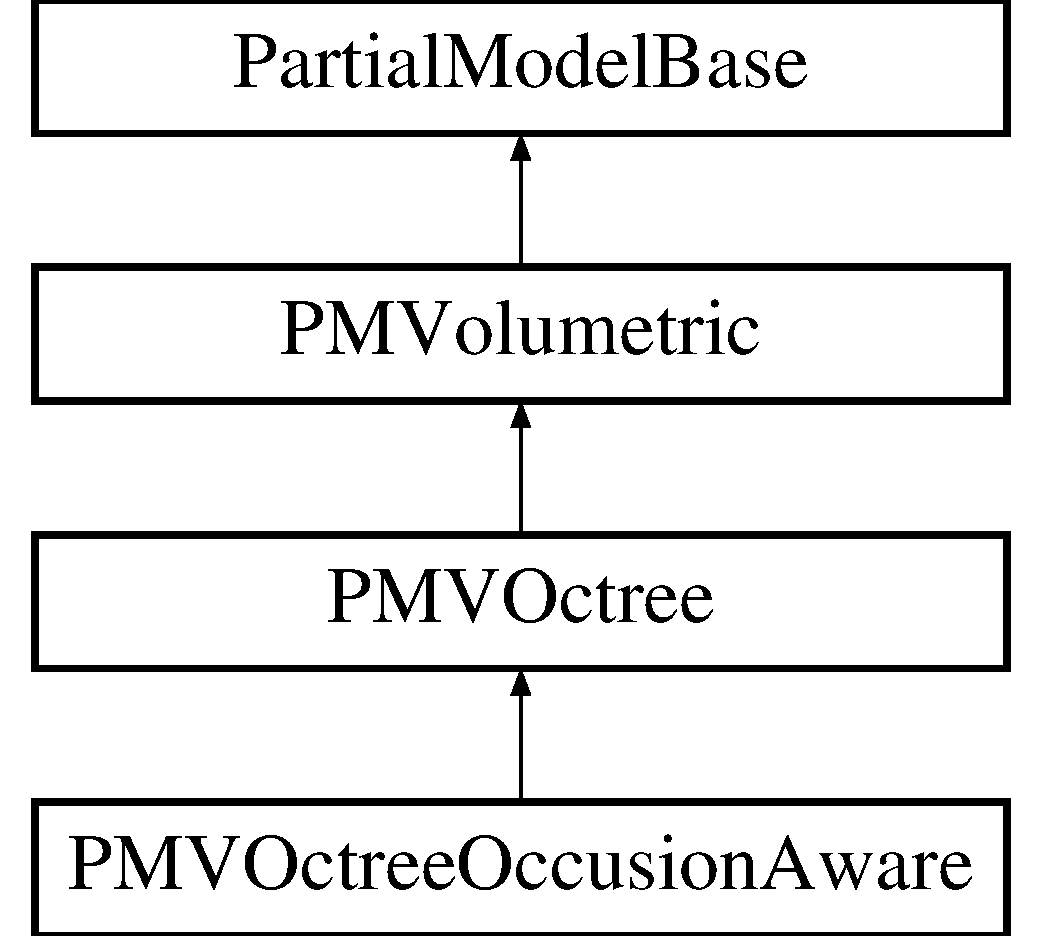
\includegraphics[height=4.000000cm]{classPMVOctreeOccusionAware}
\end{center}
\end{figure}
\subsection*{Public Member Functions}
\begin{DoxyCompactItemize}
\item 
virtual bool {\bfseries init} ()\hypertarget{classPMVOctreeOccusionAware_ae561f09096386b5ef6ba2ea706624a3a}{}\label{classPMVOctreeOccusionAware_ae561f09096386b5ef6ba2ea706624a3a}

\item 
virtual int {\bfseries evaluate\+View} (\hyperlink{classViewStructure}{View\+Structure} \&v)\hypertarget{classPMVOctreeOccusionAware_a8c8057b9b19acf6270d73beac3cebe0b}{}\label{classPMVOctreeOccusionAware_a8c8057b9b19acf6270d73beac3cebe0b}

\end{DoxyCompactItemize}
\subsection*{Additional Inherited Members}


The documentation for this class was generated from the following files\+:\begin{DoxyCompactItemize}
\item 
partialmodel/pmvoctreeoccusionaware.\+h\item 
partialmodel/pmvoctreeoccusionaware.\+cpp\end{DoxyCompactItemize}

\hypertarget{classPMVOctreeVasquez09}{}\section{P\+M\+V\+Octree\+Vasquez09 Class Reference}
\label{classPMVOctreeVasquez09}\index{P\+M\+V\+Octree\+Vasquez09@{P\+M\+V\+Octree\+Vasquez09}}
Inheritance diagram for P\+M\+V\+Octree\+Vasquez09\+:\begin{figure}[H]
\begin{center}
\leavevmode
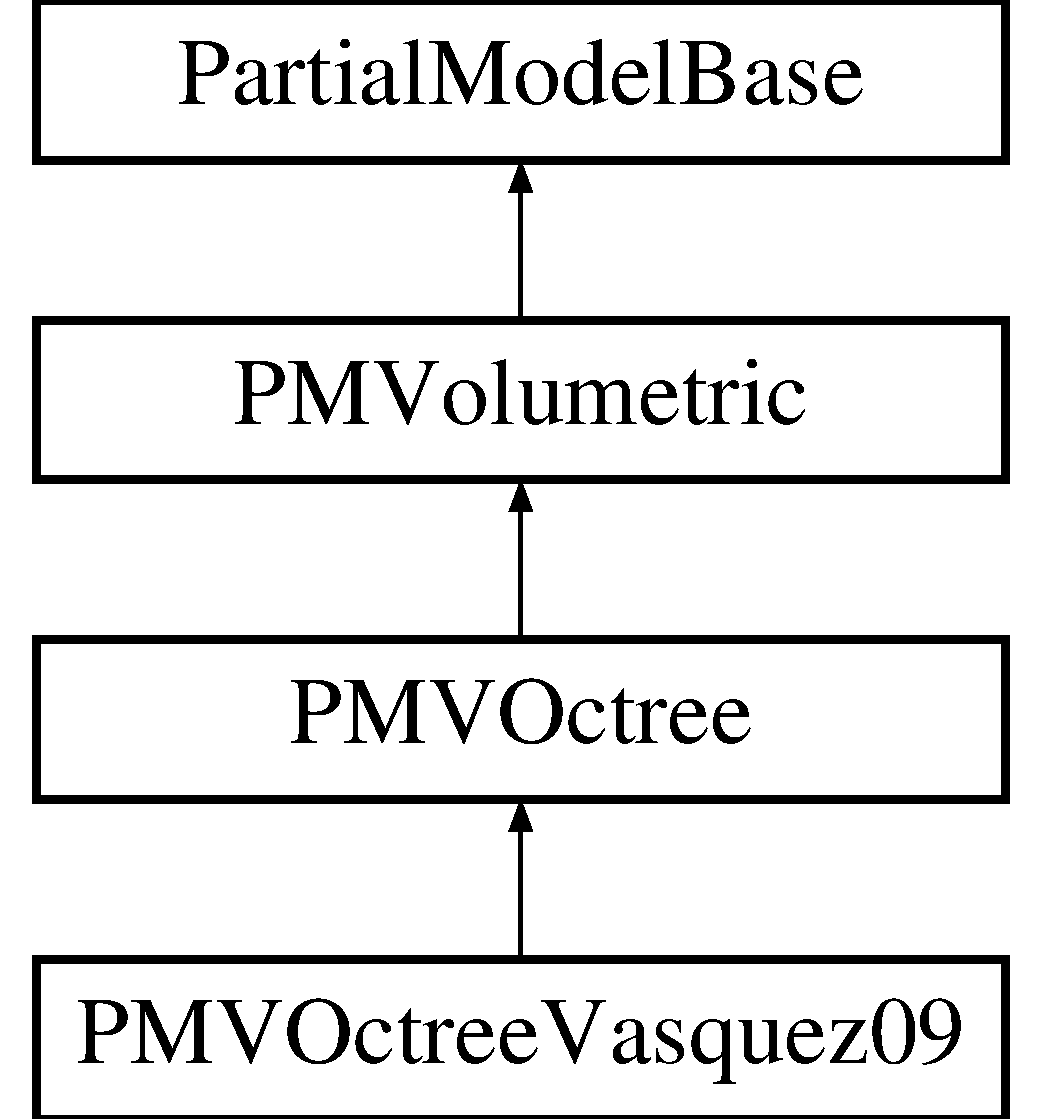
\includegraphics[height=4.000000cm]{classPMVOctreeVasquez09}
\end{center}
\end{figure}
\subsection*{Public Member Functions}
\begin{DoxyCompactItemize}
\item 
{\bfseries P\+M\+V\+Octree\+Vasquez09} (double alpha\+Occupied, double alpha\+Unknown)\hypertarget{classPMVOctreeVasquez09_a02767ba91cadb9e4f5ebb18697835af9}{}\label{classPMVOctreeVasquez09_a02767ba91cadb9e4f5ebb18697835af9}

\item 
virtual int \hyperlink{classPMVOctreeVasquez09_accb4475c4387147aed552e9dc1172377}{evaluate\+View} (\hyperlink{classViewStructure}{View\+Structure} \&v)
\end{DoxyCompactItemize}
\subsection*{Protected Attributes}
\begin{DoxyCompactItemize}
\item 
double {\bfseries alpha\+\_\+occupied}\hypertarget{classPMVOctreeVasquez09_ac107af7f792a5b0b4d81400a57c3af7c}{}\label{classPMVOctreeVasquez09_ac107af7f792a5b0b4d81400a57c3af7c}

\item 
double {\bfseries alpha\+\_\+unknown}\hypertarget{classPMVOctreeVasquez09_a4e6610193639eeee015d7019e1805874}{}\label{classPMVOctreeVasquez09_a4e6610193639eeee015d7019e1805874}

\end{DoxyCompactItemize}
\subsection*{Additional Inherited Members}


\subsection{Member Function Documentation}
\index{P\+M\+V\+Octree\+Vasquez09@{P\+M\+V\+Octree\+Vasquez09}!evaluate\+View@{evaluate\+View}}
\index{evaluate\+View@{evaluate\+View}!P\+M\+V\+Octree\+Vasquez09@{P\+M\+V\+Octree\+Vasquez09}}
\subsubsection[{\texorpdfstring{evaluate\+View(\+View\+Structure \&v)}{evaluateView(ViewStructure &v)}}]{\setlength{\rightskip}{0pt plus 5cm}int P\+M\+V\+Octree\+Vasquez09\+::evaluate\+View (
\begin{DoxyParamCaption}
\item[{{\bf View\+Structure} \&}]{v}
\end{DoxyParamCaption}
)\hspace{0.3cm}{\ttfamily [virtual]}}\hypertarget{classPMVOctreeVasquez09_accb4475c4387147aed552e9dc1172377}{}\label{classPMVOctreeVasquez09_accb4475c4387147aed552e9dc1172377}
Evaluate the result of the raytracing 

Reimplemented from \hyperlink{classPMVOctree_a2f35ea94079904f2e336776cec14b234}{P\+M\+V\+Octree}.



The documentation for this class was generated from the following files\+:\begin{DoxyCompactItemize}
\item 
partialmodel/pmvoctreevasquez09.\+h\item 
partialmodel/pmvoctreevasquez09.\+cpp\end{DoxyCompactItemize}

\hypertarget{classPMVOctreeVolume}{}\section{P\+M\+V\+Octree\+Volume Class Reference}
\label{classPMVOctreeVolume}\index{P\+M\+V\+Octree\+Volume@{P\+M\+V\+Octree\+Volume}}
Inheritance diagram for P\+M\+V\+Octree\+Volume\+:\begin{figure}[H]
\begin{center}
\leavevmode
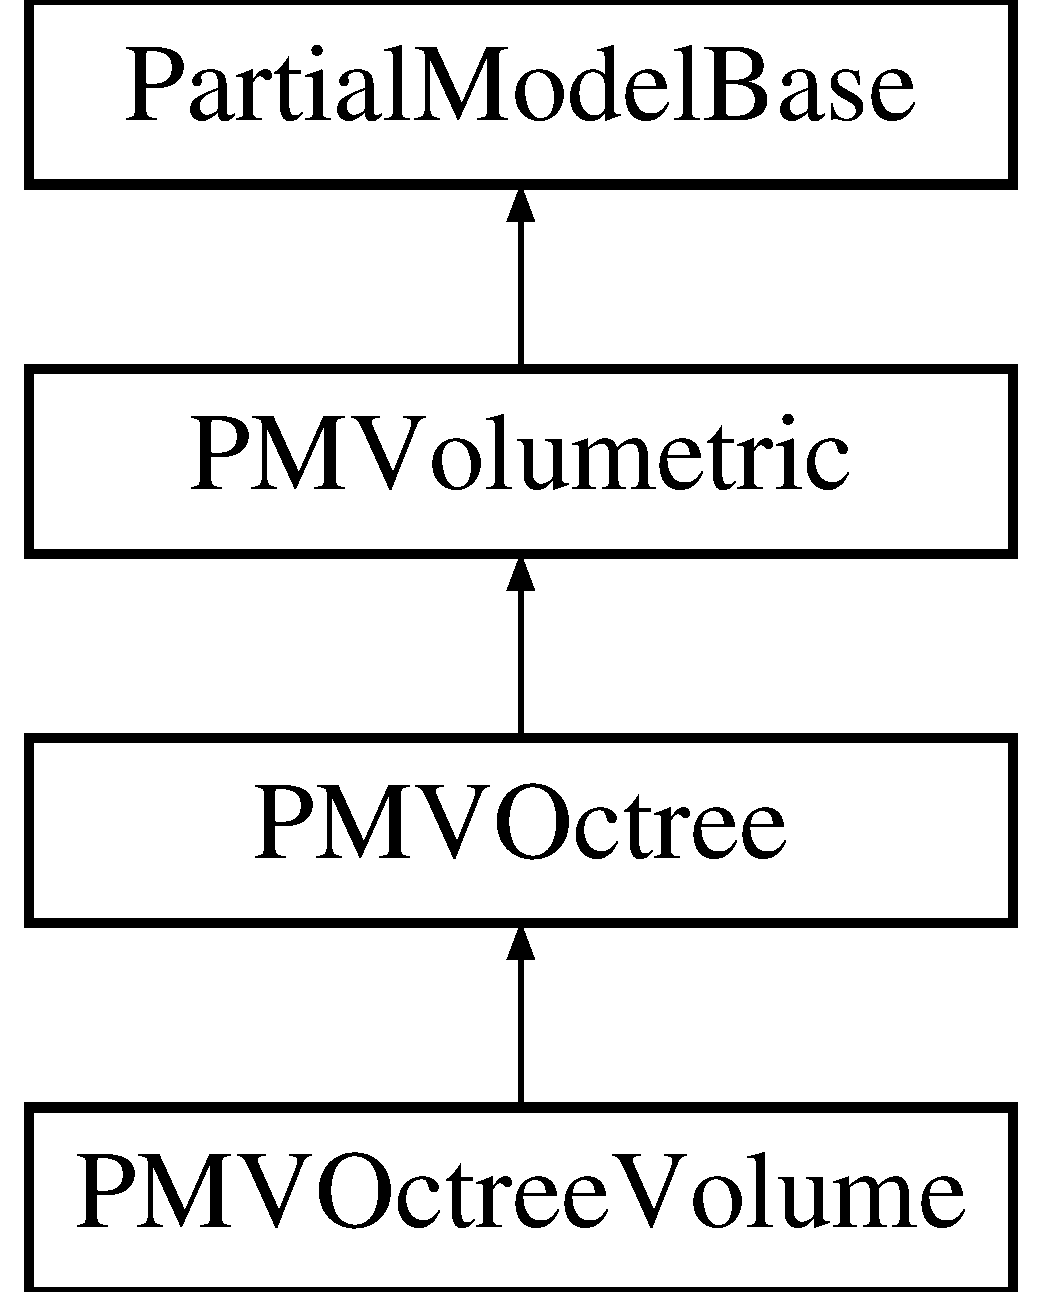
\includegraphics[height=4.000000cm]{classPMVOctreeVolume}
\end{center}
\end{figure}
\subsection*{Protected Member Functions}
\begin{DoxyCompactItemize}
\item 
bool \hyperlink{classPMVOctreeVolume_a4c4a6581a0c693feab63de557861390d}{ray\+Tracing\+H\+TM} (boost\+::numeric\+::ublas\+::matrix$<$ double $>$ m, \hyperlink{classEvaluationResult}{Evaluation\+Result} \&result)
\end{DoxyCompactItemize}
\subsection*{Additional Inherited Members}


\subsection{Member Function Documentation}
\index{P\+M\+V\+Octree\+Volume@{P\+M\+V\+Octree\+Volume}!ray\+Tracing\+H\+TM@{ray\+Tracing\+H\+TM}}
\index{ray\+Tracing\+H\+TM@{ray\+Tracing\+H\+TM}!P\+M\+V\+Octree\+Volume@{P\+M\+V\+Octree\+Volume}}
\subsubsection[{\texorpdfstring{ray\+Tracing\+H\+T\+M(boost\+::numeric\+::ublas\+::matrix$<$ double $>$ m, Evaluation\+Result \&result)}{rayTracingHTM(boost::numeric::ublas::matrix< double > m, EvaluationResult &result)}}]{\setlength{\rightskip}{0pt plus 5cm}bool P\+M\+V\+Octree\+Volume\+::ray\+Tracing\+H\+TM (
\begin{DoxyParamCaption}
\item[{boost\+::numeric\+::ublas\+::matrix$<$ double $>$}]{m, }
\item[{{\bf Evaluation\+Result} \&}]{result}
\end{DoxyParamCaption}
)\hspace{0.3cm}{\ttfamily [protected]}, {\ttfamily [virtual]}}\hypertarget{classPMVOctreeVolume_a4c4a6581a0c693feab63de557861390d}{}\label{classPMVOctreeVolume_a4c4a6581a0c693feab63de557861390d}
Performs a ray tracing to gather how much voxels ware touched. It uses the translation of the H\+TM like origin of the ray tracing. Returns false if the origin is not free. 
\begin{DoxyParams}{Parameters}
{\em m} & \mbox{[}in\mbox{]} Homogenous transformation matrix. It will be applied to the sensor model \\
\hline
{\em n\+\_\+occupied} & \mbox{[}out\mbox{]} \\
\hline
{\em n\+\_\+unknown} & \mbox{[}out\mbox{]} \\
\hline
\end{DoxyParams}
The ray is rotated and traslated by the rotation matrix 

Reimplemented from \hyperlink{classPMVOctree_a7f3ca384e40ac57446ec20d9acbefa92}{P\+M\+V\+Octree}.



The documentation for this class was generated from the following files\+:\begin{DoxyCompactItemize}
\item 
partialmodel/pmvoctreevolume.\+h\item 
partialmodel/pmvoctreevolume.\+cpp\end{DoxyCompactItemize}

\hypertarget{classPMVolumetric}{}\section{P\+M\+Volumetric Class Reference}
\label{classPMVolumetric}\index{P\+M\+Volumetric@{P\+M\+Volumetric}}


{\ttfamily \#include $<$pmvolumetric.\+h$>$}

Inheritance diagram for P\+M\+Volumetric\+:\begin{figure}[H]
\begin{center}
\leavevmode
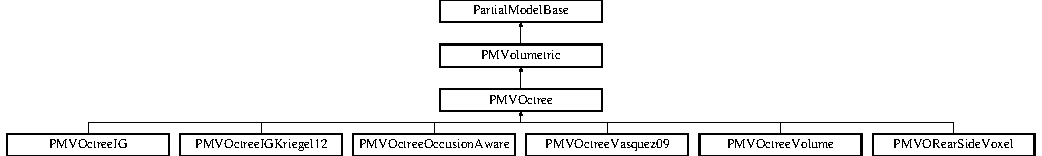
\includegraphics[height=2.097378cm]{classPMVolumetric}
\end{center}
\end{figure}
\subsection*{Public Member Functions}
\begin{DoxyCompactItemize}
\item 
virtual bool \hyperlink{classPMVolumetric_a6995737fe93356953555dc298f3fc2f9}{stop\+Criteria\+Reached} ()
\item 
virtual bool {\bfseries init} ()\hypertarget{classPMVolumetric_a429e9e6f82c5ef158b4732ae9252faaa}{}\label{classPMVolumetric_a429e9e6f82c5ef158b4732ae9252faaa}

\item 
virtual bool \hyperlink{classPMVolumetric_a1d5d45ef61e7741f322711e8396cd7ac}{collision\+Free} (float x, float y, float z)
\item 
virtual void {\bfseries save\+Evaluations} ()\hypertarget{classPMVolumetric_ad267f345bb318517b760d7fb7cfefcc1}{}\label{classPMVolumetric_ad267f345bb318517b760d7fb7cfefcc1}

\item 
void \hyperlink{classPMVolumetric_a8ca19a4a30b6a4991314b032cde35265}{set\+Minimun\+Number\+Of\+Unmark\+Voxels} (int n)
\item 
virtual bool {\bfseries save\+Visible\+Unknown} (std\+::string file\+\_\+name\+\_\+vertex, std\+::string file\+\_\+name\+\_\+normal)=0\hypertarget{classPMVolumetric_aede738844f4e5ccc30aece6358263160}{}\label{classPMVolumetric_aede738844f4e5ccc30aece6358263160}

\end{DoxyCompactItemize}
\subsection*{Protected Member Functions}
\begin{DoxyCompactItemize}
\item 
void \hyperlink{classPMVolumetric_a2eb41f090c07341c0667fd2cb760722a}{get\+Voxel\+Vertices} (point3d\+\_\+list \&vertices, const point3d center, const double resolution)
\item 
void \hyperlink{classPMVolumetric_a9aedd06e356c9fe46e6287a3b2361669}{get\+Triangles\+Of\+Voxel} (\hyperlink{classvpTriangleList}{vp\+Triangle\+List} \&tris, const point3d center, const double resolution)
\end{DoxyCompactItemize}
\subsection*{Protected Attributes}
\begin{DoxyCompactItemize}
\item 
std\+::vector$<$ point3d $>$ {\bfseries touched\+\_\+voxels}\hypertarget{classPMVolumetric_a930aea947f9855b6a11beea7766a4ed6}{}\label{classPMVolumetric_a930aea947f9855b6a11beea7766a4ed6}

\item 
octomap\+::point3d \hyperlink{classPMVolumetric_ab7340711e6ce41fc6b8e6f78ae7d69c4}{Object\+B\+Bx\+Min}\hypertarget{classPMVolumetric_ab7340711e6ce41fc6b8e6f78ae7d69c4}{}\label{classPMVolumetric_ab7340711e6ce41fc6b8e6f78ae7d69c4}

\begin{DoxyCompactList}\small\item\em Object Bounding Box. \end{DoxyCompactList}\item 
octomap\+::point3d \hyperlink{classPMVolumetric_aac9569cd27f3327d16712ed0f1b88c93}{Object\+B\+Bx\+Max}\hypertarget{classPMVolumetric_aac9569cd27f3327d16712ed0f1b88c93}{}\label{classPMVolumetric_aac9569cd27f3327d16712ed0f1b88c93}

\begin{DoxyCompactList}\small\item\em Object Bounding Box. \end{DoxyCompactList}\item 
octomap\+::point3d \hyperlink{classPMVolumetric_a64090a48fe74f0280993d207806ab368}{Scene\+B\+Bx\+Min}\hypertarget{classPMVolumetric_a64090a48fe74f0280993d207806ab368}{}\label{classPMVolumetric_a64090a48fe74f0280993d207806ab368}

\begin{DoxyCompactList}\small\item\em Scene Bounding Box. \end{DoxyCompactList}\item 
octomap\+::point3d \hyperlink{classPMVolumetric_ac33a421b9bc0138bf3f498b2693815fb}{Scene\+B\+Bx\+Max}\hypertarget{classPMVolumetric_ac33a421b9bc0138bf3f498b2693815fb}{}\label{classPMVolumetric_ac33a421b9bc0138bf3f498b2693815fb}

\begin{DoxyCompactList}\small\item\em Object Bounding Box. \end{DoxyCompactList}\item 
double {\bfseries max\+Range}\hypertarget{classPMVolumetric_a052a168a384cfbecbf6a5715f2154b34}{}\label{classPMVolumetric_a052a168a384cfbecbf6a5715f2154b34}

\item 
float \hyperlink{classPMVolumetric_a964eeed54985873d2735dcf2380127a1}{voxel\+Resolution}\hypertarget{classPMVolumetric_a964eeed54985873d2735dcf2380127a1}{}\label{classPMVolumetric_a964eeed54985873d2735dcf2380127a1}

\begin{DoxyCompactList}\small\item\em resolution of the voxel \end{DoxyCompactList}\item 
bool \hyperlink{classPMVolumetric_a2e29abf9993484d2bbbcd4bebb88bb5b}{free\+Space}\hypertarget{classPMVolumetric_a2e29abf9993484d2bbbcd4bebb88bb5b}{}\label{classPMVolumetric_a2e29abf9993484d2bbbcd4bebb88bb5b}

\begin{DoxyCompactList}\small\item\em specifies is there is a free space \end{DoxyCompactList}\item 
float \hyperlink{classPMVolumetric_aeb6f8ce9035c1c8b69f520477e8ab600}{weight}\hypertarget{classPMVolumetric_aeb6f8ce9035c1c8b69f520477e8ab600}{}\label{classPMVolumetric_aeb6f8ce9035c1c8b69f520477e8ab600}

\begin{DoxyCompactList}\small\item\em weight for selection either exploration or surface. \end{DoxyCompactList}\item 
float \hyperlink{classPMVolumetric_a4686f6c4059450e2121d7a44aeb8b3d0}{x\+\_\+free\+\_\+1}\hypertarget{classPMVolumetric_a4686f6c4059450e2121d7a44aeb8b3d0}{}\label{classPMVolumetric_a4686f6c4059450e2121d7a44aeb8b3d0}

\begin{DoxyCompactList}\small\item\em Free space variables. \end{DoxyCompactList}\item 
float {\bfseries y\+\_\+free\+\_\+1}\hypertarget{classPMVolumetric_a34013864d3c62a900cbffe47e4b3f7ea}{}\label{classPMVolumetric_a34013864d3c62a900cbffe47e4b3f7ea}

\item 
float {\bfseries z\+\_\+free\+\_\+1}\hypertarget{classPMVolumetric_a7a33808dfb5502146199f40baa5d7971}{}\label{classPMVolumetric_a7a33808dfb5502146199f40baa5d7971}

\item 
float {\bfseries x\+\_\+free\+\_\+2}\hypertarget{classPMVolumetric_a885951c2ae3460208a4c2bbd4dbd5f21}{}\label{classPMVolumetric_a885951c2ae3460208a4c2bbd4dbd5f21}

\item 
float {\bfseries y\+\_\+free\+\_\+2}\hypertarget{classPMVolumetric_acff18696bf72b370be1581cab638149e}{}\label{classPMVolumetric_acff18696bf72b370be1581cab638149e}

\item 
float {\bfseries z\+\_\+free\+\_\+2}\hypertarget{classPMVolumetric_a180652dad0bcc762e6b1f32eaae366f3}{}\label{classPMVolumetric_a180652dad0bcc762e6b1f32eaae366f3}

\item 
float \hyperlink{classPMVolumetric_abc325af8fdaf1500864e9ee60262d775}{collision\+Gap}\hypertarget{classPMVolumetric_abc325af8fdaf1500864e9ee60262d775}{}\label{classPMVolumetric_abc325af8fdaf1500864e9ee60262d775}

\begin{DoxyCompactList}\small\item\em low collition cheking \end{DoxyCompactList}\item 
int \hyperlink{classPMVolumetric_aa5b2eec9334daa96bb23677c28b7642a}{min\+Unknown}
\item 
int {\bfseries min\+Overlap}\hypertarget{classPMVolumetric_aba67bf40df276a9a35cf5fbb4868d7fe}{}\label{classPMVolumetric_aba67bf40df276a9a35cf5fbb4868d7fe}

\item 
bool {\bfseries there\+Is\+Unmark\+Voxels\+In\+N\+BV}\hypertarget{classPMVolumetric_a38188f142b169375df1df9601b5eb43b}{}\label{classPMVolumetric_a38188f142b169375df1df9601b5eb43b}

\item 
bool {\bfseries new\+Information\+Acquired}\hypertarget{classPMVolumetric_a552872963d57adcef3fbdddb59b1581e}{}\label{classPMVolumetric_a552872963d57adcef3fbdddb59b1581e}

\item 
bool {\bfseries stop\+Criteria}\hypertarget{classPMVolumetric_a92ce6ac7149fdc24b38dc4ceb50a8cc8}{}\label{classPMVolumetric_a92ce6ac7149fdc24b38dc4ceb50a8cc8}

\end{DoxyCompactItemize}
\subsection*{Additional Inherited Members}


\subsection{Detailed Description}
Represents the object by dividing the space into cells. Each cell is called voxel. There are several types of voxels. 

\subsection{Member Function Documentation}
\index{P\+M\+Volumetric@{P\+M\+Volumetric}!collision\+Free@{collision\+Free}}
\index{collision\+Free@{collision\+Free}!P\+M\+Volumetric@{P\+M\+Volumetric}}
\subsubsection[{\texorpdfstring{collision\+Free(float x, float y, float z)}{collisionFree(float x, float y, float z)}}]{\setlength{\rightskip}{0pt plus 5cm}bool P\+M\+Volumetric\+::collision\+Free (
\begin{DoxyParamCaption}
\item[{float}]{x, }
\item[{float}]{y, }
\item[{float}]{z}
\end{DoxyParamCaption}
)\hspace{0.3cm}{\ttfamily [virtual]}}\hypertarget{classPMVolumetric_a1d5d45ef61e7741f322711e8396cd7ac}{}\label{classPMVolumetric_a1d5d45ef61e7741f322711e8396cd7ac}
Checks if a point is in collition parameters in mts \index{P\+M\+Volumetric@{P\+M\+Volumetric}!get\+Triangles\+Of\+Voxel@{get\+Triangles\+Of\+Voxel}}
\index{get\+Triangles\+Of\+Voxel@{get\+Triangles\+Of\+Voxel}!P\+M\+Volumetric@{P\+M\+Volumetric}}
\subsubsection[{\texorpdfstring{get\+Triangles\+Of\+Voxel(vp\+Triangle\+List \&tris, const point3d center, const double resolution)}{getTrianglesOfVoxel(vpTriangleList &tris, const point3d center, const double resolution)}}]{\setlength{\rightskip}{0pt plus 5cm}void P\+M\+Volumetric\+::get\+Triangles\+Of\+Voxel (
\begin{DoxyParamCaption}
\item[{{\bf vp\+Triangle\+List} \&}]{tris, }
\item[{const point3d}]{center, }
\item[{const double}]{resolution}
\end{DoxyParamCaption}
)\hspace{0.3cm}{\ttfamily [protected]}}\hypertarget{classPMVolumetric_a9aedd06e356c9fe46e6287a3b2361669}{}\label{classPMVolumetric_a9aedd06e356c9fe46e6287a3b2361669}
Returns the lisf of triangles from a voxel \index{P\+M\+Volumetric@{P\+M\+Volumetric}!get\+Voxel\+Vertices@{get\+Voxel\+Vertices}}
\index{get\+Voxel\+Vertices@{get\+Voxel\+Vertices}!P\+M\+Volumetric@{P\+M\+Volumetric}}
\subsubsection[{\texorpdfstring{get\+Voxel\+Vertices(point3d\+\_\+list \&vertices, const point3d center, const double resolution)}{getVoxelVertices(point3d_list &vertices, const point3d center, const double resolution)}}]{\setlength{\rightskip}{0pt plus 5cm}void P\+M\+Volumetric\+::get\+Voxel\+Vertices (
\begin{DoxyParamCaption}
\item[{point3d\+\_\+list \&}]{vertices, }
\item[{const point3d}]{center, }
\item[{const double}]{resolution}
\end{DoxyParamCaption}
)\hspace{0.3cm}{\ttfamily [inline]}, {\ttfamily [protected]}}\hypertarget{classPMVolumetric_a2eb41f090c07341c0667fd2cb760722a}{}\label{classPMVolumetric_a2eb41f090c07341c0667fd2cb760722a}
Returns the list of eight vertices. \index{P\+M\+Volumetric@{P\+M\+Volumetric}!set\+Minimun\+Number\+Of\+Unmark\+Voxels@{set\+Minimun\+Number\+Of\+Unmark\+Voxels}}
\index{set\+Minimun\+Number\+Of\+Unmark\+Voxels@{set\+Minimun\+Number\+Of\+Unmark\+Voxels}!P\+M\+Volumetric@{P\+M\+Volumetric}}
\subsubsection[{\texorpdfstring{set\+Minimun\+Number\+Of\+Unmark\+Voxels(int n)}{setMinimunNumberOfUnmarkVoxels(int n)}}]{\setlength{\rightskip}{0pt plus 5cm}void P\+M\+Volumetric\+::set\+Minimun\+Number\+Of\+Unmark\+Voxels (
\begin{DoxyParamCaption}
\item[{int}]{n}
\end{DoxyParamCaption}
)}\hypertarget{classPMVolumetric_a8ca19a4a30b6a4991314b032cde35265}{}\label{classPMVolumetric_a8ca19a4a30b6a4991314b032cde35265}
If the number of unmark voxels is lesst than n then the stop criteria is reached \index{P\+M\+Volumetric@{P\+M\+Volumetric}!stop\+Criteria\+Reached@{stop\+Criteria\+Reached}}
\index{stop\+Criteria\+Reached@{stop\+Criteria\+Reached}!P\+M\+Volumetric@{P\+M\+Volumetric}}
\subsubsection[{\texorpdfstring{stop\+Criteria\+Reached()}{stopCriteriaReached()}}]{\setlength{\rightskip}{0pt plus 5cm}bool P\+M\+Volumetric\+::stop\+Criteria\+Reached (
\begin{DoxyParamCaption}
{}
\end{DoxyParamCaption}
)\hspace{0.3cm}{\ttfamily [virtual]}}\hypertarget{classPMVolumetric_a6995737fe93356953555dc298f3fc2f9}{}\label{classPMVolumetric_a6995737fe93356953555dc298f3fc2f9}
Paints in blue occupied voxels that are inside the object capsule 

Implements \hyperlink{classPartialModelBase}{Partial\+Model\+Base}.



\subsection{Member Data Documentation}
\index{P\+M\+Volumetric@{P\+M\+Volumetric}!min\+Unknown@{min\+Unknown}}
\index{min\+Unknown@{min\+Unknown}!P\+M\+Volumetric@{P\+M\+Volumetric}}
\subsubsection[{\texorpdfstring{min\+Unknown}{minUnknown}}]{\setlength{\rightskip}{0pt plus 5cm}int P\+M\+Volumetric\+::min\+Unknown\hspace{0.3cm}{\ttfamily [protected]}}\hypertarget{classPMVolumetric_aa5b2eec9334daa96bb23677c28b7642a}{}\label{classPMVolumetric_aa5b2eec9334daa96bb23677c28b7642a}
Stop criteria threshold Minimun number of unmark voxels for the next bext view 

The documentation for this class was generated from the following files\+:\begin{DoxyCompactItemize}
\item 
partialmodel/pmvolumetric.\+h\item 
partialmodel/pmvolumetric.\+cpp\end{DoxyCompactItemize}

\hypertarget{classPMVORearSideVoxel}{}\section{P\+M\+V\+O\+Rear\+Side\+Voxel Class Reference}
\label{classPMVORearSideVoxel}\index{P\+M\+V\+O\+Rear\+Side\+Voxel@{P\+M\+V\+O\+Rear\+Side\+Voxel}}
Inheritance diagram for P\+M\+V\+O\+Rear\+Side\+Voxel\+:\begin{figure}[H]
\begin{center}
\leavevmode
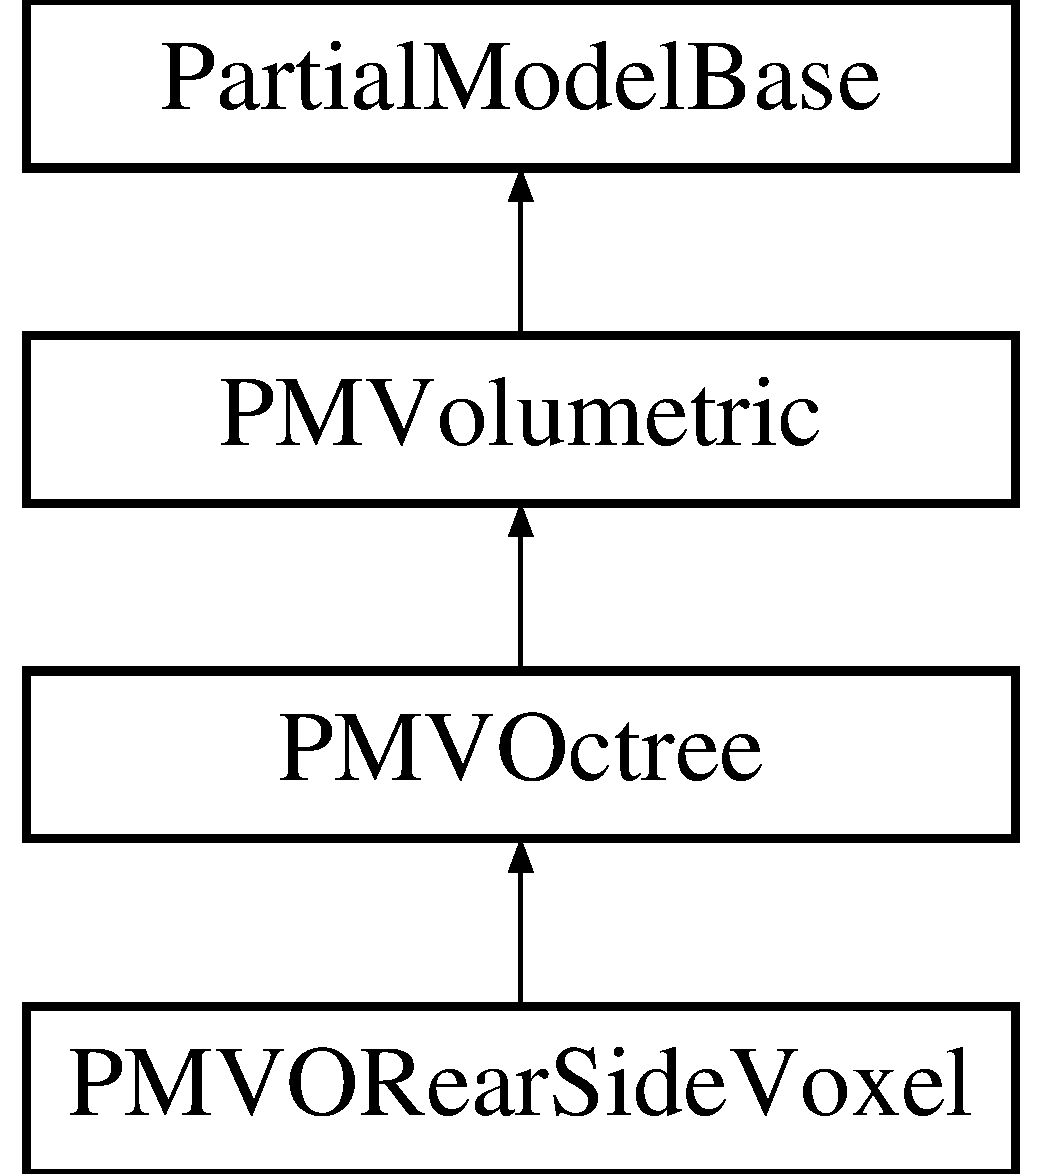
\includegraphics[height=4.000000cm]{classPMVORearSideVoxel}
\end{center}
\end{figure}
\subsection*{Public Member Functions}
\begin{DoxyCompactItemize}
\item 
virtual int \hyperlink{classPMVORearSideVoxel_abfbe9be1007d7d7fe7434031c1d96ad1}{evaluate\+View} (\hyperlink{classViewStructure}{View\+Structure} \&v)
\item 
virtual bool {\bfseries init} ()\hypertarget{classPMVORearSideVoxel_a4ca7c445000eca5a6adffb697144883f}{}\label{classPMVORearSideVoxel_a4ca7c445000eca5a6adffb697144883f}

\item 
virtual float {\bfseries update\+With\+Scan} (std\+::\+\_\+\+\_\+cxx11\+::string file\+\_\+name\+\_\+scan, std\+::\+\_\+\+\_\+cxx11\+::string file\+\_\+name\+\_\+origin)\hypertarget{classPMVORearSideVoxel_a38a6f20a57c209e87f74f5b4859271f7}{}\label{classPMVORearSideVoxel_a38a6f20a57c209e87f74f5b4859271f7}

\end{DoxyCompactItemize}
\subsection*{Protected Member Functions}
\begin{DoxyCompactItemize}
\item 
virtual bool \hyperlink{classPMVORearSideVoxel_afd9b08599913cf32cbc315cb210f4924}{ray\+Tracing\+H\+TM} (boost\+::numeric\+::ublas\+::matrix$<$ double $>$ m, \hyperlink{classEvaluationResult}{Evaluation\+Result} \&result)
\end{DoxyCompactItemize}
\subsection*{Additional Inherited Members}


\subsection{Member Function Documentation}
\index{P\+M\+V\+O\+Rear\+Side\+Voxel@{P\+M\+V\+O\+Rear\+Side\+Voxel}!evaluate\+View@{evaluate\+View}}
\index{evaluate\+View@{evaluate\+View}!P\+M\+V\+O\+Rear\+Side\+Voxel@{P\+M\+V\+O\+Rear\+Side\+Voxel}}
\subsubsection[{\texorpdfstring{evaluate\+View(\+View\+Structure \&v)}{evaluateView(ViewStructure &v)}}]{\setlength{\rightskip}{0pt plus 5cm}int P\+M\+V\+O\+Rear\+Side\+Voxel\+::evaluate\+View (
\begin{DoxyParamCaption}
\item[{{\bf View\+Structure} \&}]{v}
\end{DoxyParamCaption}
)\hspace{0.3cm}{\ttfamily [virtual]}}\hypertarget{classPMVORearSideVoxel_abfbe9be1007d7d7fe7434031c1d96ad1}{}\label{classPMVORearSideVoxel_abfbe9be1007d7d7fe7434031c1d96ad1}
Evaluate the result of the raytracing 

Reimplemented from \hyperlink{classPMVOctree_a2f35ea94079904f2e336776cec14b234}{P\+M\+V\+Octree}.

\index{P\+M\+V\+O\+Rear\+Side\+Voxel@{P\+M\+V\+O\+Rear\+Side\+Voxel}!ray\+Tracing\+H\+TM@{ray\+Tracing\+H\+TM}}
\index{ray\+Tracing\+H\+TM@{ray\+Tracing\+H\+TM}!P\+M\+V\+O\+Rear\+Side\+Voxel@{P\+M\+V\+O\+Rear\+Side\+Voxel}}
\subsubsection[{\texorpdfstring{ray\+Tracing\+H\+T\+M(boost\+::numeric\+::ublas\+::matrix$<$ double $>$ m, Evaluation\+Result \&result)}{rayTracingHTM(boost::numeric::ublas::matrix< double > m, EvaluationResult &result)}}]{\setlength{\rightskip}{0pt plus 5cm}bool P\+M\+V\+O\+Rear\+Side\+Voxel\+::ray\+Tracing\+H\+TM (
\begin{DoxyParamCaption}
\item[{boost\+::numeric\+::ublas\+::matrix$<$ double $>$}]{m, }
\item[{{\bf Evaluation\+Result} \&}]{result}
\end{DoxyParamCaption}
)\hspace{0.3cm}{\ttfamily [protected]}, {\ttfamily [virtual]}}\hypertarget{classPMVORearSideVoxel_afd9b08599913cf32cbc315cb210f4924}{}\label{classPMVORearSideVoxel_afd9b08599913cf32cbc315cb210f4924}
Gathers rearside voxels Rear\+Side voxels are returned in result.\+unknown voxels The ray is rotated and traslated by the rotation matrix 

Reimplemented from \hyperlink{classPMVOctree_a7f3ca384e40ac57446ec20d9acbefa92}{P\+M\+V\+Octree}.



The documentation for this class was generated from the following files\+:\begin{DoxyCompactItemize}
\item 
partialmodel/pmvorearsidevoxel.\+h\item 
partialmodel/pmvorearsidevoxel.\+cpp\end{DoxyCompactItemize}

\hypertarget{classR3DDirectPositioning}{}\section{R3\+D\+Direct\+Positioning Class Reference}
\label{classR3DDirectPositioning}\index{R3\+D\+Direct\+Positioning@{R3\+D\+Direct\+Positioning}}
Inheritance diagram for R3\+D\+Direct\+Positioning\+:\begin{figure}[H]
\begin{center}
\leavevmode
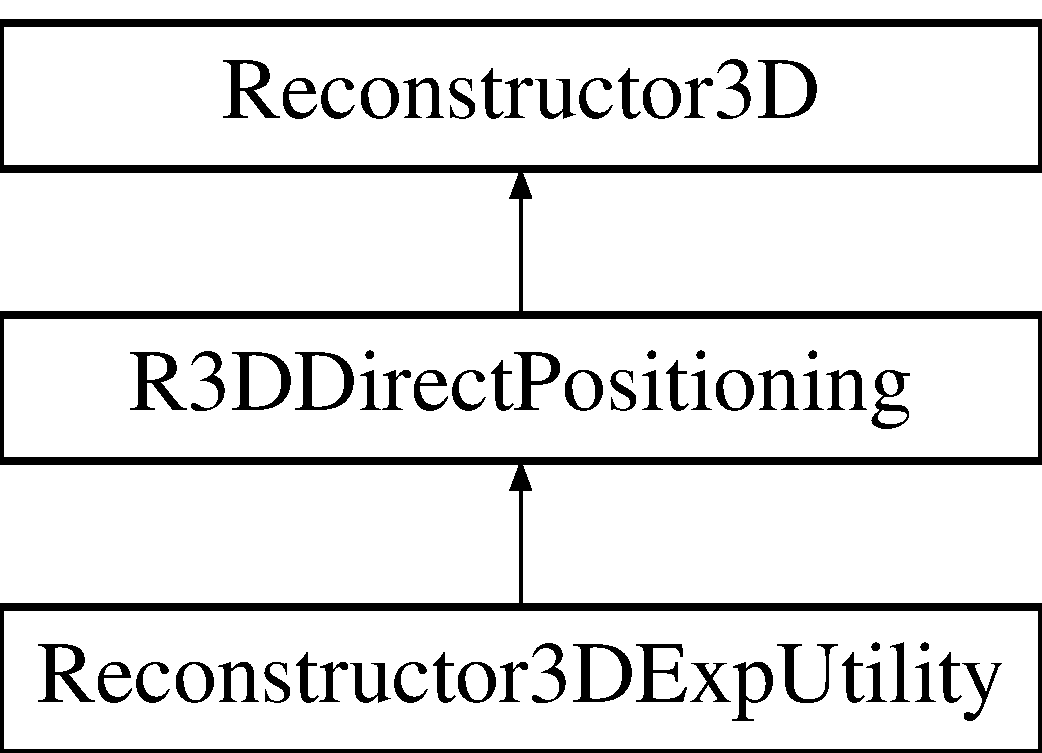
\includegraphics[height=3.000000cm]{classR3DDirectPositioning}
\end{center}
\end{figure}
\subsection*{Public Member Functions}
\begin{DoxyCompactItemize}
\item 
{\bfseries R3\+D\+Direct\+Positioning} (\hyperlink{classRobotSensor}{Robot\+Sensor} $\ast$rs, \hyperlink{classNBVPlanner}{N\+B\+V\+Planner} $\ast$p)\hypertarget{classR3DDirectPositioning_a9f070cad93a8f6e814e8cd9eea43dffb}{}\label{classR3DDirectPositioning_a9f070cad93a8f6e814e8cd9eea43dffb}

\item 
virtual bool {\bfseries positioning} (\hyperlink{classViewStructure}{View\+Structure} v)\hypertarget{classR3DDirectPositioning_ac0d2abf3990d2af285c0e608b55d2843}{}\label{classR3DDirectPositioning_ac0d2abf3990d2af285c0e608b55d2843}

\item 
virtual bool {\bfseries update\+Model} (std\+::string scan\+\_\+name, std\+::string origin\+\_\+name)\hypertarget{classR3DDirectPositioning_a09b8d4ae2f3a3d1360590dac43fcc72e}{}\label{classR3DDirectPositioning_a09b8d4ae2f3a3d1360590dac43fcc72e}

\item 
virtual bool \hyperlink{classR3DDirectPositioning_a8688c3962bf886cf99cd04ff0b0ee7a9}{init} ()
\end{DoxyCompactItemize}
\subsection*{Public Attributes}
\begin{DoxyCompactItemize}
\item 
std\+::string \hyperlink{classR3DDirectPositioning_a328fd507b2d871268e8d3534e0cc94af}{ref\+\_\+obj\+\_\+pts\+\_\+fn}
\item 
std\+::string \hyperlink{classR3DDirectPositioning_a156083c077bff5fa575d1f436108d85d}{tar\+\_\+pts\+\_\+fn}
\item 
std\+::string \hyperlink{classR3DDirectPositioning_a5b0188ce75a41eb131151b87d5838222}{reconstruction\+\_\+perc\+\_\+fn}
\item 
double \hyperlink{classR3DDirectPositioning_a1649f58b4c24dca72b16e8e76e53180a}{gap\+\_\+points}
\end{DoxyCompactItemize}
\subsection*{Additional Inherited Members}


\subsection{Member Function Documentation}
\index{R3\+D\+Direct\+Positioning@{R3\+D\+Direct\+Positioning}!init@{init}}
\index{init@{init}!R3\+D\+Direct\+Positioning@{R3\+D\+Direct\+Positioning}}
\subsubsection[{\texorpdfstring{init()}{init()}}]{\setlength{\rightskip}{0pt plus 5cm}bool R3\+D\+Direct\+Positioning\+::init (
\begin{DoxyParamCaption}
{}
\end{DoxyParamCaption}
)\hspace{0.3cm}{\ttfamily [virtual]}}\hypertarget{classR3DDirectPositioning_a8688c3962bf886cf99cd04ff0b0ee7a9}{}\label{classR3DDirectPositioning_a8688c3962bf886cf99cd04ff0b0ee7a9}
Initialices the N\+BV problem 

Reimplemented from \hyperlink{classReconstructor3D_a7ac7a63de2bfa609b1b0d15cde33f139}{Reconstructor3D}.



\subsection{Member Data Documentation}
\index{R3\+D\+Direct\+Positioning@{R3\+D\+Direct\+Positioning}!gap\+\_\+points@{gap\+\_\+points}}
\index{gap\+\_\+points@{gap\+\_\+points}!R3\+D\+Direct\+Positioning@{R3\+D\+Direct\+Positioning}}
\subsubsection[{\texorpdfstring{gap\+\_\+points}{gap_points}}]{\setlength{\rightskip}{0pt plus 5cm}double R3\+D\+Direct\+Positioning\+::gap\+\_\+points}\hypertarget{classR3DDirectPositioning_a1649f58b4c24dca72b16e8e76e53180a}{}\label{classR3DDirectPositioning_a1649f58b4c24dca72b16e8e76e53180a}
gap for determinig if two points match. Recosntruction percentage calculation \index{R3\+D\+Direct\+Positioning@{R3\+D\+Direct\+Positioning}!reconstruction\+\_\+perc\+\_\+fn@{reconstruction\+\_\+perc\+\_\+fn}}
\index{reconstruction\+\_\+perc\+\_\+fn@{reconstruction\+\_\+perc\+\_\+fn}!R3\+D\+Direct\+Positioning@{R3\+D\+Direct\+Positioning}}
\subsubsection[{\texorpdfstring{reconstruction\+\_\+perc\+\_\+fn}{reconstruction_perc_fn}}]{\setlength{\rightskip}{0pt plus 5cm}std\+::string R3\+D\+Direct\+Positioning\+::reconstruction\+\_\+perc\+\_\+fn}\hypertarget{classR3DDirectPositioning_a5b0188ce75a41eb131151b87d5838222}{}\label{classR3DDirectPositioning_a5b0188ce75a41eb131151b87d5838222}
Reconstruction percentage filename \index{R3\+D\+Direct\+Positioning@{R3\+D\+Direct\+Positioning}!ref\+\_\+obj\+\_\+pts\+\_\+fn@{ref\+\_\+obj\+\_\+pts\+\_\+fn}}
\index{ref\+\_\+obj\+\_\+pts\+\_\+fn@{ref\+\_\+obj\+\_\+pts\+\_\+fn}!R3\+D\+Direct\+Positioning@{R3\+D\+Direct\+Positioning}}
\subsubsection[{\texorpdfstring{ref\+\_\+obj\+\_\+pts\+\_\+fn}{ref_obj_pts_fn}}]{\setlength{\rightskip}{0pt plus 5cm}std\+::string R3\+D\+Direct\+Positioning\+::ref\+\_\+obj\+\_\+pts\+\_\+fn}\hypertarget{classR3DDirectPositioning_a328fd507b2d871268e8d3534e0cc94af}{}\label{classR3DDirectPositioning_a328fd507b2d871268e8d3534e0cc94af}
Reference object points filename. The points are used to compare the percentage of reconstruction \index{R3\+D\+Direct\+Positioning@{R3\+D\+Direct\+Positioning}!tar\+\_\+pts\+\_\+fn@{tar\+\_\+pts\+\_\+fn}}
\index{tar\+\_\+pts\+\_\+fn@{tar\+\_\+pts\+\_\+fn}!R3\+D\+Direct\+Positioning@{R3\+D\+Direct\+Positioning}}
\subsubsection[{\texorpdfstring{tar\+\_\+pts\+\_\+fn}{tar_pts_fn}}]{\setlength{\rightskip}{0pt plus 5cm}std\+::string R3\+D\+Direct\+Positioning\+::tar\+\_\+pts\+\_\+fn}\hypertarget{classR3DDirectPositioning_a156083c077bff5fa575d1f436108d85d}{}\label{classR3DDirectPositioning_a156083c077bff5fa575d1f436108d85d}
Target points filename (Accumulated points from the reconstruction). The points are used to compare the percentage of reconstruction 

The documentation for this class was generated from the following files\+:\begin{DoxyCompactItemize}
\item 
viewplanning/r3ddirectpositioning.\+h\item 
viewplanning/r3ddirectpositioning.\+cpp\end{DoxyCompactItemize}

\hypertarget{classRandomViewSynthesis}{}\section{Random\+View\+Synthesis Class Reference}
\label{classRandomViewSynthesis}\index{Random\+View\+Synthesis@{Random\+View\+Synthesis}}
Inheritance diagram for Random\+View\+Synthesis\+:\begin{figure}[H]
\begin{center}
\leavevmode
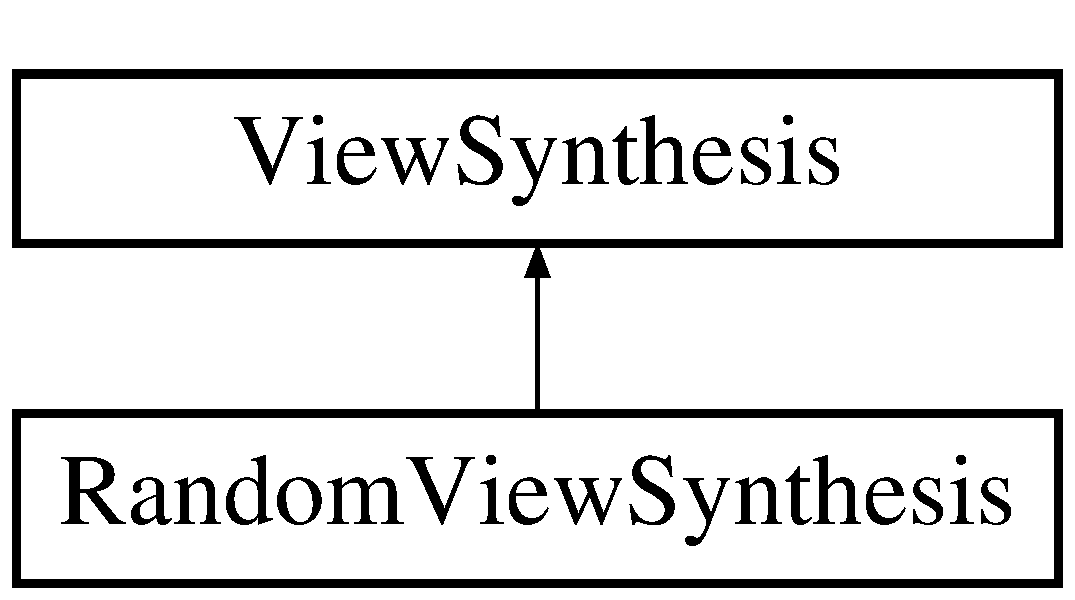
\includegraphics[height=2.000000cm]{classRandomViewSynthesis}
\end{center}
\end{figure}
\subsection*{Public Member Functions}
\begin{DoxyCompactItemize}
\item 
{\bfseries Random\+View\+Synthesis} (int n, \hyperlink{classViewStructure}{View\+Structure} min, \hyperlink{classViewStructure}{View\+Structure} max)\hypertarget{classRandomViewSynthesis_a1a7d2d9d1f1163e982ca6ea924e37abe}{}\label{classRandomViewSynthesis_a1a7d2d9d1f1163e982ca6ea924e37abe}

\item 
virtual void {\bfseries get\+Views} (\hyperlink{classViewList}{View\+List} \&views)\hypertarget{classRandomViewSynthesis_a1d994dab6b363f2b0a933d4db3b72cae}{}\label{classRandomViewSynthesis_a1d994dab6b363f2b0a933d4db3b72cae}

\end{DoxyCompactItemize}
\subsection*{Protected Attributes}
\begin{DoxyCompactItemize}
\item 
\hyperlink{classViewStructure}{View\+Structure} {\bfseries min\+\_\+view}\hypertarget{classRandomViewSynthesis_a558492e6e61291f879734a76aeabaf87}{}\label{classRandomViewSynthesis_a558492e6e61291f879734a76aeabaf87}

\item 
\hyperlink{classViewStructure}{View\+Structure} {\bfseries max\+\_\+view}\hypertarget{classRandomViewSynthesis_a98229413d688af47c3747becd708d949}{}\label{classRandomViewSynthesis_a98229413d688af47c3747becd708d949}

\end{DoxyCompactItemize}


The documentation for this class was generated from the following files\+:\begin{DoxyCompactItemize}
\item 
partialmodel/viewsynthesis.\+h\item 
partialmodel/viewsynthesis.\+cpp\end{DoxyCompactItemize}

\hypertarget{classRangeSensor}{}\section{Range\+Sensor Class Reference}
\label{classRangeSensor}\index{Range\+Sensor@{Range\+Sensor}}


{\ttfamily \#include $<$rangesensor.\+h$>$}

\subsection*{Public Member Functions}
\begin{DoxyCompactItemize}
\item 
virtual bool {\bfseries init} ()\hypertarget{classRangeSensor_a0fa9437a62cec4c93ea3f74472d67d3c}{}\label{classRangeSensor_a0fa9437a62cec4c93ea3f74472d67d3c}

\item 
virtual long int \hyperlink{classRangeSensor_a41e0ee652ab717ed803271f944f229d2}{get\+Points} (std\+::vector$<$ mrpt\+::poses\+::\+C\+Point3D $>$ \&points)=0
\item 
virtual void \hyperlink{classRangeSensor_a3c66f28c18e3fe8ffba809a8d9d83f62}{get\+Rays} (std\+::vector$<$ std\+::vector$<$ double $>$ $>$ \&rays)
\item 
bool {\bfseries save\+Rays} (std\+::string filename)\hypertarget{classRangeSensor_a0bdf89af52158d28f030523254509dbe}{}\label{classRangeSensor_a0bdf89af52158d28f030523254509dbe}

\item 
virtual long int \hyperlink{classRangeSensor_a29bca03aff4a2392ab34ded51d74ab92}{get\+Rays\+For\+Resolution} (std\+::vector$<$ std\+::vector$<$ double $>$ $>$ \&rays, double resolution, double distance)
\item 
bool \hyperlink{classRangeSensor_a9d8589690833d9294092449b8daf5ce7}{save\+Rays\+For\+Resolution} (std\+::string filename, double resolution, double distance)
\item 
void \hyperlink{classRangeSensor_afdccf7af7a35e9d83fbb5f0dbab1019d}{get\+Info} (std\+::string \&txt)
\item 
void {\bfseries set\+Config\+Folder} (std\+::string folder)\hypertarget{classRangeSensor_a61c318a0c38450e8c89b0aeeccee350d}{}\label{classRangeSensor_a61c318a0c38450e8c89b0aeeccee350d}

\item 
void {\bfseries set\+Data\+Folder} (std\+::string folder)\hypertarget{classRangeSensor_a116cb7188af13268484e4f7aee1d33de}{}\label{classRangeSensor_a116cb7188af13268484e4f7aee1d33de}

\item 
void {\bfseries get\+Director\+Ray} (std\+::vector$<$ double $>$ \&ray)\hypertarget{classRangeSensor_adfba7fd830d21af871359b959d1ac44d}{}\label{classRangeSensor_adfba7fd830d21af871359b959d1ac44d}

\item 
void {\bfseries set\+Current\+View} (\hyperlink{classViewStructure}{View\+Structure} v)\hypertarget{classRangeSensor_a4955219c175c9ba2da8a0cb743bb703f}{}\label{classRangeSensor_a4955219c175c9ba2da8a0cb743bb703f}

\end{DoxyCompactItemize}
\subsection*{Protected Attributes}
\begin{DoxyCompactItemize}
\item 
double {\bfseries h\+\_\+aperture}\hypertarget{classRangeSensor_a333835abaf69fe389a6c4003a05025e9}{}\label{classRangeSensor_a333835abaf69fe389a6c4003a05025e9}

\item 
double {\bfseries v\+\_\+aperture}\hypertarget{classRangeSensor_a8a611c5adff94034e5d057cbfbd9b06e}{}\label{classRangeSensor_a8a611c5adff94034e5d057cbfbd9b06e}

\item 
int {\bfseries h\+\_\+points}\hypertarget{classRangeSensor_aa4bd70ed9a9ed097b0f1e0a1b63f7710}{}\label{classRangeSensor_aa4bd70ed9a9ed097b0f1e0a1b63f7710}

\item 
int {\bfseries v\+\_\+points}\hypertarget{classRangeSensor_ae41a872ce9c80fe142e03a245dd7e11b}{}\label{classRangeSensor_ae41a872ce9c80fe142e03a245dd7e11b}

\item 
std\+::string {\bfseries info}\hypertarget{classRangeSensor_a48ddb91baf886a7f69a23be2e24961d8}{}\label{classRangeSensor_a48ddb91baf886a7f69a23be2e24961d8}

\item 
bool {\bfseries ready}\hypertarget{classRangeSensor_a39b6258b5c2ea3cc92f64e85f2731fab}{}\label{classRangeSensor_a39b6258b5c2ea3cc92f64e85f2731fab}

\item 
std\+::string {\bfseries config\+Folder}\hypertarget{classRangeSensor_af275904c340a557cf90e623468deea8e}{}\label{classRangeSensor_af275904c340a557cf90e623468deea8e}

\item 
std\+::string {\bfseries data\+Folder}\hypertarget{classRangeSensor_a1c28d60485ff932cb00b838c27761918}{}\label{classRangeSensor_a1c28d60485ff932cb00b838c27761918}

\item 
std\+::vector$<$ double $>$ {\bfseries director\+\_\+ray}\hypertarget{classRangeSensor_a0a58e87804d43700b307eb7346be352c}{}\label{classRangeSensor_a0a58e87804d43700b307eb7346be352c}

\item 
\hyperlink{classViewStructure}{View\+Structure} \hyperlink{classRangeSensor_a35c0f1409284433393081ff9b048766d}{current\+View}\hypertarget{classRangeSensor_a35c0f1409284433393081ff9b048766d}{}\label{classRangeSensor_a35c0f1409284433393081ff9b048766d}

\begin{DoxyCompactList}\small\item\em Only required for simulated sensors. \end{DoxyCompactList}\end{DoxyCompactItemize}


\subsection{Detailed Description}
Defines a Range Sensor. It abstracs the communication with the device. Returns a set of poins in the 3D space as a read. All units must be in mts and rads; 

\subsection{Member Function Documentation}
\index{Range\+Sensor@{Range\+Sensor}!get\+Info@{get\+Info}}
\index{get\+Info@{get\+Info}!Range\+Sensor@{Range\+Sensor}}
\subsubsection[{\texorpdfstring{get\+Info(std\+::string \&txt)}{getInfo(std::string &txt)}}]{\setlength{\rightskip}{0pt plus 5cm}void Range\+Sensor\+::get\+Info (
\begin{DoxyParamCaption}
\item[{std\+::string \&}]{txt}
\end{DoxyParamCaption}
)}\hypertarget{classRangeSensor_afdccf7af7a35e9d83fbb5f0dbab1019d}{}\label{classRangeSensor_afdccf7af7a35e9d83fbb5f0dbab1019d}
Returns information about the sensor \index{Range\+Sensor@{Range\+Sensor}!get\+Points@{get\+Points}}
\index{get\+Points@{get\+Points}!Range\+Sensor@{Range\+Sensor}}
\subsubsection[{\texorpdfstring{get\+Points(std\+::vector$<$ mrpt\+::poses\+::\+C\+Point3\+D $>$ \&points)=0}{getPoints(std::vector< mrpt::poses::CPoint3D > &points)=0}}]{\setlength{\rightskip}{0pt plus 5cm}virtual long int Range\+Sensor\+::get\+Points (
\begin{DoxyParamCaption}
\item[{std\+::vector$<$ mrpt\+::poses\+::\+C\+Point3D $>$ \&}]{points}
\end{DoxyParamCaption}
)\hspace{0.3cm}{\ttfamily [pure virtual]}}\hypertarget{classRangeSensor_a41e0ee652ab717ed803271f944f229d2}{}\label{classRangeSensor_a41e0ee652ab717ed803271f944f229d2}
Reads the sensor and get 3D points in mm \index{Range\+Sensor@{Range\+Sensor}!get\+Rays@{get\+Rays}}
\index{get\+Rays@{get\+Rays}!Range\+Sensor@{Range\+Sensor}}
\subsubsection[{\texorpdfstring{get\+Rays(std\+::vector$<$ std\+::vector$<$ double $>$ $>$ \&rays)}{getRays(std::vector< std::vector< double > > &rays)}}]{\setlength{\rightskip}{0pt plus 5cm}void Range\+Sensor\+::get\+Rays (
\begin{DoxyParamCaption}
\item[{std\+::vector$<$ std\+::vector$<$ double $>$ $>$ \&}]{rays}
\end{DoxyParamCaption}
)\hspace{0.3cm}{\ttfamily [virtual]}}\hypertarget{classRangeSensor_a3c66f28c18e3fe8ffba809a8d9d83f62}{}\label{classRangeSensor_a3c66f28c18e3fe8ffba809a8d9d83f62}
Returns the set of rays which define the sensor \index{Range\+Sensor@{Range\+Sensor}!get\+Rays\+For\+Resolution@{get\+Rays\+For\+Resolution}}
\index{get\+Rays\+For\+Resolution@{get\+Rays\+For\+Resolution}!Range\+Sensor@{Range\+Sensor}}
\subsubsection[{\texorpdfstring{get\+Rays\+For\+Resolution(std\+::vector$<$ std\+::vector$<$ double $>$ $>$ \&rays, double resolution, double distance)}{getRaysForResolution(std::vector< std::vector< double > > &rays, double resolution, double distance)}}]{\setlength{\rightskip}{0pt plus 5cm}long int Range\+Sensor\+::get\+Rays\+For\+Resolution (
\begin{DoxyParamCaption}
\item[{std\+::vector$<$ std\+::vector$<$ double $>$ $>$ \&}]{rays, }
\item[{double}]{resolution, }
\item[{double}]{distance}
\end{DoxyParamCaption}
)\hspace{0.3cm}{\ttfamily [virtual]}}\hypertarget{classRangeSensor_a29bca03aff4a2392ab34ded51d74ab92}{}\label{classRangeSensor_a29bca03aff4a2392ab34ded51d74ab92}
Computes a set of minimun rays for the voxel resolution especified resolution must have the same units than distance \index{Range\+Sensor@{Range\+Sensor}!save\+Rays\+For\+Resolution@{save\+Rays\+For\+Resolution}}
\index{save\+Rays\+For\+Resolution@{save\+Rays\+For\+Resolution}!Range\+Sensor@{Range\+Sensor}}
\subsubsection[{\texorpdfstring{save\+Rays\+For\+Resolution(std\+::string filename, double resolution, double distance)}{saveRaysForResolution(std::string filename, double resolution, double distance)}}]{\setlength{\rightskip}{0pt plus 5cm}bool Range\+Sensor\+::save\+Rays\+For\+Resolution (
\begin{DoxyParamCaption}
\item[{std\+::string}]{filename, }
\item[{double}]{resolution, }
\item[{double}]{distance}
\end{DoxyParamCaption}
)}\hypertarget{classRangeSensor_a9d8589690833d9294092449b8daf5ce7}{}\label{classRangeSensor_a9d8589690833d9294092449b8daf5ce7}
Saves a \char`\"{}ideal\char`\"{} subset of rays depending on the resolution of the octree and the distance from the sensor resolution must have the same units than distance 

The documentation for this class was generated from the following files\+:\begin{DoxyCompactItemize}
\item 
viewplanning/rangesensor.\+h\item 
viewplanning/rangesensor.\+cpp\end{DoxyCompactItemize}

\hypertarget{classReconstructor3D}{}\section{Reconstructor3D Class Reference}
\label{classReconstructor3D}\index{Reconstructor3D@{Reconstructor3D}}


{\ttfamily \#include $<$reconstructor3d.\+h$>$}

Inheritance diagram for Reconstructor3D\+:\begin{figure}[H]
\begin{center}
\leavevmode
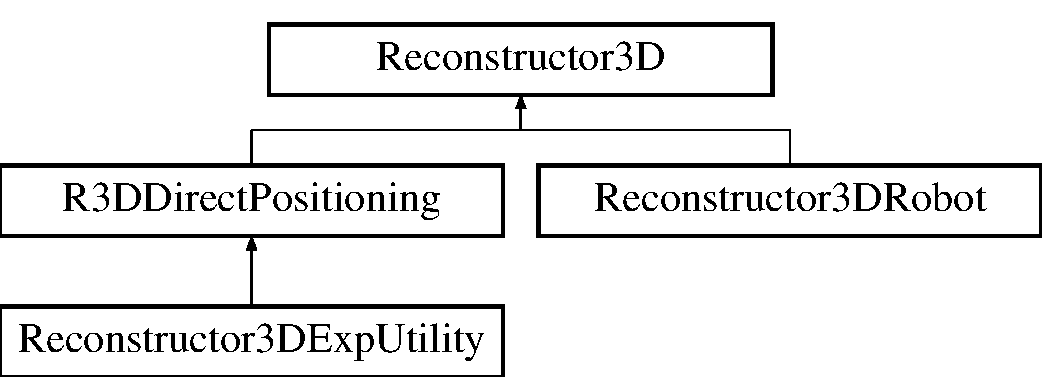
\includegraphics[height=3.000000cm]{classReconstructor3D}
\end{center}
\end{figure}
\subsection*{Public Member Functions}
\begin{DoxyCompactItemize}
\item 
{\bfseries Reconstructor3D} (\hyperlink{classRobotSensor}{Robot\+Sensor} $\ast$rs, \hyperlink{classNBVPlanner}{N\+B\+V\+Planner} $\ast$p)\hypertarget{classReconstructor3D_a6dc91fcadae64d16bf72d98072e109dc}{}\label{classReconstructor3D_a6dc91fcadae64d16bf72d98072e109dc}

\item 
virtual bool \hyperlink{classReconstructor3D_a7ac7a63de2bfa609b1b0d15cde33f139}{init} ()
\item 
virtual bool {\bfseries positioning} (\hyperlink{classViewStructure}{View\+Structure} v)=0\hypertarget{classReconstructor3D_a00be85ea925b48d3e5ec1e773a9c5846}{}\label{classReconstructor3D_a00be85ea925b48d3e5ec1e773a9c5846}

\item 
virtual void {\bfseries save\+Data} ()\hypertarget{classReconstructor3D_a2368a98c5421e08f91881cf2faa8689a}{}\label{classReconstructor3D_a2368a98c5421e08f91881cf2faa8689a}

\item 
virtual bool \hyperlink{classReconstructor3D_ac4433ce176af00bd57a79d67d0fc4a14}{take\+Scan} (std\+::string \&scan\+\_\+name, std\+::string \&origin\+\_\+name)
\item 
virtual \hyperlink{classViewStructure}{View\+Structure} {\bfseries Plan\+Next\+Best\+View} ()\hypertarget{classReconstructor3D_a70ee2a6553cc0e92e15bbf55574aa9f5}{}\label{classReconstructor3D_a70ee2a6553cc0e92e15bbf55574aa9f5}

\item 
virtual bool {\bfseries update\+Model} (std\+::string scan\+\_\+name, std\+::string origin\+\_\+name)\hypertarget{classReconstructor3D_a10279e3dd4100d1a9c334c38e2ed01c9}{}\label{classReconstructor3D_a10279e3dd4100d1a9c334c38e2ed01c9}

\item 
virtual bool {\bfseries stop\+Criteria\+Satisfied} ()\hypertarget{classReconstructor3D_aadea36c1a4989198e092b60a299f8729}{}\label{classReconstructor3D_aadea36c1a4989198e092b60a299f8729}

\item 
virtual void {\bfseries finish\+Reconstruction} ()\hypertarget{classReconstructor3D_a77464b426265ab191b87e32b0160ac52}{}\label{classReconstructor3D_a77464b426265ab191b87e32b0160ac52}

\item 
void {\bfseries solve\+Reconstruction} ()\hypertarget{classReconstructor3D_ab45520b4bd55fbd6fc222aae759b8f0c}{}\label{classReconstructor3D_ab45520b4bd55fbd6fc222aae759b8f0c}

\item 
void {\bfseries set\+N\+Generated\+Views} (int n)\hypertarget{classReconstructor3D_a56b79062b049931f767f2d6451bfab3b}{}\label{classReconstructor3D_a56b79062b049931f767f2d6451bfab3b}

\item 
void {\bfseries set\+Data\+Folder} (std\+::string folder)\hypertarget{classReconstructor3D_a5cc843ea32ec0152a059318c47728d12}{}\label{classReconstructor3D_a5cc843ea32ec0152a059318c47728d12}

\item 
void {\bfseries set\+Config\+Folder} (std\+::string folder)\hypertarget{classReconstructor3D_ad41a7a58bff926bb2162ae55f850e011}{}\label{classReconstructor3D_ad41a7a58bff926bb2162ae55f850e011}

\item 
bool {\bfseries start\+Log\+File} ()\hypertarget{classReconstructor3D_a3d69e32e5f51b48437220ce61390a993}{}\label{classReconstructor3D_a3d69e32e5f51b48437220ce61390a993}

\item 
bool {\bfseries save\+To\+Log\+File} ()\hypertarget{classReconstructor3D_a3919d24a3df7aa41da8b0d273c50b1db}{}\label{classReconstructor3D_a3919d24a3df7aa41da8b0d273c50b1db}

\item 
void {\bfseries set\+Partial\+Model} (\hyperlink{classPartialModelBase}{Partial\+Model\+Base} $\ast$pm)\hypertarget{classReconstructor3D_a35c956aaa1e0a4af2bcd0d91e7406cd1}{}\label{classReconstructor3D_a35c956aaa1e0a4af2bcd0d91e7406cd1}

\end{DoxyCompactItemize}
\subsection*{Protected Attributes}
\begin{DoxyCompactItemize}
\item 
bool {\bfseries wait\+For\+User}\hypertarget{classReconstructor3D_a116e39fd7cf2c85d84f4d90726caa439}{}\label{classReconstructor3D_a116e39fd7cf2c85d84f4d90726caa439}

\item 
bool {\bfseries update\+Robot\+Localization}\hypertarget{classReconstructor3D_a1d13f9650030fe143c07bad08d7ec122}{}\label{classReconstructor3D_a1d13f9650030fe143c07bad08d7ec122}

\item 
int {\bfseries max\+Iterations}\hypertarget{classReconstructor3D_aaac001d16a46512928f90fdfa8e3ab31}{}\label{classReconstructor3D_aaac001d16a46512928f90fdfa8e3ab31}

\item 
\hyperlink{classPartialModelBase}{Partial\+Model\+Base} $\ast$ {\bfseries partial\+Model}\hypertarget{classReconstructor3D_a9d6e0bcc66b57b9854bf88fa193dd53f}{}\label{classReconstructor3D_a9d6e0bcc66b57b9854bf88fa193dd53f}

\item 
\hyperlink{classRobotSensor}{Robot\+Sensor} $\ast$ {\bfseries robot\+\_\+sensor}\hypertarget{classReconstructor3D_a04e0b53c72fb1ca3f3442d201dafe93d}{}\label{classReconstructor3D_a04e0b53c72fb1ca3f3442d201dafe93d}

\item 
\hyperlink{classNBVPlanner}{N\+B\+V\+Planner} $\ast$ {\bfseries planner}\hypertarget{classReconstructor3D_af4850cdebe3a45a5f0b10502d15f49f4}{}\label{classReconstructor3D_af4850cdebe3a45a5f0b10502d15f49f4}

\item 
std\+::string {\bfseries data\+Folder}\hypertarget{classReconstructor3D_a9dda51c8d96892f960a2156b9ebbf459}{}\label{classReconstructor3D_a9dda51c8d96892f960a2156b9ebbf459}

\item 
std\+::string {\bfseries config\+Folder}\hypertarget{classReconstructor3D_a5c130ef5c7fbb62a895211c01581065e}{}\label{classReconstructor3D_a5c130ef5c7fbb62a895211c01581065e}

\item 
std\+::string {\bfseries scan\+File\+Name}\hypertarget{classReconstructor3D_a121ef8abf670ad841e595679b4aecf0b}{}\label{classReconstructor3D_a121ef8abf670ad841e595679b4aecf0b}

\item 
std\+::string {\bfseries origin\+File\+Name}\hypertarget{classReconstructor3D_a89792f8628eda6c46cefc55c378a1357}{}\label{classReconstructor3D_a89792f8628eda6c46cefc55c378a1357}

\item 
std\+::string {\bfseries candidate\+Views\+File\+Name}\hypertarget{classReconstructor3D_aa0c2389c278bd55458ee2987f934f158}{}\label{classReconstructor3D_aa0c2389c278bd55458ee2987f934f158}

\item 
std\+::string {\bfseries rays\+File\+Name}\hypertarget{classReconstructor3D_a683bf47fbcf5e02cafaa6ed64e5c8808}{}\label{classReconstructor3D_a683bf47fbcf5e02cafaa6ed64e5c8808}

\item 
std\+::string {\bfseries goals\+File\+Name}\hypertarget{classReconstructor3D_a9d8445fd97ce76f197a83201dacb0b3b}{}\label{classReconstructor3D_a9d8445fd97ce76f197a83201dacb0b3b}

\item 
std\+::string {\bfseries reached\+Goals\+Filename}\hypertarget{classReconstructor3D_a74620d1907a23d43e11ca38f4ed2c035}{}\label{classReconstructor3D_a74620d1907a23d43e11ca38f4ed2c035}

\item 
std\+::string {\bfseries partial\+Model\+File\+Name}\hypertarget{classReconstructor3D_a986fa32b1e25e94f53f6e72395da67b8}{}\label{classReconstructor3D_a986fa32b1e25e94f53f6e72395da67b8}

\item 
std\+::string {\bfseries occupied\+Voxels\+File\+Name}\hypertarget{classReconstructor3D_a063c1b092b9d852d652b01f9c8d1b746}{}\label{classReconstructor3D_a063c1b092b9d852d652b01f9c8d1b746}

\item 
std\+::string {\bfseries unknown\+Voxels\+Filename}\hypertarget{classReconstructor3D_a175169ef3cfc0ae3e093f1c3a8878746}{}\label{classReconstructor3D_a175169ef3cfc0ae3e093f1c3a8878746}

\item 
std\+::string {\bfseries current\+Point\+Cloud\+File}\hypertarget{classReconstructor3D_a141c9795c4112380913575958f88c342}{}\label{classReconstructor3D_a141c9795c4112380913575958f88c342}

\item 
std\+::string {\bfseries current\+Origin\+File}\hypertarget{classReconstructor3D_ab93757b22b3da8436dd133d49d647ff9}{}\label{classReconstructor3D_ab93757b22b3da8436dd133d49d647ff9}

\item 
long int {\bfseries n\+\_\+views}\hypertarget{classReconstructor3D_af7694b142f1ee0188b1c210f5ad91771}{}\label{classReconstructor3D_af7694b142f1ee0188b1c210f5ad91771}

\item 
int {\bfseries iteration}\hypertarget{classReconstructor3D_ad6b3d3579381d6b919d3480dc544aa68}{}\label{classReconstructor3D_ad6b3d3579381d6b919d3480dc544aa68}

\item 
std\+::vector$<$ std\+::vector$<$ int $>$ $>$ \hyperlink{classReconstructor3D_aecbe4257f53cc243125a8c370265e8de}{configs}\hypertarget{classReconstructor3D_aecbe4257f53cc243125a8c370265e8de}{}\label{classReconstructor3D_aecbe4257f53cc243125a8c370265e8de}

\begin{DoxyCompactList}\small\item\em config to reach N\+BV \end{DoxyCompactList}\item 
int {\bfseries n\+\_\+subset\+\_\+to\+\_\+motion}\hypertarget{classReconstructor3D_af15e3bc3feca4c1cf3c1db6c275ab2b8}{}\label{classReconstructor3D_af15e3bc3feca4c1cf3c1db6c275ab2b8}

\item 
std\+::list$<$ \hyperlink{classViewStructure}{View\+Structure} $>$ \hyperlink{classReconstructor3D_a8afd09b3f07435ef93b11147b0d92c6f}{Plan}
\item 
\hyperlink{classViewStructure}{View\+Structure} \hyperlink{classReconstructor3D_a29b49aed1badf557f570f835d8683532}{current\+View}
\item 
bool {\bfseries initiated}\hypertarget{classReconstructor3D_a2e701750963834a8452e3a7bd75a09c0}{}\label{classReconstructor3D_a2e701750963834a8452e3a7bd75a09c0}

\item 
float \hyperlink{classReconstructor3D_a430c767504d2bdcd445929456889f8e9}{std\+\_\+utility}\hypertarget{classReconstructor3D_a430c767504d2bdcd445929456889f8e9}{}\label{classReconstructor3D_a430c767504d2bdcd445929456889f8e9}

\begin{DoxyCompactList}\small\item\em stadistical variables \end{DoxyCompactList}\item 
float {\bfseries std\+\_\+surface\+\_\+utility}\hypertarget{classReconstructor3D_a460a06b85c058fbe3b385bfc08343764}{}\label{classReconstructor3D_a460a06b85c058fbe3b385bfc08343764}

\item 
float {\bfseries std\+\_\+distance\+\_\+utility}\hypertarget{classReconstructor3D_a5cbb62afa7c49ddf3df42d095e7fdbe3}{}\label{classReconstructor3D_a5cbb62afa7c49ddf3df42d095e7fdbe3}

\item 
float {\bfseries std\+\_\+unk\+\_\+voxel}\hypertarget{classReconstructor3D_ada173c8ac6804eb9f6d1173bd5c8bd63}{}\label{classReconstructor3D_ada173c8ac6804eb9f6d1173bd5c8bd63}

\item 
float {\bfseries std\+\_\+occ\+\_\+voxel}\hypertarget{classReconstructor3D_a4a93510c0ba7633a72982362712bdf72}{}\label{classReconstructor3D_a4a93510c0ba7633a72982362712bdf72}

\item 
float {\bfseries std\+\_\+reconstruction\+\_\+percent}\hypertarget{classReconstructor3D_a66fa77805a125d4cb469965f4fa56c21}{}\label{classReconstructor3D_a66fa77805a125d4cb469965f4fa56c21}

\item 
float {\bfseries std\+\_\+dist}\hypertarget{classReconstructor3D_a62aed9bb1f6ec8d83cd10c5f849779f0}{}\label{classReconstructor3D_a62aed9bb1f6ec8d83cd10c5f849779f0}

\item 
float {\bfseries std\+\_\+accumulated\+\_\+dist}\hypertarget{classReconstructor3D_ae8820c4efbb66caeeea375f7769d9a02}{}\label{classReconstructor3D_ae8820c4efbb66caeeea375f7769d9a02}

\item 
float {\bfseries std\+\_\+update\+\_\+t}\hypertarget{classReconstructor3D_a516eb9e47ad5b4e89204454fd10bad24}{}\label{classReconstructor3D_a516eb9e47ad5b4e89204454fd10bad24}

\item 
float {\bfseries std\+\_\+registration\+\_\+t}\hypertarget{classReconstructor3D_adf488d60da9bfb679f4c3344ff584453}{}\label{classReconstructor3D_adf488d60da9bfb679f4c3344ff584453}

\item 
float {\bfseries std\+\_\+vision\+\_\+t}\hypertarget{classReconstructor3D_a167bf09ad9ab88a7db23f8ef7c14a464}{}\label{classReconstructor3D_a167bf09ad9ab88a7db23f8ef7c14a464}

\item 
float {\bfseries std\+\_\+motionplanning\+\_\+t}\hypertarget{classReconstructor3D_a85b3a120dd77a0305d9d4c97b7da4dc8}{}\label{classReconstructor3D_a85b3a120dd77a0305d9d4c97b7da4dc8}

\item 
float {\bfseries std\+\_\+positioning\+\_\+t}\hypertarget{classReconstructor3D_af6bf8a303a6f2b4f39be4739d745e131}{}\label{classReconstructor3D_af6bf8a303a6f2b4f39be4739d745e131}

\item 
float {\bfseries std\+\_\+total\+\_\+time}\hypertarget{classReconstructor3D_a9fe8bb2f80c8b4cf04dfc7037410d1fa}{}\label{classReconstructor3D_a9fe8bb2f80c8b4cf04dfc7037410d1fa}

\item 
double {\bfseries std\+\_\+unknown\+\_\+volume}\hypertarget{classReconstructor3D_a2e6015d02aea82eeea87ead03422a5f7}{}\label{classReconstructor3D_a2e6015d02aea82eeea87ead03422a5f7}

\item 
float {\bfseries std\+\_\+probability}\hypertarget{classReconstructor3D_a1b3c8533b14c30586b326bacc7f79439}{}\label{classReconstructor3D_a1b3c8533b14c30586b326bacc7f79439}

\end{DoxyCompactItemize}


\subsection{Detailed Description}
Solves a Reconstruction Problem At the indicated directory must be the following files\+: -\/p0.\+vs Initial view in \hyperlink{classViewStructure}{View\+Structure} Format 

\subsection{Member Function Documentation}
\index{Reconstructor3D@{Reconstructor3D}!init@{init}}
\index{init@{init}!Reconstructor3D@{Reconstructor3D}}
\subsubsection[{\texorpdfstring{init()}{init()}}]{\setlength{\rightskip}{0pt plus 5cm}bool Reconstructor3\+D\+::init (
\begin{DoxyParamCaption}
{}
\end{DoxyParamCaption}
)\hspace{0.3cm}{\ttfamily [virtual]}}\hypertarget{classReconstructor3D_a7ac7a63de2bfa609b1b0d15cde33f139}{}\label{classReconstructor3D_a7ac7a63de2bfa609b1b0d15cde33f139}
Initialices the N\+BV problem 

Reimplemented in \hyperlink{classR3DDirectPositioning_a8688c3962bf886cf99cd04ff0b0ee7a9}{R3\+D\+Direct\+Positioning}.

\index{Reconstructor3D@{Reconstructor3D}!take\+Scan@{take\+Scan}}
\index{take\+Scan@{take\+Scan}!Reconstructor3D@{Reconstructor3D}}
\subsubsection[{\texorpdfstring{take\+Scan(std\+::string \&scan\+\_\+name, std\+::string \&origin\+\_\+name)}{takeScan(std::string &scan_name, std::string &origin_name)}}]{\setlength{\rightskip}{0pt plus 5cm}bool Reconstructor3\+D\+::take\+Scan (
\begin{DoxyParamCaption}
\item[{std\+::string \&}]{scan\+\_\+name, }
\item[{std\+::string \&}]{origin\+\_\+name}
\end{DoxyParamCaption}
)\hspace{0.3cm}{\ttfamily [virtual]}}\hypertarget{classReconstructor3D_ac4433ce176af00bd57a79d67d0fc4a14}{}\label{classReconstructor3D_ac4433ce176af00bd57a79d67d0fc4a14}
Performs a scan and returns the name of the scan file and the origin file 

Reimplemented in \hyperlink{classReconstructor3DRobot_aa30cad4bf09b5d58cac1e9b751e7842b}{Reconstructor3\+D\+Robot}.



\subsection{Member Data Documentation}
\index{Reconstructor3D@{Reconstructor3D}!current\+View@{current\+View}}
\index{current\+View@{current\+View}!Reconstructor3D@{Reconstructor3D}}
\subsubsection[{\texorpdfstring{current\+View}{currentView}}]{\setlength{\rightskip}{0pt plus 5cm}{\bf View\+Structure} Reconstructor3\+D\+::current\+View\hspace{0.3cm}{\ttfamily [protected]}}\hypertarget{classReconstructor3D_a29b49aed1badf557f570f835d8683532}{}\label{classReconstructor3D_a29b49aed1badf557f570f835d8683532}
Current View \index{Reconstructor3D@{Reconstructor3D}!Plan@{Plan}}
\index{Plan@{Plan}!Reconstructor3D@{Reconstructor3D}}
\subsubsection[{\texorpdfstring{Plan}{Plan}}]{\setlength{\rightskip}{0pt plus 5cm}std\+::list$<${\bf View\+Structure}$>$ Reconstructor3\+D\+::\+Plan\hspace{0.3cm}{\ttfamily [protected]}}\hypertarget{classReconstructor3D_a8afd09b3f07435ef93b11147b0d92c6f}{}\label{classReconstructor3D_a8afd09b3f07435ef93b11147b0d92c6f}
Reconstruction Plan (series of views) P in paper 

The documentation for this class was generated from the following files\+:\begin{DoxyCompactItemize}
\item 
viewplanning/reconstructor3d.\+h\item 
viewplanning/reconstructor3d.\+cpp\end{DoxyCompactItemize}

\hypertarget{classReconstructor3DExpUtility}{}\section{Reconstructor3\+D\+Exp\+Utility Class Reference}
\label{classReconstructor3DExpUtility}\index{Reconstructor3\+D\+Exp\+Utility@{Reconstructor3\+D\+Exp\+Utility}}
Inheritance diagram for Reconstructor3\+D\+Exp\+Utility\+:\begin{figure}[H]
\begin{center}
\leavevmode
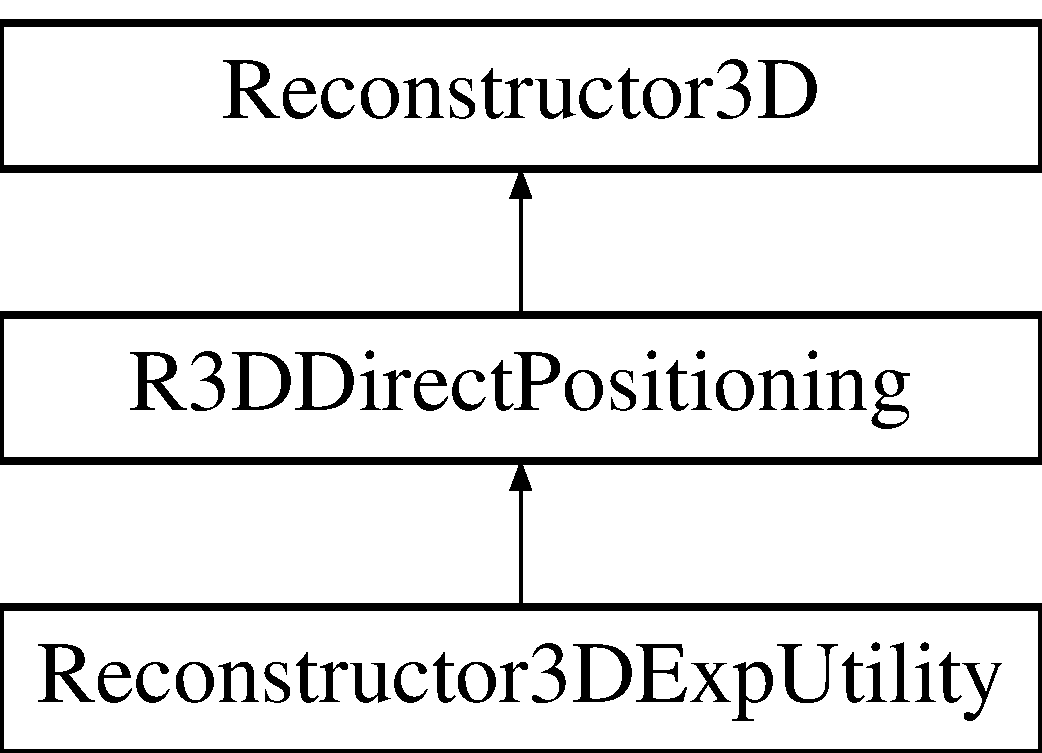
\includegraphics[height=3.000000cm]{classReconstructor3DExpUtility}
\end{center}
\end{figure}
\subsection*{Public Member Functions}
\begin{DoxyCompactItemize}
\item 
{\bfseries Reconstructor3\+D\+Exp\+Utility} (\hyperlink{classRobotSensor}{Robot\+Sensor} $\ast$rs, \hyperlink{classNBVPlanner}{N\+B\+V\+Planner} $\ast$p)\hypertarget{classReconstructor3DExpUtility_af0ba7028b3e96e3a8651f7bf3c585e6d}{}\label{classReconstructor3DExpUtility_af0ba7028b3e96e3a8651f7bf3c585e6d}

\item 
virtual bool {\bfseries positioning} (\hyperlink{classViewStructure}{View\+Structure} v)\hypertarget{classReconstructor3DExpUtility_a1c137e9902abc841e1e955c27a74cbd8}{}\label{classReconstructor3DExpUtility_a1c137e9902abc841e1e955c27a74cbd8}

\end{DoxyCompactItemize}
\subsection*{Additional Inherited Members}


The documentation for this class was generated from the following files\+:\begin{DoxyCompactItemize}
\item 
viewplanning/r3ddirectpositioning.\+h\item 
viewplanning/r3ddirectpositioning.\+cpp\end{DoxyCompactItemize}

\hypertarget{classReconstructor3DRobot}{}\section{Reconstructor3\+D\+Robot Class Reference}
\label{classReconstructor3DRobot}\index{Reconstructor3\+D\+Robot@{Reconstructor3\+D\+Robot}}
Inheritance diagram for Reconstructor3\+D\+Robot\+:\begin{figure}[H]
\begin{center}
\leavevmode
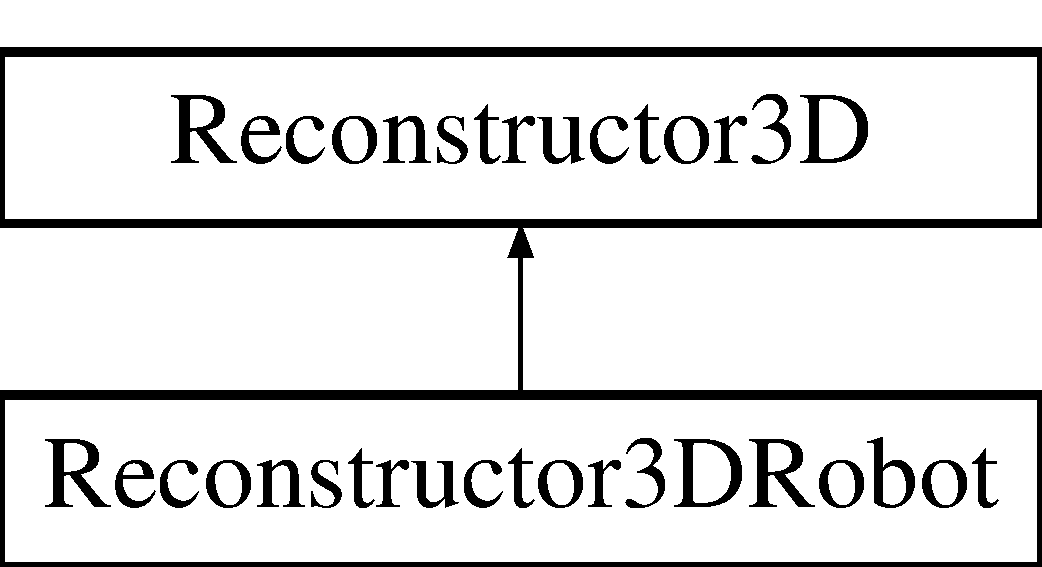
\includegraphics[height=2.000000cm]{classReconstructor3DRobot}
\end{center}
\end{figure}
\subsection*{Public Member Functions}
\begin{DoxyCompactItemize}
\item 
{\bfseries Reconstructor3\+D\+Robot} (\hyperlink{classRobotSensor}{Robot\+Sensor} $\ast$rs, \hyperlink{classNBVPlanner}{N\+B\+V\+Planner} $\ast$p)\hypertarget{classReconstructor3DRobot_ab55aad2f90ffbb721ea928966097599b}{}\label{classReconstructor3DRobot_ab55aad2f90ffbb721ea928966097599b}

\item 
virtual bool {\bfseries positioning} (\hyperlink{classViewStructure}{View\+Structure} v)\hypertarget{classReconstructor3DRobot_ade439094908d055af59c03d604649f02}{}\label{classReconstructor3DRobot_ade439094908d055af59c03d604649f02}

\item 
virtual bool \hyperlink{classReconstructor3DRobot_aa30cad4bf09b5d58cac1e9b751e7842b}{take\+Scan} (std\+::string \&scan\+\_\+name, std\+::string \&origin\+\_\+name)
\item 
virtual bool \hyperlink{classReconstructor3DRobot_abd43d6ee1bb11d843db1d39b7498b1fc}{update\+Model} (std\+::string scan\+\_\+name, std\+::string origin\+\_\+name)
\end{DoxyCompactItemize}
\subsection*{Additional Inherited Members}


\subsection{Member Function Documentation}
\index{Reconstructor3\+D\+Robot@{Reconstructor3\+D\+Robot}!take\+Scan@{take\+Scan}}
\index{take\+Scan@{take\+Scan}!Reconstructor3\+D\+Robot@{Reconstructor3\+D\+Robot}}
\subsubsection[{\texorpdfstring{take\+Scan(std\+::string \&scan\+\_\+name, std\+::string \&origin\+\_\+name)}{takeScan(std::string &scan_name, std::string &origin_name)}}]{\setlength{\rightskip}{0pt plus 5cm}bool Reconstructor3\+D\+Robot\+::take\+Scan (
\begin{DoxyParamCaption}
\item[{std\+::string \&}]{scan\+\_\+name, }
\item[{std\+::string \&}]{origin\+\_\+name}
\end{DoxyParamCaption}
)\hspace{0.3cm}{\ttfamily [virtual]}}\hypertarget{classReconstructor3DRobot_aa30cad4bf09b5d58cac1e9b751e7842b}{}\label{classReconstructor3DRobot_aa30cad4bf09b5d58cac1e9b751e7842b}
Performs a scan and returns the name of the scan file and the origin file 

Reimplemented from \hyperlink{classReconstructor3D_ac4433ce176af00bd57a79d67d0fc4a14}{Reconstructor3D}.

\index{Reconstructor3\+D\+Robot@{Reconstructor3\+D\+Robot}!update\+Model@{update\+Model}}
\index{update\+Model@{update\+Model}!Reconstructor3\+D\+Robot@{Reconstructor3\+D\+Robot}}
\subsubsection[{\texorpdfstring{update\+Model(std\+::string scan\+\_\+name, std\+::string origin\+\_\+name)}{updateModel(std::string scan_name, std::string origin_name)}}]{\setlength{\rightskip}{0pt plus 5cm}bool Reconstructor3\+D\+Robot\+::update\+Model (
\begin{DoxyParamCaption}
\item[{std\+::string}]{scan\+\_\+name, }
\item[{std\+::string}]{origin\+\_\+name}
\end{DoxyParamCaption}
)\hspace{0.3cm}{\ttfamily [virtual]}}\hypertarget{classReconstructor3DRobot_abd43d6ee1bb11d843db1d39b7498b1fc}{}\label{classReconstructor3DRobot_abd43d6ee1bb11d843db1d39b7498b1fc}
convert to P\+CD the initial map

Register the initial map

replace accumulated points

Transform the position of the robot given the computed registration matrix 

Reimplemented from \hyperlink{classReconstructor3D}{Reconstructor3D}.



The documentation for this class was generated from the following files\+:\begin{DoxyCompactItemize}
\item 
viewplanning/r3ddirectpositioning.\+h\item 
viewplanning/r3ddirectpositioning.\+cpp\end{DoxyCompactItemize}

\hypertarget{classRobotSensor}{}\section{Robot\+Sensor Class Reference}
\label{classRobotSensor}\index{Robot\+Sensor@{Robot\+Sensor}}


{\ttfamily \#include $<$robotsensor.\+h$>$}

Inheritance diagram for Robot\+Sensor\+:\begin{figure}[H]
\begin{center}
\leavevmode
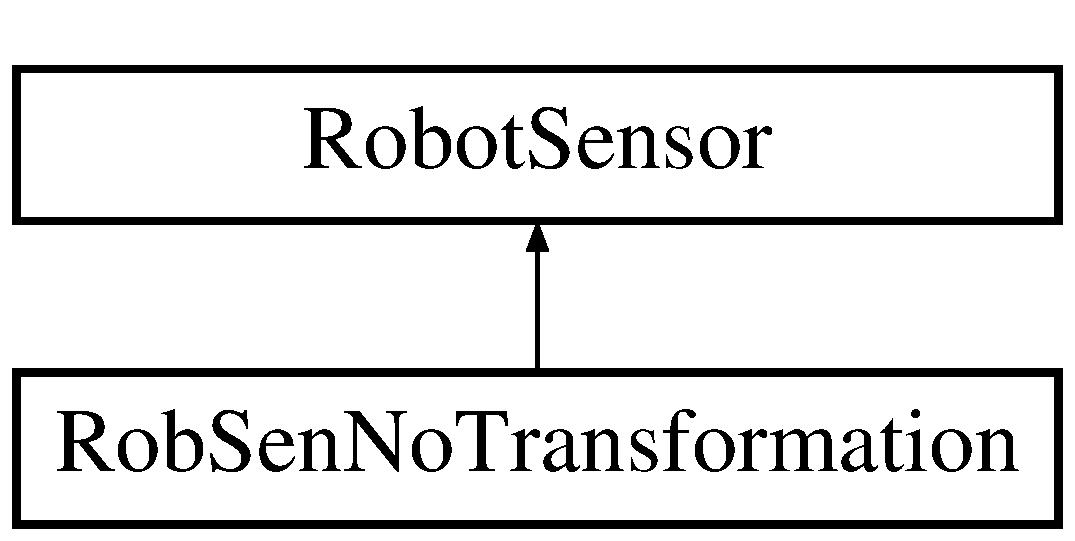
\includegraphics[height=2.000000cm]{classRobotSensor}
\end{center}
\end{figure}
\subsection*{Public Member Functions}
\begin{DoxyCompactItemize}
\item 
{\bfseries Robot\+Sensor} (\hyperlink{classvpRobot}{vp\+Robot} $\ast$r, \hyperlink{classRangeSensor}{Range\+Sensor} $\ast$s)\hypertarget{classRobotSensor_a47be104f6ee7b01bd71641c4ab263073}{}\label{classRobotSensor_a47be104f6ee7b01bd71641c4ab263073}

\item 
virtual long int \hyperlink{classRobotSensor_a76298deca29d80b6543f628f10060bec}{perform\+Scan} ()
\item 
virtual bool {\bfseries init} ()\hypertarget{classRobotSensor_a45bcf4e2911626b8327f29f9bae5de0e}{}\label{classRobotSensor_a45bcf4e2911626b8327f29f9bae5de0e}

\item 
void {\bfseries set\+Config\+Folder} (std\+::string folder)\hypertarget{classRobotSensor_ab528a4acf62f820cd55e2cf149380889}{}\label{classRobotSensor_ab528a4acf62f820cd55e2cf149380889}

\item 
void {\bfseries set\+Data\+Folder} (std\+::string folder)\hypertarget{classRobotSensor_a44fad2d17f516e7cc0e9933dca33fde6}{}\label{classRobotSensor_a44fad2d17f516e7cc0e9933dca33fde6}

\item 
void {\bfseries get\+H\+T\+Mfrom\+Robot} (Boost\+Matrix \&htm\+Robot)\hypertarget{classRobotSensor_a23c00e9c0038943271cf9131daf2099d}{}\label{classRobotSensor_a23c00e9c0038943271cf9131daf2099d}

\item 
void {\bfseries set\+Sensor} (\hyperlink{classRangeSensor}{Range\+Sensor} $\ast$rs)\hypertarget{classRobotSensor_a16703c2dbce8fb189ebadc54302bfd30}{}\label{classRobotSensor_a16703c2dbce8fb189ebadc54302bfd30}

\item 
void \hyperlink{classRobotSensor_ac2095d4f543f88f36cf704414334a2ba}{set\+Sensor\+Pose} (double x, double y, double z, double yaw, double pitch, double roll)
\item 
bool \hyperlink{classRobotSensor_ac832fdd6f319aa6118cf1b3bcbc08394}{save\+Last\+Point\+Cloud} (std\+::string \&file\+\_\+name, double factor)
\item 
bool \hyperlink{classRobotSensor_a05d2aa70583b6a0a87de4f4ab85a64cd}{save\+Last\+Point\+Cloud\+Mts} (std\+::string \&file\+\_\+name)
\item 
bool \hyperlink{classRobotSensor_a03db6a7ccd4accf68f7ae6b28674196a}{save\+Sensor\+Trajectory} (std\+::string \&file\+\_\+name, double factor)
\item 
bool {\bfseries save\+Sensor\+Trajectory\+Mts} (std\+::string \&file\+\_\+name)\hypertarget{classRobotSensor_a5c5e66676a327bcaf318d761a9204ca9}{}\label{classRobotSensor_a5c5e66676a327bcaf318d761a9204ca9}

\item 
void {\bfseries get\+H\+T\+Mfrom\+Sensor} (Boost\+Matrix \&htm\+Sensor)\hypertarget{classRobotSensor_a6b05b86155accadb8dd797eaa6d9ed0c}{}\label{classRobotSensor_a6b05b86155accadb8dd797eaa6d9ed0c}

\item 
void \hyperlink{classRobotSensor_a8d03fa5829bcbfcd9e65461da3a3e88d}{get\+Views\+From\+Comfigurations} (std\+::list$<$ \hyperlink{classViewStructure}{View\+Structure} $>$ \&views)
\item 
void \hyperlink{classRobotSensor_aaadde4cfbe409e2e307916ffe750a64a}{get\+Views\+From\+Comfigurations} (std\+::list$<$ \hyperlink{classViewStructure}{View\+Structure} $>$ \&views, std\+::list$<$ std\+::vector$<$ double $>$ $>$ configurations)
\item 
void \hyperlink{classRobotSensor_a2ba12e8c33f6811634305ee892c2a237}{get\+Random\+State} (std\+::vector$<$ double $>$ \&state)
\item 
void \hyperlink{classRobotSensor_ae7b1b9acbc27b88a365e8a927355e08e}{get\+View\+From\+State} (\hyperlink{classViewStructure}{View\+Structure} \&view, const std\+::vector$<$ double $>$ state)
\item 
bool {\bfseries move\+To\+Configuration} (std\+::vector$<$ double $>$ configuration)\hypertarget{classRobotSensor_ab6fd30a1c23f1ed147eb9597297ae515}{}\label{classRobotSensor_ab6fd30a1c23f1ed147eb9597297ae515}

\item 
bool {\bfseries set\+Path\+To\+Execute} (std\+::vector$<$ std\+::vector$<$ double $>$ $>$ path)\hypertarget{classRobotSensor_a4c5f272ecc68c91880826298857a5457}{}\label{classRobotSensor_a4c5f272ecc68c91880826298857a5457}

\item 
bool {\bfseries set\+Trajectory} (std\+::vector$<$ std\+::vector$<$ double $>$ $>$ trajectory, double delta\+\_\+t)\hypertarget{classRobotSensor_a3c0cef902dea177c28e32a9f505f493f}{}\label{classRobotSensor_a3c0cef902dea177c28e32a9f505f493f}

\item 
bool {\bfseries set\+Goal\+Configuration} (std\+::vector$<$ double $>$ goal\+\_\+q)\hypertarget{classRobotSensor_a639eb18da8934854b3bbb2c468c029ba}{}\label{classRobotSensor_a639eb18da8934854b3bbb2c468c029ba}

\item 
float {\bfseries execute\+Movement} ()\hypertarget{classRobotSensor_af91b4528c7f490ba9236056f4fb9cfd3}{}\label{classRobotSensor_af91b4528c7f490ba9236056f4fb9cfd3}

\item 
void {\bfseries get\+Current\+Configuration} (std\+::vector$<$ double $>$ \&configuration)\hypertarget{classRobotSensor_a4b7a23f169416d68ca709305bab109c9}{}\label{classRobotSensor_a4b7a23f169416d68ca709305bab109c9}

\item 
bool \hyperlink{classRobotSensor_a8cfdb150fb9a8add2df06009c258e139}{update\+Robot\+Localization} (mrpt\+::poses\+::\+C\+Pose3D transformation)\hypertarget{classRobotSensor_a8cfdb150fb9a8add2df06009c258e139}{}\label{classRobotSensor_a8cfdb150fb9a8add2df06009c258e139}

\begin{DoxyCompactList}\small\item\em updates the configuration of the robot with a transformation. Usually this trasnformation is obtained by the Registration process. \end{DoxyCompactList}\item 
virtual bool \hyperlink{classRobotSensor_a8e1c363f54f6e5a00499b93fd245a3da}{auto\+Occlusion} (std\+::vector$<$ double $>$ q)
\item 
virtual bool \hyperlink{classRobotSensor_a720b3046a49b028d07090c1c79cd0a96}{points\+To\+The\+Robot} (\hyperlink{classViewStructure}{View\+Structure} view, std\+::vector$<$ double $>$ q)
\end{DoxyCompactItemize}
\subsection*{Protected Member Functions}
\begin{DoxyCompactItemize}
\item 
void {\bfseries convert\+Points\+To\+Robot\+Reference} (std\+::vector$<$ mrpt\+::poses\+::\+C\+Point3D $>$ \&points, std\+::vector$<$ mrpt\+::poses\+::\+C\+Point3D $>$ \&result)\hypertarget{classRobotSensor_a5c36e17b54e0f4c06cd3b47e8976c924}{}\label{classRobotSensor_a5c36e17b54e0f4c06cd3b47e8976c924}

\item 
void {\bfseries add\+Points\+To\+Point\+Cloud} (std\+::vector$<$ mrpt\+::poses\+::\+C\+Point3D $>$ \&points, std\+::vector$<$ mrpt\+::poses\+::\+C\+Point3D $>$ \&origins, bool clear=true)\hypertarget{classRobotSensor_a317e3af77772a792ac4672f0461d2da8}{}\label{classRobotSensor_a317e3af77772a792ac4672f0461d2da8}

\item 
double {\bfseries dot\+Product} (mrpt\+::poses\+::\+C\+Point3D a, mrpt\+::poses\+::\+C\+Point3D b)\hypertarget{classRobotSensor_a548c1dd9588bad4f1a3d8a4aa96c7fbe}{}\label{classRobotSensor_a548c1dd9588bad4f1a3d8a4aa96c7fbe}

\end{DoxyCompactItemize}
\subsection*{Protected Attributes}
\begin{DoxyCompactItemize}
\item 
\hyperlink{classRangeSensor}{Range\+Sensor} $\ast$ {\bfseries sensor}\hypertarget{classRobotSensor_ac00737b26fc36d09497491988f6575e8}{}\label{classRobotSensor_ac00737b26fc36d09497491988f6575e8}

\item 
\hyperlink{classvpRobot}{vp\+Robot} $\ast$ {\bfseries robot}\hypertarget{classRobotSensor_ab416376e6423bb05d0d938eda2875b83}{}\label{classRobotSensor_ab416376e6423bb05d0d938eda2875b83}

\item 
std\+::string {\bfseries config\+Folder}\hypertarget{classRobotSensor_a3014b0bc086158cdbe1aca964f291b9a}{}\label{classRobotSensor_a3014b0bc086158cdbe1aca964f291b9a}

\item 
std\+::string {\bfseries data\+Folder}\hypertarget{classRobotSensor_a7c4a87715cac0b18bc7281cd3b0fa2fe}{}\label{classRobotSensor_a7c4a87715cac0b18bc7281cd3b0fa2fe}

\item 
std\+::vector$<$ double $>$ \hyperlink{classRobotSensor_a7e9d4be5f206d56109fc2e3c34e2aac2}{sensor\+Pose}
\item 
mrpt\+::poses\+::\+C\+Pose3D \hyperlink{classRobotSensor_a88bbdab74a1836ca367bcb344c4ca241}{Sensor\+Pose}
\item 
std\+::list$<$ mrpt\+::poses\+::\+C\+Point3D $>$ \hyperlink{classRobotSensor_a06d39a90daef29d623424b3608e0ee7b}{point\+Cloud}
\item 
uint32\+\_\+t \hyperlink{classRobotSensor_ae111af80a4feac4eb9ce0fbf740777c2}{point\+Cloud\+Id\+Counter}
\item 
std\+::list$<$ mrpt\+::poses\+::\+C\+Point3D $>$ \hyperlink{classRobotSensor_a47898d707a343c7530018493c87f3320}{Sensor\+Trajectory}
\item 
bool {\bfseries sensor\+Ready}\hypertarget{classRobotSensor_acaa1d9e26d7c609dc8374f1d1e474435}{}\label{classRobotSensor_acaa1d9e26d7c609dc8374f1d1e474435}

\item 
bool {\bfseries robot\+Ready}\hypertarget{classRobotSensor_a52448933140efcd8f8565ab02712fab4}{}\label{classRobotSensor_a52448933140efcd8f8565ab02712fab4}

\end{DoxyCompactItemize}


\subsection{Detailed Description}
Clase base that represents a robot with a range sensor mounted on it. With this we can perform scans and save them to the Robot coordinate reference. Requires a robot and a sensor 

\subsection{Member Function Documentation}
\index{Robot\+Sensor@{Robot\+Sensor}!auto\+Occlusion@{auto\+Occlusion}}
\index{auto\+Occlusion@{auto\+Occlusion}!Robot\+Sensor@{Robot\+Sensor}}
\subsubsection[{\texorpdfstring{auto\+Occlusion(std\+::vector$<$ double $>$ q)}{autoOcclusion(std::vector< double > q)}}]{\setlength{\rightskip}{0pt plus 5cm}bool Robot\+Sensor\+::auto\+Occlusion (
\begin{DoxyParamCaption}
\item[{std\+::vector$<$ double $>$}]{q}
\end{DoxyParamCaption}
)\hspace{0.3cm}{\ttfamily [virtual]}}\hypertarget{classRobotSensor_a8e1c363f54f6e5a00499b93fd245a3da}{}\label{classRobotSensor_a8e1c363f54f6e5a00499b93fd245a3da}
verificar si el rayo director del sensor intersecta con el robot en determinada configuración \index{Robot\+Sensor@{Robot\+Sensor}!get\+Random\+State@{get\+Random\+State}}
\index{get\+Random\+State@{get\+Random\+State}!Robot\+Sensor@{Robot\+Sensor}}
\subsubsection[{\texorpdfstring{get\+Random\+State(std\+::vector$<$ double $>$ \&state)}{getRandomState(std::vector< double > &state)}}]{\setlength{\rightskip}{0pt plus 5cm}void Robot\+Sensor\+::get\+Random\+State (
\begin{DoxyParamCaption}
\item[{std\+::vector$<$ double $>$ \&}]{state}
\end{DoxyParamCaption}
)}\hypertarget{classRobotSensor_a2ba12e8c33f6811634305ee892c2a237}{}\label{classRobotSensor_a2ba12e8c33f6811634305ee892c2a237}
Gets a random state between lower and upper states \index{Robot\+Sensor@{Robot\+Sensor}!get\+View\+From\+State@{get\+View\+From\+State}}
\index{get\+View\+From\+State@{get\+View\+From\+State}!Robot\+Sensor@{Robot\+Sensor}}
\subsubsection[{\texorpdfstring{get\+View\+From\+State(\+View\+Structure \&view, const std\+::vector$<$ double $>$ state)}{getViewFromState(ViewStructure &view, const std::vector< double > state)}}]{\setlength{\rightskip}{0pt plus 5cm}void Robot\+Sensor\+::get\+View\+From\+State (
\begin{DoxyParamCaption}
\item[{{\bf View\+Structure} \&}]{view, }
\item[{const std\+::vector$<$ double $>$}]{state}
\end{DoxyParamCaption}
)}\hypertarget{classRobotSensor_ae7b1b9acbc27b88a365e8a927355e08e}{}\label{classRobotSensor_ae7b1b9acbc27b88a365e8a927355e08e}
Gets a View structure from a state \index{Robot\+Sensor@{Robot\+Sensor}!get\+Views\+From\+Comfigurations@{get\+Views\+From\+Comfigurations}}
\index{get\+Views\+From\+Comfigurations@{get\+Views\+From\+Comfigurations}!Robot\+Sensor@{Robot\+Sensor}}
\subsubsection[{\texorpdfstring{get\+Views\+From\+Comfigurations(std\+::list$<$ View\+Structure $>$ \&views)}{getViewsFromComfigurations(std::list< ViewStructure > &views)}}]{\setlength{\rightskip}{0pt plus 5cm}void Robot\+Sensor\+::get\+Views\+From\+Comfigurations (
\begin{DoxyParamCaption}
\item[{std\+::list$<$ {\bf View\+Structure} $>$ \&}]{views}
\end{DoxyParamCaption}
)}\hypertarget{classRobotSensor_a8d03fa5829bcbfcd9e65461da3a3e88d}{}\label{classRobotSensor_a8d03fa5829bcbfcd9e65461da3a3e88d}
N\+O\+TE\+: this is only a patch!!!! Receives a set of configurations in views format. Only the vector q is taken into account. Returns the same set of views but with H\+TM filled. You can also use a get\+Views\+From\+Comfigurations \index{Robot\+Sensor@{Robot\+Sensor}!get\+Views\+From\+Comfigurations@{get\+Views\+From\+Comfigurations}}
\index{get\+Views\+From\+Comfigurations@{get\+Views\+From\+Comfigurations}!Robot\+Sensor@{Robot\+Sensor}}
\subsubsection[{\texorpdfstring{get\+Views\+From\+Comfigurations(std\+::list$<$ View\+Structure $>$ \&views, std\+::list$<$ std\+::vector$<$ double $>$ $>$ configurations)}{getViewsFromComfigurations(std::list< ViewStructure > &views, std::list< std::vector< double > > configurations)}}]{\setlength{\rightskip}{0pt plus 5cm}void Robot\+Sensor\+::get\+Views\+From\+Comfigurations (
\begin{DoxyParamCaption}
\item[{std\+::list$<$ {\bf View\+Structure} $>$ \&}]{views, }
\item[{std\+::list$<$ std\+::vector$<$ double $>$ $>$}]{configurations}
\end{DoxyParamCaption}
)}\hypertarget{classRobotSensor_aaadde4cfbe409e2e307916ffe750a64a}{}\label{classRobotSensor_aaadde4cfbe409e2e307916ffe750a64a}
Receives a set of configurations and returns a set of views. A view include besides the configuration, the Homogenous Transformation Matrix in Workspace \index{Robot\+Sensor@{Robot\+Sensor}!perform\+Scan@{perform\+Scan}}
\index{perform\+Scan@{perform\+Scan}!Robot\+Sensor@{Robot\+Sensor}}
\subsubsection[{\texorpdfstring{perform\+Scan()}{performScan()}}]{\setlength{\rightskip}{0pt plus 5cm}long int Robot\+Sensor\+::perform\+Scan (
\begin{DoxyParamCaption}
{}
\end{DoxyParamCaption}
)\hspace{0.3cm}{\ttfamily [virtual]}}\hypertarget{classRobotSensor_a76298deca29d80b6543f628f10060bec}{}\label{classRobotSensor_a76298deca29d80b6543f628f10060bec}
Performs a scan at current position 

Reimplemented in \hyperlink{classRobSenNoTransformation_a1fe9d3c79ea7e29892c58792b1fa05d8}{Rob\+Sen\+No\+Transformation}.

\index{Robot\+Sensor@{Robot\+Sensor}!points\+To\+The\+Robot@{points\+To\+The\+Robot}}
\index{points\+To\+The\+Robot@{points\+To\+The\+Robot}!Robot\+Sensor@{Robot\+Sensor}}
\subsubsection[{\texorpdfstring{points\+To\+The\+Robot(\+View\+Structure view, std\+::vector$<$ double $>$ q)}{pointsToTheRobot(ViewStructure view, std::vector< double > q)}}]{\setlength{\rightskip}{0pt plus 5cm}bool Robot\+Sensor\+::points\+To\+The\+Robot (
\begin{DoxyParamCaption}
\item[{{\bf View\+Structure}}]{view, }
\item[{std\+::vector$<$ double $>$}]{q}
\end{DoxyParamCaption}
)\hspace{0.3cm}{\ttfamily [virtual]}}\hypertarget{classRobotSensor_a720b3046a49b028d07090c1c79cd0a96}{}\label{classRobotSensor_a720b3046a49b028d07090c1c79cd0a96}
Esto debería hacerse tomando en cuenta la forma del robot Sin embargo por tiempo de implementación solo se verifica si intersecta una esfera que representa el robot\index{Robot\+Sensor@{Robot\+Sensor}!save\+Last\+Point\+Cloud@{save\+Last\+Point\+Cloud}}
\index{save\+Last\+Point\+Cloud@{save\+Last\+Point\+Cloud}!Robot\+Sensor@{Robot\+Sensor}}
\subsubsection[{\texorpdfstring{save\+Last\+Point\+Cloud(std\+::string \&file\+\_\+name, double factor)}{saveLastPointCloud(std::string &file_name, double factor)}}]{\setlength{\rightskip}{0pt plus 5cm}bool Robot\+Sensor\+::save\+Last\+Point\+Cloud (
\begin{DoxyParamCaption}
\item[{std\+::string \&}]{file\+\_\+name, }
\item[{double}]{factor}
\end{DoxyParamCaption}
)}\hypertarget{classRobotSensor_ac832fdd6f319aa6118cf1b3bcbc08394}{}\label{classRobotSensor_ac832fdd6f319aa6118cf1b3bcbc08394}
Saves the last point cloud. Adds the folder and the extension. \index{Robot\+Sensor@{Robot\+Sensor}!save\+Last\+Point\+Cloud\+Mts@{save\+Last\+Point\+Cloud\+Mts}}
\index{save\+Last\+Point\+Cloud\+Mts@{save\+Last\+Point\+Cloud\+Mts}!Robot\+Sensor@{Robot\+Sensor}}
\subsubsection[{\texorpdfstring{save\+Last\+Point\+Cloud\+Mts(std\+::string \&file\+\_\+name)}{saveLastPointCloudMts(std::string &file_name)}}]{\setlength{\rightskip}{0pt plus 5cm}bool Robot\+Sensor\+::save\+Last\+Point\+Cloud\+Mts (
\begin{DoxyParamCaption}
\item[{std\+::string \&}]{file\+\_\+name}
\end{DoxyParamCaption}
)}\hypertarget{classRobotSensor_a05d2aa70583b6a0a87de4f4ab85a64cd}{}\label{classRobotSensor_a05d2aa70583b6a0a87de4f4ab85a64cd}
Saves the last point cloud in a raw text file (mts). The file will have the name \char`\"{}scan\+\_\+\mbox{[}number\+\_\+of\+\_\+scan\mbox{]}.\+dat\char`\"{} and it will be saved at the folder specified by problem Adress. \index{Robot\+Sensor@{Robot\+Sensor}!save\+Sensor\+Trajectory@{save\+Sensor\+Trajectory}}
\index{save\+Sensor\+Trajectory@{save\+Sensor\+Trajectory}!Robot\+Sensor@{Robot\+Sensor}}
\subsubsection[{\texorpdfstring{save\+Sensor\+Trajectory(std\+::string \&file\+\_\+name, double factor)}{saveSensorTrajectory(std::string &file_name, double factor)}}]{\setlength{\rightskip}{0pt plus 5cm}bool Robot\+Sensor\+::save\+Sensor\+Trajectory (
\begin{DoxyParamCaption}
\item[{std\+::string \&}]{file\+\_\+name, }
\item[{double}]{factor}
\end{DoxyParamCaption}
)}\hypertarget{classRobotSensor_a03db6a7ccd4accf68f7ae6b28674196a}{}\label{classRobotSensor_a03db6a7ccd4accf68f7ae6b28674196a}
Saves the origins of the scans. Adds the folder and extension automaticly. \index{Robot\+Sensor@{Robot\+Sensor}!set\+Sensor\+Pose@{set\+Sensor\+Pose}}
\index{set\+Sensor\+Pose@{set\+Sensor\+Pose}!Robot\+Sensor@{Robot\+Sensor}}
\subsubsection[{\texorpdfstring{set\+Sensor\+Pose(double x, double y, double z, double yaw, double pitch, double roll)}{setSensorPose(double x, double y, double z, double yaw, double pitch, double roll)}}]{\setlength{\rightskip}{0pt plus 5cm}void Robot\+Sensor\+::set\+Sensor\+Pose (
\begin{DoxyParamCaption}
\item[{double}]{x, }
\item[{double}]{y, }
\item[{double}]{z, }
\item[{double}]{yaw, }
\item[{double}]{pitch, }
\item[{double}]{roll}
\end{DoxyParamCaption}
)}\hypertarget{classRobotSensor_ac2095d4f543f88f36cf704414334a2ba}{}\label{classRobotSensor_ac2095d4f543f88f36cf704414334a2ba}
I\+M\+P\+O\+R\+T\+A\+NT\+: yaw is rotation over Z pitch is a rotation over Y roll is a rotation over X radians 

\subsection{Member Data Documentation}
\index{Robot\+Sensor@{Robot\+Sensor}!point\+Cloud@{point\+Cloud}}
\index{point\+Cloud@{point\+Cloud}!Robot\+Sensor@{Robot\+Sensor}}
\subsubsection[{\texorpdfstring{point\+Cloud}{pointCloud}}]{\setlength{\rightskip}{0pt plus 5cm}std\+::list$<$mrpt\+::poses\+::\+C\+Point3D$>$ Robot\+Sensor\+::point\+Cloud\hspace{0.3cm}{\ttfamily [protected]}}\hypertarget{classRobotSensor_a06d39a90daef29d623424b3608e0ee7b}{}\label{classRobotSensor_a06d39a90daef29d623424b3608e0ee7b}
The last captured point cloud. \index{Robot\+Sensor@{Robot\+Sensor}!point\+Cloud\+Id\+Counter@{point\+Cloud\+Id\+Counter}}
\index{point\+Cloud\+Id\+Counter@{point\+Cloud\+Id\+Counter}!Robot\+Sensor@{Robot\+Sensor}}
\subsubsection[{\texorpdfstring{point\+Cloud\+Id\+Counter}{pointCloudIdCounter}}]{\setlength{\rightskip}{0pt plus 5cm}uint32\+\_\+t Robot\+Sensor\+::point\+Cloud\+Id\+Counter\hspace{0.3cm}{\ttfamily [protected]}}\hypertarget{classRobotSensor_ae111af80a4feac4eb9ce0fbf740777c2}{}\label{classRobotSensor_ae111af80a4feac4eb9ce0fbf740777c2}
Counter for the captured point clouds. \index{Robot\+Sensor@{Robot\+Sensor}!sensor\+Pose@{sensor\+Pose}}
\index{sensor\+Pose@{sensor\+Pose}!Robot\+Sensor@{Robot\+Sensor}}
\subsubsection[{\texorpdfstring{sensor\+Pose}{sensorPose}}]{\setlength{\rightskip}{0pt plus 5cm}std\+::vector$<$double$>$ Robot\+Sensor\+::sensor\+Pose\hspace{0.3cm}{\ttfamily [protected]}}\hypertarget{classRobotSensor_a7e9d4be5f206d56109fc2e3c34e2aac2}{}\label{classRobotSensor_a7e9d4be5f206d56109fc2e3c34e2aac2}
I\+M\+P\+O\+R\+T\+A\+NT\+: yaw is rotation over Z pitch is a rotation over Y roll is a rotation over X \index{Robot\+Sensor@{Robot\+Sensor}!Sensor\+Pose@{Sensor\+Pose}}
\index{Sensor\+Pose@{Sensor\+Pose}!Robot\+Sensor@{Robot\+Sensor}}
\subsubsection[{\texorpdfstring{Sensor\+Pose}{SensorPose}}]{\setlength{\rightskip}{0pt plus 5cm}mrpt\+::poses\+::\+C\+Pose3D Robot\+Sensor\+::\+Sensor\+Pose\hspace{0.3cm}{\ttfamily [protected]}}\hypertarget{classRobotSensor_a88bbdab74a1836ca367bcb344c4ca241}{}\label{classRobotSensor_a88bbdab74a1836ca367bcb344c4ca241}
Sensor pose respect to the Robot \index{Robot\+Sensor@{Robot\+Sensor}!Sensor\+Trajectory@{Sensor\+Trajectory}}
\index{Sensor\+Trajectory@{Sensor\+Trajectory}!Robot\+Sensor@{Robot\+Sensor}}
\subsubsection[{\texorpdfstring{Sensor\+Trajectory}{SensorTrajectory}}]{\setlength{\rightskip}{0pt plus 5cm}std\+::list$<$mrpt\+::poses\+::\+C\+Point3D$>$ Robot\+Sensor\+::\+Sensor\+Trajectory\hspace{0.3cm}{\ttfamily [protected]}}\hypertarget{classRobotSensor_a47898d707a343c7530018493c87f3320}{}\label{classRobotSensor_a47898d707a343c7530018493c87f3320}
Trajectory of the sensor (if there was a sweeping) or origin in cases of a 3D sensor 

The documentation for this class was generated from the following files\+:\begin{DoxyCompactItemize}
\item 
viewplanning/robotsensor.\+h\item 
viewplanning/robotsensor.\+cpp\end{DoxyCompactItemize}

\hypertarget{classRobSenNoTransformation}{}\section{Rob\+Sen\+No\+Transformation Class Reference}
\label{classRobSenNoTransformation}\index{Rob\+Sen\+No\+Transformation@{Rob\+Sen\+No\+Transformation}}
Inheritance diagram for Rob\+Sen\+No\+Transformation\+:\begin{figure}[H]
\begin{center}
\leavevmode
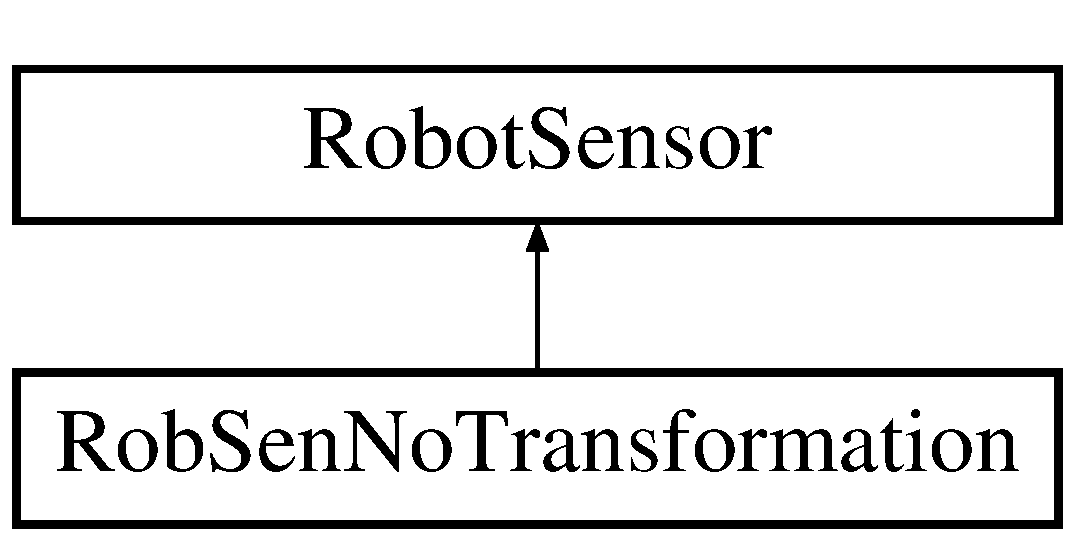
\includegraphics[height=2.000000cm]{classRobSenNoTransformation}
\end{center}
\end{figure}
\subsection*{Public Member Functions}
\begin{DoxyCompactItemize}
\item 
{\bfseries Rob\+Sen\+No\+Transformation} (\hyperlink{classvpRobot}{vp\+Robot} $\ast$r, \hyperlink{classRangeSensor}{Range\+Sensor} $\ast$s)\hypertarget{classRobSenNoTransformation_a4922f5c63d5c2d39f0c8c7bccefa315e}{}\label{classRobSenNoTransformation_a4922f5c63d5c2d39f0c8c7bccefa315e}

\item 
virtual long int \hyperlink{classRobSenNoTransformation_a1fe9d3c79ea7e29892c58792b1fa05d8}{perform\+Scan} ()
\end{DoxyCompactItemize}
\subsection*{Additional Inherited Members}


\subsection{Member Function Documentation}
\index{Rob\+Sen\+No\+Transformation@{Rob\+Sen\+No\+Transformation}!perform\+Scan@{perform\+Scan}}
\index{perform\+Scan@{perform\+Scan}!Rob\+Sen\+No\+Transformation@{Rob\+Sen\+No\+Transformation}}
\subsubsection[{\texorpdfstring{perform\+Scan()}{performScan()}}]{\setlength{\rightskip}{0pt plus 5cm}long int Rob\+Sen\+No\+Transformation\+::perform\+Scan (
\begin{DoxyParamCaption}
{}
\end{DoxyParamCaption}
)\hspace{0.3cm}{\ttfamily [virtual]}}\hypertarget{classRobSenNoTransformation_a1fe9d3c79ea7e29892c58792b1fa05d8}{}\label{classRobSenNoTransformation_a1fe9d3c79ea7e29892c58792b1fa05d8}
Performs a scan at current position 

Reimplemented from \hyperlink{classRobotSensor_a76298deca29d80b6543f628f10060bec}{Robot\+Sensor}.



The documentation for this class was generated from the following files\+:\begin{DoxyCompactItemize}
\item 
viewplanning/robsennotransformation.\+h\item 
viewplanning/robsennotransformation.\+cpp\end{DoxyCompactItemize}

\hypertarget{classViewList}{}\section{View\+List Class Reference}
\label{classViewList}\index{View\+List@{View\+List}}
Inheritance diagram for View\+List\+:\begin{figure}[H]
\begin{center}
\leavevmode
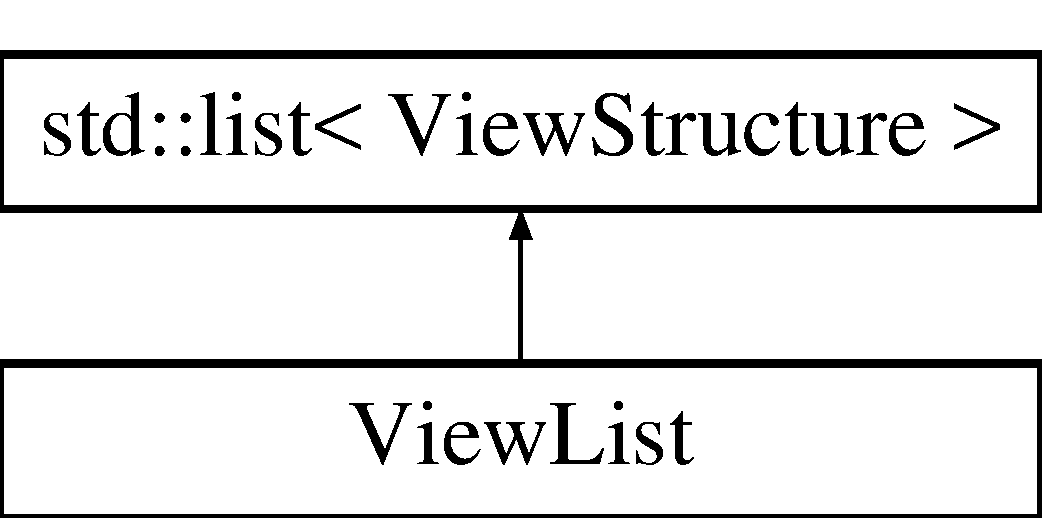
\includegraphics[height=2.000000cm]{classViewList}
\end{center}
\end{figure}
\subsection*{Public Member Functions}
\begin{DoxyCompactItemize}
\item 
bool {\bfseries save} (std\+::string file\+\_\+name)\hypertarget{classViewList_a2d5e411130ffff034c19b94e36d1d794}{}\label{classViewList_a2d5e411130ffff034c19b94e36d1d794}

\item 
bool {\bfseries save\+As\+M\+S\+L\+States} (std\+::string file\+\_\+name)\hypertarget{classViewList_aaf8953fb8a9a7ef1ff5aef717be9ef83}{}\label{classViewList_aaf8953fb8a9a7ef1ff5aef717be9ef83}

\item 
bool {\bfseries read} (std\+::string file\+\_\+name)\hypertarget{classViewList_aa696263f92488a5d8b2111619b628c20}{}\label{classViewList_aa696263f92488a5d8b2111619b628c20}

\item 
\hyperlink{classViewStructure}{View\+Structure} {\bfseries get\+Best\+View} ()\hypertarget{classViewList_a1e7373f6950ca214bc009ed08035e2d3}{}\label{classViewList_a1e7373f6950ca214bc009ed08035e2d3}

\item 
void {\bfseries sort\+High\+To\+Low} ()\hypertarget{classViewList_ab95513795727188e63a18c8cff09f451}{}\label{classViewList_ab95513795727188e63a18c8cff09f451}

\end{DoxyCompactItemize}


The documentation for this class was generated from the following files\+:\begin{DoxyCompactItemize}
\item 
partialmodel/viewstructure.\+h\item 
partialmodel/viewstructure.\+cpp\end{DoxyCompactItemize}

\hypertarget{classViewSphereSynthesis}{}\section{View\+Sphere\+Synthesis Class Reference}
\label{classViewSphereSynthesis}\index{View\+Sphere\+Synthesis@{View\+Sphere\+Synthesis}}
Inheritance diagram for View\+Sphere\+Synthesis\+:\begin{figure}[H]
\begin{center}
\leavevmode
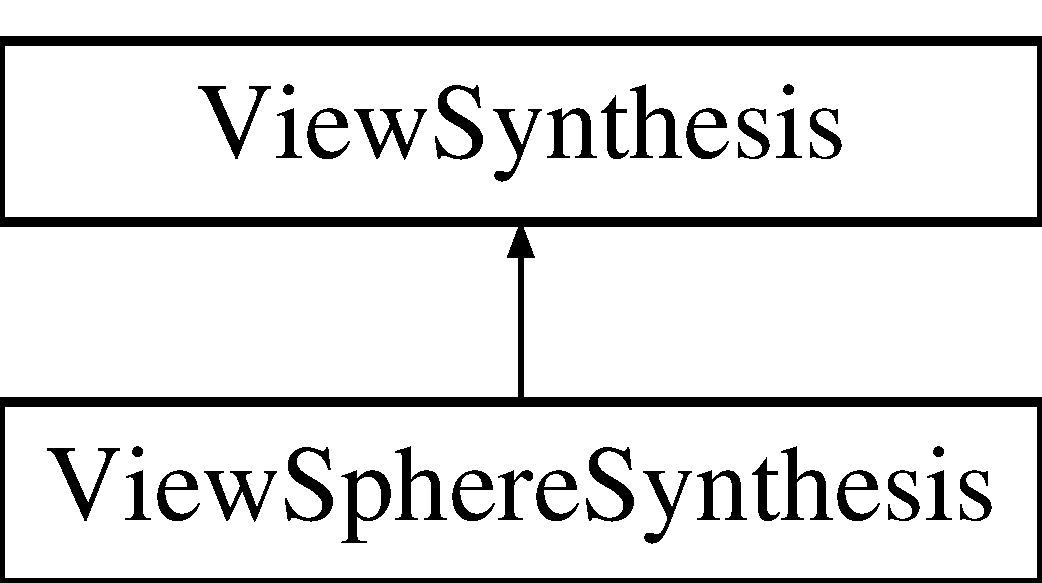
\includegraphics[height=2.000000cm]{classViewSphereSynthesis}
\end{center}
\end{figure}
\subsection*{Public Member Functions}
\begin{DoxyCompactItemize}
\item 
{\bfseries View\+Sphere\+Synthesis} (double r, double x, double y, double z, int level=1)\hypertarget{classViewSphereSynthesis_a840f30a912c0bf9c79b31b337561fbc4}{}\label{classViewSphereSynthesis_a840f30a912c0bf9c79b31b337561fbc4}

\item 
virtual void {\bfseries get\+Views} (\hyperlink{classViewList}{View\+List} \&views)\hypertarget{classViewSphereSynthesis_aa3d9003ac3ebe5ee344d287f2390baa1}{}\label{classViewSphereSynthesis_aa3d9003ac3ebe5ee344d287f2390baa1}

\end{DoxyCompactItemize}
\subsection*{Protected Member Functions}
\begin{DoxyCompactItemize}
\item 
int \hyperlink{classViewSphereSynthesis_a50eae8cee2974cff4146045350f67eca}{get\+Sphere\+Positions\+By\+Tesselation} (int level, std\+::vector$<$ std\+::vector$<$ double $>$ $>$ \&points)
\item 
void {\bfseries init\+Icosahedro} ()\hypertarget{classViewSphereSynthesis_a04931cdc9640c27bd26525e814671d46}{}\label{classViewSphereSynthesis_a04931cdc9640c27bd26525e814671d46}

\item 
void {\bfseries subdivide} ()\hypertarget{classViewSphereSynthesis_a310ae6760ebd0cc7fcbd67d0bb54ce62}{}\label{classViewSphereSynthesis_a310ae6760ebd0cc7fcbd67d0bb54ce62}

\item 
int {\bfseries midpoint\+Search} (int index\+\_\+start, int index\+\_\+end)\hypertarget{classViewSphereSynthesis_ade7009b22f617a15a6c9491c04745a27}{}\label{classViewSphereSynthesis_ade7009b22f617a15a6c9491c04745a27}

\item 
void {\bfseries copy\+Sphere} (std\+::vector$<$ std\+::vector$<$ double $>$ $>$ \&points)\hypertarget{classViewSphereSynthesis_ac50918827f0afa2f58181421508e5394}{}\label{classViewSphereSynthesis_ac50918827f0afa2f58181421508e5394}

\item 
float $\ast$$\ast$ {\bfseries m\+F\+Matrix} (int nrl, int nrh, int ncl, int nch)\hypertarget{classViewSphereSynthesis_abb1d9052489b453ac23d07fc48ff6944}{}\label{classViewSphereSynthesis_abb1d9052489b453ac23d07fc48ff6944}

\item 
void {\bfseries m\+Free\+F\+Matrix} (float $\ast$$\ast$m, int nrl, int nrh, int ncl, int nch)\hypertarget{classViewSphereSynthesis_acce1929f0ceede5231334e4e8394a017}{}\label{classViewSphereSynthesis_acce1929f0ceede5231334e4e8394a017}

\item 
void \hyperlink{classViewSphereSynthesis_a98fe600fc19d8778f5d21b458a880468}{get\+Pointed\+Views} (std\+::vector$<$ std\+::vector$<$ double $>$ $>$ points, \hyperlink{classViewList}{View\+List} \&views)
\end{DoxyCompactItemize}
\subsection*{Protected Attributes}
\begin{DoxyCompactItemize}
\item 
double {\bfseries radius}\hypertarget{classViewSphereSynthesis_a3beee84f46a4a0c097d79e72267ead55}{}\label{classViewSphereSynthesis_a3beee84f46a4a0c097d79e72267ead55}

\item 
double {\bfseries cx}\hypertarget{classViewSphereSynthesis_a33a1a1b8ce90866b821ff223751a132e}{}\label{classViewSphereSynthesis_a33a1a1b8ce90866b821ff223751a132e}

\item 
double {\bfseries cy}\hypertarget{classViewSphereSynthesis_a104db3286f62521e501f5367c4643153}{}\label{classViewSphereSynthesis_a104db3286f62521e501f5367c4643153}

\item 
double {\bfseries cz}\hypertarget{classViewSphereSynthesis_a05b06a7980d8d81294c4852a43601936}{}\label{classViewSphereSynthesis_a05b06a7980d8d81294c4852a43601936}

\item 
int {\bfseries tesselation\+\_\+level}\hypertarget{classViewSphereSynthesis_ab714a7f99b7b4e795a8cca8147b8abda}{}\label{classViewSphereSynthesis_ab714a7f99b7b4e795a8cca8147b8abda}

\item 
int {\bfseries n\+\_\+vertices}\hypertarget{classViewSphereSynthesis_a23cc8863a4eaadd53ef753d5e5d7ee93}{}\label{classViewSphereSynthesis_a23cc8863a4eaadd53ef753d5e5d7ee93}

\item 
int {\bfseries n\+\_\+faces}\hypertarget{classViewSphereSynthesis_a62890a53dcd8668e848c01ca8b2ca495}{}\label{classViewSphereSynthesis_a62890a53dcd8668e848c01ca8b2ca495}

\item 
int {\bfseries n\+\_\+edges}\hypertarget{classViewSphereSynthesis_a1af416e731572cf6cf8002d5e35e6c7a}{}\label{classViewSphereSynthesis_a1af416e731572cf6cf8002d5e35e6c7a}

\item 
float $\ast$ {\bfseries vertices}\hypertarget{classViewSphereSynthesis_afe1289b0c5b222b9d60cd7ab6b45264b}{}\label{classViewSphereSynthesis_afe1289b0c5b222b9d60cd7ab6b45264b}

\item 
int $\ast$ {\bfseries faces}\hypertarget{classViewSphereSynthesis_a87633500eb5be257ebee7a2130273589}{}\label{classViewSphereSynthesis_a87633500eb5be257ebee7a2130273589}

\item 
int {\bfseries edge\+\_\+run}\hypertarget{classViewSphereSynthesis_a22f4c0222e606ae9615a9499d0e3ec47}{}\label{classViewSphereSynthesis_a22f4c0222e606ae9615a9499d0e3ec47}

\item 
int $\ast$ {\bfseries start}\hypertarget{classViewSphereSynthesis_a5c6464a7ac1131c22347c958ea217bd3}{}\label{classViewSphereSynthesis_a5c6464a7ac1131c22347c958ea217bd3}

\item 
int $\ast$ {\bfseries end}\hypertarget{classViewSphereSynthesis_a48936083e43fdc7b05f22197edb81852}{}\label{classViewSphereSynthesis_a48936083e43fdc7b05f22197edb81852}

\item 
int $\ast$ {\bfseries midpoint}\hypertarget{classViewSphereSynthesis_a44f73c9767ee986d3b523b32a3ae0395}{}\label{classViewSphereSynthesis_a44f73c9767ee986d3b523b32a3ae0395}

\end{DoxyCompactItemize}


\subsection{Member Function Documentation}
\index{View\+Sphere\+Synthesis@{View\+Sphere\+Synthesis}!get\+Pointed\+Views@{get\+Pointed\+Views}}
\index{get\+Pointed\+Views@{get\+Pointed\+Views}!View\+Sphere\+Synthesis@{View\+Sphere\+Synthesis}}
\subsubsection[{\texorpdfstring{get\+Pointed\+Views(std\+::vector$<$ std\+::vector$<$ double $>$ $>$ points, View\+List \&views)}{getPointedViews(std::vector< std::vector< double > > points, ViewList &views)}}]{\setlength{\rightskip}{0pt plus 5cm}void View\+Sphere\+Synthesis\+::get\+Pointed\+Views (
\begin{DoxyParamCaption}
\item[{std\+::vector$<$ std\+::vector$<$ double $>$ $>$}]{points, }
\item[{{\bf View\+List} \&}]{views}
\end{DoxyParamCaption}
)\hspace{0.3cm}{\ttfamily [protected]}}\hypertarget{classViewSphereSynthesis_a98fe600fc19d8778f5d21b458a880468}{}\label{classViewSphereSynthesis_a98fe600fc19d8778f5d21b458a880468}
only works in workspace. And for freeflyer robot. unit sphere point

view sphere point \index{View\+Sphere\+Synthesis@{View\+Sphere\+Synthesis}!get\+Sphere\+Positions\+By\+Tesselation@{get\+Sphere\+Positions\+By\+Tesselation}}
\index{get\+Sphere\+Positions\+By\+Tesselation@{get\+Sphere\+Positions\+By\+Tesselation}!View\+Sphere\+Synthesis@{View\+Sphere\+Synthesis}}
\subsubsection[{\texorpdfstring{get\+Sphere\+Positions\+By\+Tesselation(int level, std\+::vector$<$ std\+::vector$<$ double $>$ $>$ \&points)}{getSpherePositionsByTesselation(int level, std::vector< std::vector< double > > &points)}}]{\setlength{\rightskip}{0pt plus 5cm}int View\+Sphere\+Synthesis\+::get\+Sphere\+Positions\+By\+Tesselation (
\begin{DoxyParamCaption}
\item[{int}]{level, }
\item[{std\+::vector$<$ std\+::vector$<$ double $>$ $>$ \&}]{points}
\end{DoxyParamCaption}
)\hspace{0.3cm}{\ttfamily [protected]}}\hypertarget{classViewSphereSynthesis_a50eae8cee2974cff4146045350f67eca}{}\label{classViewSphereSynthesis_a50eae8cee2974cff4146045350f67eca}
Returns a set of points that represent a sphere of radius 1 

The documentation for this class was generated from the following files\+:\begin{DoxyCompactItemize}
\item 
partialmodel/viewsynthesis.\+h\item 
partialmodel/viewsynthesis.\+cpp\end{DoxyCompactItemize}

\hypertarget{classViewStructure}{}\section{View\+Structure Class Reference}
\label{classViewStructure}\index{View\+Structure@{View\+Structure}}


{\ttfamily \#include $<$viewstructure.\+h$>$}

\subsection*{Public Member Functions}
\begin{DoxyCompactItemize}
\item 
void {\bfseries set\+Pose} (double x, double y, double z, double yaw, double pitch, double roll)\hypertarget{classViewStructure_a0b13fbbc9488923d144590e2ae3c55b4}{}\label{classViewStructure_a0b13fbbc9488923d144590e2ae3c55b4}

\item 
void {\bfseries set\+Pose} (std\+::vector$<$ double $>$ pose)\hypertarget{classViewStructure_ad3ae844f74503787846c4fcff13edc34}{}\label{classViewStructure_ad3ae844f74503787846c4fcff13edc34}

\item 
bool {\bfseries operator==} (const \hyperlink{classViewStructure}{View\+Structure} \&) const \hypertarget{classViewStructure_aca11fe4eb7ebb8b4c960a9c36bd27af0}{}\label{classViewStructure_aca11fe4eb7ebb8b4c960a9c36bd27af0}

\end{DoxyCompactItemize}
\subsection*{Public Attributes}
\begin{DoxyCompactItemize}
\item 
std\+::vector$<$ double $>$ \hyperlink{classViewStructure_a378f7e104ffc8fddd6f9033399900ef6}{w}
\item 
std\+::vector$<$ double $>$ \hyperlink{classViewStructure_a5c78495a797c42e810e808df7a5da7cb}{q}
\item 
boost\+::numeric\+::ublas\+::matrix$<$ double $>$ \hyperlink{classViewStructure_a8252f8da95421963152c504ade86aa2d}{H\+TM}\hypertarget{classViewStructure_a8252f8da95421963152c504ade86aa2d}{}\label{classViewStructure_a8252f8da95421963152c504ade86aa2d}

\begin{DoxyCompactList}\small\item\em Homogeneous transformtation matrix. \end{DoxyCompactList}\item 
int {\bfseries type}\hypertarget{classViewStructure_ab3cc96aefab06a43fb3d61be211cb932}{}\label{classViewStructure_ab3cc96aefab06a43fb3d61be211cb932}

\item 
double {\bfseries eval}\hypertarget{classViewStructure_a4e2c9f63553048233d407370e8e484b4}{}\label{classViewStructure_a4e2c9f63553048233d407370e8e484b4}

\item 
long int {\bfseries n\+\_\+occupied}\hypertarget{classViewStructure_a40996b9fb4a584407991fc118a44a318}{}\label{classViewStructure_a40996b9fb4a584407991fc118a44a318}

\item 
long int {\bfseries n\+\_\+unknown}\hypertarget{classViewStructure_a2dfd62d1a5854b273a27b006debc920e}{}\label{classViewStructure_a2dfd62d1a5854b273a27b006debc920e}

\item 
long int {\bfseries n\+\_\+occplane}\hypertarget{classViewStructure_acd99c19b17dee8872ea832d4ef36c116}{}\label{classViewStructure_acd99c19b17dee8872ea832d4ef36c116}

\item 
double {\bfseries d}\hypertarget{classViewStructure_af2302cdc43dcc8b83483201b208b7891}{}\label{classViewStructure_af2302cdc43dcc8b83483201b208b7891}

\end{DoxyCompactItemize}
\subsection*{Protected Attributes}
\begin{DoxyCompactItemize}
\item 
int {\bfseries pose\+\_\+lenght}\hypertarget{classViewStructure_a0ff5ef759282ae96eda005a57967de6d}{}\label{classViewStructure_a0ff5ef759282ae96eda005a57967de6d}

\end{DoxyCompactItemize}
\subsection*{Friends}
\begin{DoxyCompactItemize}
\item 
std\+::ostream \& {\bfseries operator$<$$<$} (std\+::ostream \&out, \hyperlink{classViewStructure}{View\+Structure} \&view)\hypertarget{classViewStructure_a6cd2f51a9d96a96ad35fc6e61514d249}{}\label{classViewStructure_a6cd2f51a9d96a96ad35fc6e61514d249}

\end{DoxyCompactItemize}


\subsection{Detailed Description}
Robot state\+: q Sensor pose\+: w\mbox{[}x, y, z, yaw(z), pitch(y), roll(x)\mbox{]} radians homogeneous transformtation matrix of the eye in hand sensor\+: H\+TM 

\subsection{Member Data Documentation}
\index{View\+Structure@{View\+Structure}!q@{q}}
\index{q@{q}!View\+Structure@{View\+Structure}}
\subsubsection[{\texorpdfstring{q}{q}}]{\setlength{\rightskip}{0pt plus 5cm}std\+::vector$<$double$>$ View\+Structure\+::q}\hypertarget{classViewStructure_a5c78495a797c42e810e808df7a5da7cb}{}\label{classViewStructure_a5c78495a797c42e810e808df7a5da7cb}
Robot state or configuration It is only a storage variable for convinience but the member functions do not use it \index{View\+Structure@{View\+Structure}!w@{w}}
\index{w@{w}!View\+Structure@{View\+Structure}}
\subsubsection[{\texorpdfstring{w}{w}}]{\setlength{\rightskip}{0pt plus 5cm}std\+::vector$<$double$>$ View\+Structure\+::w}\hypertarget{classViewStructure_a378f7e104ffc8fddd6f9033399900ef6}{}\label{classViewStructure_a378f7e104ffc8fddd6f9033399900ef6}
Sensor pose w \mbox{[}x, y, z, yaw(z), pitch(y), roll(x)\mbox{]} accordinly to a 3D pose of M\+R\+PT 

The documentation for this class was generated from the following files\+:\begin{DoxyCompactItemize}
\item 
partialmodel/viewstructure.\+h\item 
partialmodel/viewstructure.\+cpp\end{DoxyCompactItemize}

\hypertarget{classViewSynthesis}{}\section{View\+Synthesis Class Reference}
\label{classViewSynthesis}\index{View\+Synthesis@{View\+Synthesis}}
Inheritance diagram for View\+Synthesis\+:\begin{figure}[H]
\begin{center}
\leavevmode
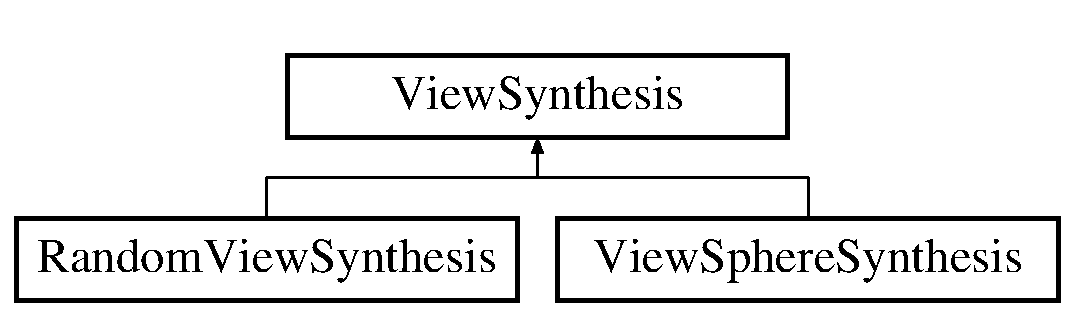
\includegraphics[height=2.000000cm]{classViewSynthesis}
\end{center}
\end{figure}
\subsection*{Public Member Functions}
\begin{DoxyCompactItemize}
\item 
virtual void {\bfseries get\+Views} (\hyperlink{classViewList}{View\+List} \&views)=0\hypertarget{classViewSynthesis_af824834c692508e903544c45c18fd4ed}{}\label{classViewSynthesis_af824834c692508e903544c45c18fd4ed}

\end{DoxyCompactItemize}
\subsection*{Protected Attributes}
\begin{DoxyCompactItemize}
\item 
int {\bfseries n\+\_\+max}\hypertarget{classViewSynthesis_a8afd651580422c328f593cf8e5a6aaf1}{}\label{classViewSynthesis_a8afd651580422c328f593cf8e5a6aaf1}

\end{DoxyCompactItemize}


The documentation for this class was generated from the following files\+:\begin{DoxyCompactItemize}
\item 
partialmodel/viewsynthesis.\+h\item 
partialmodel/viewsynthesis.\+cpp\end{DoxyCompactItemize}

\hypertarget{classvpFileReader}{}\section{vp\+File\+Reader Class Reference}
\label{classvpFileReader}\index{vp\+File\+Reader@{vp\+File\+Reader}}
\subsection*{Public Member Functions}
\begin{DoxyCompactItemize}
\item 
bool \hyperlink{classvpFileReader_acb94e641bcb9efba7155f428a698fe03}{read\+Int} (std\+::string file\+\_\+name, std\+::vector$<$ int $>$ \&data)
\item 
{\footnotesize template$<$typename Tipo $>$ }\\bool {\bfseries read\+Single\+Value} (Tipo \&value, std\+::string file\+\_\+name)\hypertarget{classvpFileReader_afdd319189e19f90738f8597f3634a775}{}\label{classvpFileReader_afdd319189e19f90738f8597f3634a775}

\item 
{\footnotesize template$<$typename Tipo\+Dato $>$ }\\bool {\bfseries read\+M\+S\+L\+Vector} (std\+::vector$<$ Tipo\+Dato $>$ \&data, std\+::string file\+\_\+name)\hypertarget{classvpFileReader_a5d886b245c6339689edd5cdf22d2799f}{}\label{classvpFileReader_a5d886b245c6339689edd5cdf22d2799f}

\item 
{\footnotesize template$<$typename Tipo\+Dato $>$ }\\bool {\bfseries read\+M\+S\+L\+List\+Vector} (std\+::list$<$ std\+::vector$<$ Tipo\+Dato $>$ $>$ \&data, std\+::string file\+\_\+name)\hypertarget{classvpFileReader_a05c2f9d78b751ad28c0683372ca97ace}{}\label{classvpFileReader_a05c2f9d78b751ad28c0683372ca97ace}

\item 
{\footnotesize template$<$typename T $>$ }\\bool \hyperlink{classvpFileReader_a4b4c36bae6e71cb92a7276dfeb96eabc}{save\+To\+M\+S\+L\+List\+Vector} (std\+::list$<$ std\+::vector$<$ T $>$ $>$ data, std\+::string file\+\_\+name, bool append=false)
\item 
{\footnotesize template$<$typename T $>$ }\\bool \hyperlink{classvpFileReader_a805ae83c003da403b40a81a9a7601a82}{save\+Vector\+Of\+Vectors} (std\+::vector$<$ std\+::vector$<$ T $>$ $>$ data, std\+::string file\+\_\+name, bool append=false)
\item 
{\footnotesize template$<$typename T $>$ }\\bool \hyperlink{classvpFileReader_ab02ea430b0fa4bddb69a9e394373f5e8}{save\+List\+Of\+Lists} (std\+::list$<$ std\+::list$<$ T $>$ $>$ data, std\+::string file\+\_\+name, bool append=false)
\item 
{\footnotesize template$<$typename Tipo\+Dato $>$ }\\bool \hyperlink{classvpFileReader_a79619141b6993f7a85fa58acbc72df25}{save\+To\+M\+S\+L\+Vector} (std\+::vector$<$ Tipo\+Dato $>$ \&data, std\+::string file\+\_\+name, bool append=false)
\item 
bool \hyperlink{classvpFileReader_a98aa1278b9e5796d0b7635b34114c46c}{read\+Double} (std\+::string file\+\_\+name, std\+::vector$<$ double $>$ \&data)
\item 
bool {\bfseries read\+Double\+Coord\+From\+P\+CD} (std\+::string file\+\_\+name, std\+::vector$<$ std\+::vector$<$ double $>$ $>$ \&data, std\+::string \&header)\hypertarget{classvpFileReader_a0d77b27e9e96d78453a413adf6c2d88e}{}\label{classvpFileReader_a0d77b27e9e96d78453a413adf6c2d88e}

\item 
bool \hyperlink{classvpFileReader_afc2865630555414a8982e1a9d6baae6e}{read\+Double\+Coordinates} (std\+::string file\+\_\+name, std\+::vector$<$ std\+::vector$<$ double $>$ $>$ \&data)
\item 
bool {\bfseries save\+Double\+Coordinates} (std\+::string file\+\_\+name, std\+::vector$<$ std\+::vector$<$ double $>$ $>$ \&data)\hypertarget{classvpFileReader_a8dd4d28deeb912e483457198ed46bf7f}{}\label{classvpFileReader_a8dd4d28deeb912e483457198ed46bf7f}

\item 
bool {\bfseries read\+Double\+Coordinates\+Coma} (std\+::string file\+\_\+name, std\+::vector$<$ std\+::vector$<$ double $>$ $>$ \&data)\hypertarget{classvpFileReader_af48c0938ba084751d0bc436ae4a6ee85}{}\label{classvpFileReader_af48c0938ba084751d0bc436ae4a6ee85}

\item 
bool {\bfseries read\+Double\+Coordinates\+From\+W\+RL} (std\+::string file\+\_\+name, std\+::vector$<$ std\+::vector$<$ double $>$ $>$ \&data)\hypertarget{classvpFileReader_adfe0b08d6430f9ed55e44fbe8b758f93}{}\label{classvpFileReader_adfe0b08d6430f9ed55e44fbe8b758f93}

\item 
bool {\bfseries save\+Double\+Coordinates\+As\+P\+CD} (std\+::string file\+\_\+name, std\+::vector$<$ std\+::vector$<$ double $>$ $>$ \&data)\hypertarget{classvpFileReader_a71dbfd3ba0f20f2b2225610c70b5fb88}{}\label{classvpFileReader_a71dbfd3ba0f20f2b2225610c70b5fb88}

\item 
bool {\bfseries save\+Double\+Coordinates\+As\+O\+BJ} (std\+::string file\+\_\+name, std\+::vector$<$ std\+::vector$<$ double $>$ $>$ \&data)\hypertarget{classvpFileReader_a297f5cd5f905245c1eab8c506f90ad71}{}\label{classvpFileReader_a297f5cd5f905245c1eab8c506f90ad71}

\item 
{\footnotesize template$<$typename Tipo\+Dato $>$ }\\bool {\bfseries save\+Vector} (std\+::vector$<$ Tipo\+Dato $>$ \&data, std\+::string file\+\_\+name, bool append=false)\hypertarget{classvpFileReader_afcefd226285021787bd622ece9015242}{}\label{classvpFileReader_afcefd226285021787bd622ece9015242}

\item 
{\footnotesize template$<$typename Tipo\+Dato $>$ }\\bool \hyperlink{classvpFileReader_ade854c4030c831c5df01220e3c4b3709}{save\+Data2\+Text} (Tipo\+Dato data, std\+::string file\+\_\+name, bool append=false, char separator= \textquotesingle{} \textquotesingle{})
\end{DoxyCompactItemize}


\subsection{Member Function Documentation}
\index{vp\+File\+Reader@{vp\+File\+Reader}!read\+Double@{read\+Double}}
\index{read\+Double@{read\+Double}!vp\+File\+Reader@{vp\+File\+Reader}}
\subsubsection[{\texorpdfstring{read\+Double(std\+::string file\+\_\+name, std\+::vector$<$ double $>$ \&data)}{readDouble(std::string file_name, std::vector< double > &data)}}]{\setlength{\rightskip}{0pt plus 5cm}bool vp\+File\+Reader\+::read\+Double (
\begin{DoxyParamCaption}
\item[{std\+::string}]{file\+\_\+name, }
\item[{std\+::vector$<$ double $>$ \&}]{data}
\end{DoxyParamCaption}
)}\hypertarget{classvpFileReader_a98aa1278b9e5796d0b7635b34114c46c}{}\label{classvpFileReader_a98aa1278b9e5796d0b7635b34114c46c}
Reads all double numbers from a file \index{vp\+File\+Reader@{vp\+File\+Reader}!read\+Double\+Coordinates@{read\+Double\+Coordinates}}
\index{read\+Double\+Coordinates@{read\+Double\+Coordinates}!vp\+File\+Reader@{vp\+File\+Reader}}
\subsubsection[{\texorpdfstring{read\+Double\+Coordinates(std\+::string file\+\_\+name, std\+::vector$<$ std\+::vector$<$ double $>$ $>$ \&data)}{readDoubleCoordinates(std::string file_name, std::vector< std::vector< double > > &data)}}]{\setlength{\rightskip}{0pt plus 5cm}bool vp\+File\+Reader\+::read\+Double\+Coordinates (
\begin{DoxyParamCaption}
\item[{std\+::string}]{file\+\_\+name, }
\item[{std\+::vector$<$ std\+::vector$<$ double $>$ $>$ \&}]{data}
\end{DoxyParamCaption}
)}\hypertarget{classvpFileReader_afc2865630555414a8982e1a9d6baae6e}{}\label{classvpFileReader_afc2865630555414a8982e1a9d6baae6e}
Reads all double coordinates. \index{vp\+File\+Reader@{vp\+File\+Reader}!read\+Int@{read\+Int}}
\index{read\+Int@{read\+Int}!vp\+File\+Reader@{vp\+File\+Reader}}
\subsubsection[{\texorpdfstring{read\+Int(std\+::string file\+\_\+name, std\+::vector$<$ int $>$ \&data)}{readInt(std::string file_name, std::vector< int > &data)}}]{\setlength{\rightskip}{0pt plus 5cm}bool vp\+File\+Reader\+::read\+Int (
\begin{DoxyParamCaption}
\item[{std\+::string}]{file\+\_\+name, }
\item[{std\+::vector$<$ int $>$ \&}]{data}
\end{DoxyParamCaption}
)}\hypertarget{classvpFileReader_acb94e641bcb9efba7155f428a698fe03}{}\label{classvpFileReader_acb94e641bcb9efba7155f428a698fe03}
Read all int number from a file \index{vp\+File\+Reader@{vp\+File\+Reader}!save\+Data2\+Text@{save\+Data2\+Text}}
\index{save\+Data2\+Text@{save\+Data2\+Text}!vp\+File\+Reader@{vp\+File\+Reader}}
\subsubsection[{\texorpdfstring{save\+Data2\+Text(\+Tipo\+Dato data, std\+::string file\+\_\+name, bool append=false, char separator= \textquotesingle{} \textquotesingle{})}{saveData2Text(TipoDato data, std::string file_name, bool append=false, char separator= ' ')}}]{\setlength{\rightskip}{0pt plus 5cm}template$<$typename Tipo\+Dato $>$ bool vp\+File\+Reader\+::save\+Data2\+Text (
\begin{DoxyParamCaption}
\item[{Tipo\+Dato}]{data, }
\item[{std\+::string}]{file\+\_\+name, }
\item[{bool}]{append = {\ttfamily false}, }
\item[{char}]{separator = {\ttfamily \textquotesingle{}~\textquotesingle{}}}
\end{DoxyParamCaption}
)\hspace{0.3cm}{\ttfamily [inline]}}\hypertarget{classvpFileReader_ade854c4030c831c5df01220e3c4b3709}{}\label{classvpFileReader_ade854c4030c831c5df01220e3c4b3709}
Saves a data to a text file, \index{vp\+File\+Reader@{vp\+File\+Reader}!save\+List\+Of\+Lists@{save\+List\+Of\+Lists}}
\index{save\+List\+Of\+Lists@{save\+List\+Of\+Lists}!vp\+File\+Reader@{vp\+File\+Reader}}
\subsubsection[{\texorpdfstring{save\+List\+Of\+Lists(std\+::list$<$ std\+::list$<$ T $>$ $>$ data, std\+::string file\+\_\+name, bool append=false)}{saveListOfLists(std::list< std::list< T > > data, std::string file_name, bool append=false)}}]{\setlength{\rightskip}{0pt plus 5cm}template$<$typename T $>$ bool vp\+File\+Reader\+::save\+List\+Of\+Lists (
\begin{DoxyParamCaption}
\item[{std\+::list$<$ std\+::list$<$ T $>$ $>$}]{data, }
\item[{std\+::string}]{file\+\_\+name, }
\item[{bool}]{append = {\ttfamily false}}
\end{DoxyParamCaption}
)\hspace{0.3cm}{\ttfamily [inline]}}\hypertarget{classvpFileReader_ab02ea430b0fa4bddb69a9e394373f5e8}{}\label{classvpFileReader_ab02ea430b0fa4bddb69a9e394373f5e8}
Saves a list of lists \index{vp\+File\+Reader@{vp\+File\+Reader}!save\+To\+M\+S\+L\+List\+Vector@{save\+To\+M\+S\+L\+List\+Vector}}
\index{save\+To\+M\+S\+L\+List\+Vector@{save\+To\+M\+S\+L\+List\+Vector}!vp\+File\+Reader@{vp\+File\+Reader}}
\subsubsection[{\texorpdfstring{save\+To\+M\+S\+L\+List\+Vector(std\+::list$<$ std\+::vector$<$ T $>$ $>$ data, std\+::string file\+\_\+name, bool append=false)}{saveToMSLListVector(std::list< std::vector< T > > data, std::string file_name, bool append=false)}}]{\setlength{\rightskip}{0pt plus 5cm}template$<$typename T $>$ bool vp\+File\+Reader\+::save\+To\+M\+S\+L\+List\+Vector (
\begin{DoxyParamCaption}
\item[{std\+::list$<$ std\+::vector$<$ T $>$ $>$}]{data, }
\item[{std\+::string}]{file\+\_\+name, }
\item[{bool}]{append = {\ttfamily false}}
\end{DoxyParamCaption}
)\hspace{0.3cm}{\ttfamily [inline]}}\hypertarget{classvpFileReader_a4b4c36bae6e71cb92a7276dfeb96eabc}{}\label{classvpFileReader_a4b4c36bae6e71cb92a7276dfeb96eabc}
Saves a list of T type vectors in M\+SL format \index{vp\+File\+Reader@{vp\+File\+Reader}!save\+To\+M\+S\+L\+Vector@{save\+To\+M\+S\+L\+Vector}}
\index{save\+To\+M\+S\+L\+Vector@{save\+To\+M\+S\+L\+Vector}!vp\+File\+Reader@{vp\+File\+Reader}}
\subsubsection[{\texorpdfstring{save\+To\+M\+S\+L\+Vector(std\+::vector$<$ Tipo\+Dato $>$ \&data, std\+::string file\+\_\+name, bool append=false)}{saveToMSLVector(std::vector< TipoDato > &data, std::string file_name, bool append=false)}}]{\setlength{\rightskip}{0pt plus 5cm}template$<$typename Tipo\+Dato $>$ bool vp\+File\+Reader\+::save\+To\+M\+S\+L\+Vector (
\begin{DoxyParamCaption}
\item[{std\+::vector$<$ Tipo\+Dato $>$ \&}]{data, }
\item[{std\+::string}]{file\+\_\+name, }
\item[{bool}]{append = {\ttfamily false}}
\end{DoxyParamCaption}
)\hspace{0.3cm}{\ttfamily [inline]}}\hypertarget{classvpFileReader_a79619141b6993f7a85fa58acbc72df25}{}\label{classvpFileReader_a79619141b6993f7a85fa58acbc72df25}
Saves a vector in M\+SL format \index{vp\+File\+Reader@{vp\+File\+Reader}!save\+Vector\+Of\+Vectors@{save\+Vector\+Of\+Vectors}}
\index{save\+Vector\+Of\+Vectors@{save\+Vector\+Of\+Vectors}!vp\+File\+Reader@{vp\+File\+Reader}}
\subsubsection[{\texorpdfstring{save\+Vector\+Of\+Vectors(std\+::vector$<$ std\+::vector$<$ T $>$ $>$ data, std\+::string file\+\_\+name, bool append=false)}{saveVectorOfVectors(std::vector< std::vector< T > > data, std::string file_name, bool append=false)}}]{\setlength{\rightskip}{0pt plus 5cm}template$<$typename T $>$ bool vp\+File\+Reader\+::save\+Vector\+Of\+Vectors (
\begin{DoxyParamCaption}
\item[{std\+::vector$<$ std\+::vector$<$ T $>$ $>$}]{data, }
\item[{std\+::string}]{file\+\_\+name, }
\item[{bool}]{append = {\ttfamily false}}
\end{DoxyParamCaption}
)\hspace{0.3cm}{\ttfamily [inline]}}\hypertarget{classvpFileReader_a805ae83c003da403b40a81a9a7601a82}{}\label{classvpFileReader_a805ae83c003da403b40a81a9a7601a82}
Saves a vector of vectors 

The documentation for this class was generated from the following files\+:\begin{DoxyCompactItemize}
\item 
partialmodel/vpfilereader.\+h\item 
partialmodel/vpfilereader.\+cpp\end{DoxyCompactItemize}

\hypertarget{classvprFreeFlyer}{}\section{vpr\+Free\+Flyer Class Reference}
\label{classvprFreeFlyer}\index{vpr\+Free\+Flyer@{vpr\+Free\+Flyer}}


{\ttfamily \#include $<$vprfreeflyer.\+h$>$}

Inheritance diagram for vpr\+Free\+Flyer\+:\begin{figure}[H]
\begin{center}
\leavevmode
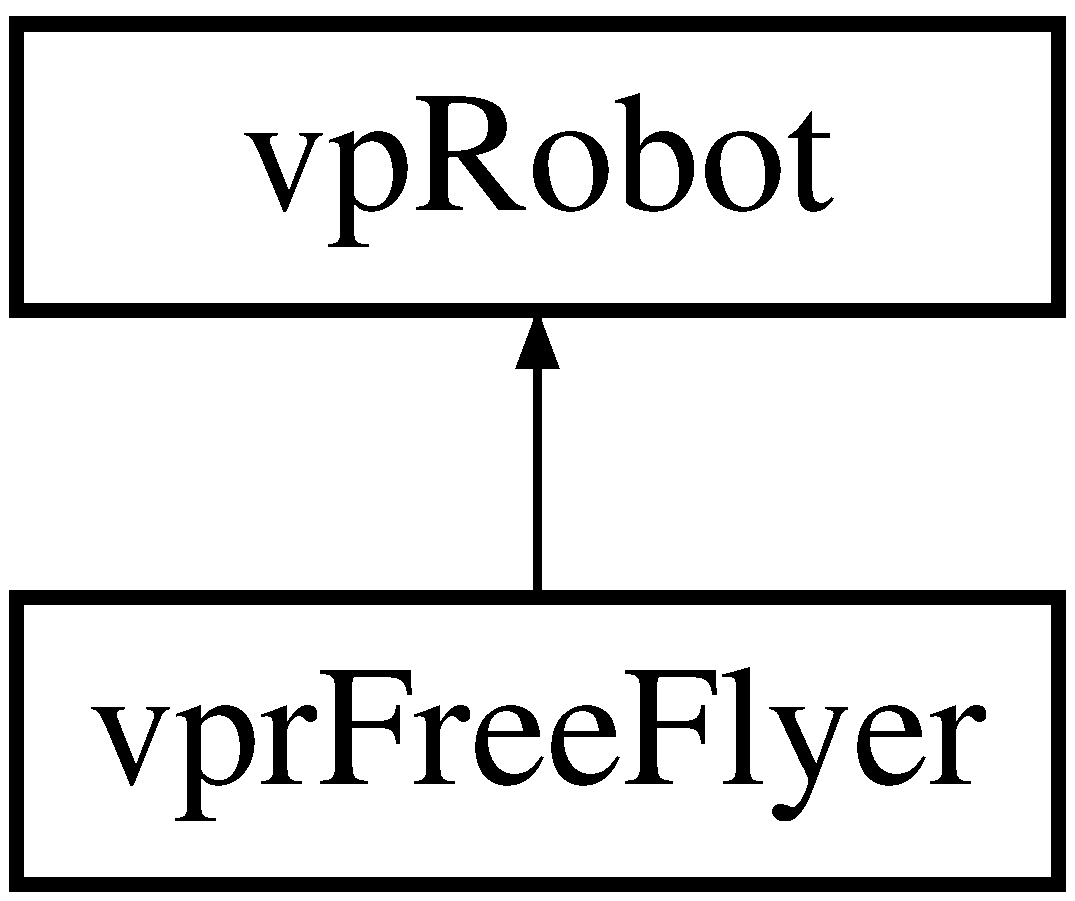
\includegraphics[height=2.000000cm]{classvprFreeFlyer}
\end{center}
\end{figure}
\subsection*{Public Member Functions}
\begin{DoxyCompactItemize}
\item 
virtual void {\bfseries get\+Pose\+From\+Configuration} (mrpt\+::poses\+::\+C\+Pose3D \&pose, std\+::vector$<$ double $>$ q)\hypertarget{classvprFreeFlyer_ab6d24adbcd9c30b464dae8b036468394}{}\label{classvprFreeFlyer_ab6d24adbcd9c30b464dae8b036468394}

\item 
virtual void {\bfseries get\+Current\+H\+TM} (Boost\+Matrix \&H\+TM)\hypertarget{classvprFreeFlyer_ad90b7ba9c7aab39f3b27742fb3e4832d}{}\label{classvprFreeFlyer_ad90b7ba9c7aab39f3b27742fb3e4832d}

\item 
virtual void {\bfseries get\+H\+T\+Mfrom\+Configuration} (Boost\+Matrix \&H\+TM, std\+::vector$<$ double, std\+::allocator$<$ double $>$ $>$ q)\hypertarget{classvprFreeFlyer_a4ddb9bef245d3aec62cf843e29364a52}{}\label{classvprFreeFlyer_a4ddb9bef245d3aec62cf843e29364a52}

\item 
virtual bool {\bfseries move\+To\+Configuration} (std\+::vector$<$ double, std\+::allocator$<$ double $>$ $>$ configuration)\hypertarget{classvprFreeFlyer_a3363bcae45eb475c8785ff2a08f43109}{}\label{classvprFreeFlyer_a3363bcae45eb475c8785ff2a08f43109}

\item 
virtual float {\bfseries execute\+Trajectory} (std\+::vector$<$ std\+::vector$<$ double $>$ $>$ controls, double delta\+\_\+t, std\+::vector$<$ double $>$ goal\+\_\+q)\hypertarget{classvprFreeFlyer_ada428e9717d0e11e892215a4934bfa93}{}\label{classvprFreeFlyer_ada428e9717d0e11e892215a4934bfa93}

\item 
virtual float \hyperlink{classvprFreeFlyer_a8addee690a582bc74577ad79da7f02ba}{execute\+Movement} ()
\item 
virtual void {\bfseries get\+Current\+Configuration} (std\+::vector$<$ double, std\+::allocator$<$ double $>$ $>$ \&q)\hypertarget{classvprFreeFlyer_a17407e2a36c81f754e59ef2619b3f43d}{}\label{classvprFreeFlyer_a17407e2a36c81f754e59ef2619b3f43d}

\item 
virtual bool \hyperlink{classvprFreeFlyer_a9f1f0452b42a29b9cbef9cff075387ce}{set\+Velocities} (std\+::vector$<$ double $>$ velocities)
\item 
virtual bool \hyperlink{classvprFreeFlyer_a28a63f561bd1d740977a1050f10843b1}{init} ()
\item 
void \hyperlink{classvprFreeFlyer_af03adddc180ac01f0a3a49327bd763d1}{generate\+Pointed\+Views} (std\+::list$<$ \hyperlink{classViewStructure}{View\+Structure} $>$ \&view\+List, std\+::string points\+\_\+file, std\+::vector$<$ double $>$ object\+\_\+center, double radio)
\item 
virtual void \hyperlink{classvprFreeFlyer_a65e4457b0c4bb9dbf0eaf9e8cca3daa0}{update\+Robot\+Localization} (mrpt\+::poses\+::\+C\+Pose3D transformation)
\end{DoxyCompactItemize}
\subsection*{Additional Inherited Members}


\subsection{Detailed Description}
A configuration is especified by x, y, z, yaw z, pitch y, roll x all robots work with mm and rads 

\subsection{Member Function Documentation}
\index{vpr\+Free\+Flyer@{vpr\+Free\+Flyer}!execute\+Movement@{execute\+Movement}}
\index{execute\+Movement@{execute\+Movement}!vpr\+Free\+Flyer@{vpr\+Free\+Flyer}}
\subsubsection[{\texorpdfstring{execute\+Movement()}{executeMovement()}}]{\setlength{\rightskip}{0pt plus 5cm}float vpr\+Free\+Flyer\+::execute\+Movement (
\begin{DoxyParamCaption}
{}
\end{DoxyParamCaption}
)\hspace{0.3cm}{\ttfamily [virtual]}}\hypertarget{classvprFreeFlyer_a8addee690a582bc74577ad79da7f02ba}{}\label{classvprFreeFlyer_a8addee690a582bc74577ad79da7f02ba}
Stored movement in trajectory or path. Trajectory of path is executed depending on the robot capabilities Requires a path and a trajectory stablished in path\+To\+Execute and trajectory\+To\+Execute 

Implements \hyperlink{classvpRobot_a7fa1eb51637125595e9a9c46d9b8449f}{vp\+Robot}.

\index{vpr\+Free\+Flyer@{vpr\+Free\+Flyer}!generate\+Pointed\+Views@{generate\+Pointed\+Views}}
\index{generate\+Pointed\+Views@{generate\+Pointed\+Views}!vpr\+Free\+Flyer@{vpr\+Free\+Flyer}}
\subsubsection[{\texorpdfstring{generate\+Pointed\+Views(std\+::list$<$ View\+Structure $>$ \&view\+List, std\+::string points\+\_\+file, std\+::vector$<$ double $>$ object\+\_\+center, double radio)}{generatePointedViews(std::list< ViewStructure > &viewList, std::string points_file, std::vector< double > object_center, double radio)}}]{\setlength{\rightskip}{0pt plus 5cm}void vpr\+Free\+Flyer\+::generate\+Pointed\+Views (
\begin{DoxyParamCaption}
\item[{std\+::list$<$ {\bf View\+Structure} $>$ \&}]{view\+List, }
\item[{std\+::string}]{points\+\_\+file, }
\item[{std\+::vector$<$ double $>$}]{object\+\_\+center, }
\item[{double}]{radio}
\end{DoxyParamCaption}
)}\hypertarget{classvprFreeFlyer_af03adddc180ac01f0a3a49327bd763d1}{}\label{classvprFreeFlyer_af03adddc180ac01f0a3a49327bd763d1}
Generates a set of views which point to a object 
\begin{DoxyParams}{Parameters}
{\em radio} & in mts \\
\hline
\end{DoxyParams}
unit sphere point

view sphere point \index{vpr\+Free\+Flyer@{vpr\+Free\+Flyer}!init@{init}}
\index{init@{init}!vpr\+Free\+Flyer@{vpr\+Free\+Flyer}}
\subsubsection[{\texorpdfstring{init()}{init()}}]{\setlength{\rightskip}{0pt plus 5cm}bool vpr\+Free\+Flyer\+::init (
\begin{DoxyParamCaption}
{}
\end{DoxyParamCaption}
)\hspace{0.3cm}{\ttfamily [virtual]}}\hypertarget{classvprFreeFlyer_a28a63f561bd1d740977a1050f10843b1}{}\label{classvprFreeFlyer_a28a63f561bd1d740977a1050f10843b1}
Initialices the robot, for example the comunication 

Reimplemented from \hyperlink{classvpRobot_a0442d8cd3c8fd883a9df619492b8835f}{vp\+Robot}.

\index{vpr\+Free\+Flyer@{vpr\+Free\+Flyer}!set\+Velocities@{set\+Velocities}}
\index{set\+Velocities@{set\+Velocities}!vpr\+Free\+Flyer@{vpr\+Free\+Flyer}}
\subsubsection[{\texorpdfstring{set\+Velocities(std\+::vector$<$ double $>$ velocities)}{setVelocities(std::vector< double > velocities)}}]{\setlength{\rightskip}{0pt plus 5cm}bool vpr\+Free\+Flyer\+::set\+Velocities (
\begin{DoxyParamCaption}
\item[{std\+::vector$<$ double $>$}]{velocities}
\end{DoxyParamCaption}
)\hspace{0.3cm}{\ttfamily [virtual]}}\hypertarget{classvprFreeFlyer_a9f1f0452b42a29b9cbef9cff075387ce}{}\label{classvprFreeFlyer_a9f1f0452b42a29b9cbef9cff075387ce}
For physical robot 

Implements \hyperlink{classvpRobot_a9c659e2e6f1eb3ed6996885dfb62b8cd}{vp\+Robot}.

\index{vpr\+Free\+Flyer@{vpr\+Free\+Flyer}!update\+Robot\+Localization@{update\+Robot\+Localization}}
\index{update\+Robot\+Localization@{update\+Robot\+Localization}!vpr\+Free\+Flyer@{vpr\+Free\+Flyer}}
\subsubsection[{\texorpdfstring{update\+Robot\+Localization(mrpt\+::poses\+::\+C\+Pose3\+D transformation)}{updateRobotLocalization(mrpt::poses::CPose3D transformation)}}]{\setlength{\rightskip}{0pt plus 5cm}void vpr\+Free\+Flyer\+::update\+Robot\+Localization (
\begin{DoxyParamCaption}
\item[{mrpt\+::poses\+::\+C\+Pose3D}]{transformation}
\end{DoxyParamCaption}
)\hspace{0.3cm}{\ttfamily [virtual]}}\hypertarget{classvprFreeFlyer_a65e4457b0c4bb9dbf0eaf9e8cca3daa0}{}\label{classvprFreeFlyer_a65e4457b0c4bb9dbf0eaf9e8cca3daa0}
Translates the location of the robot 

Implements \hyperlink{classvpRobot_a92d30ca2e923a33e3fb33d5a9c0d3923}{vp\+Robot}.



The documentation for this class was generated from the following files\+:\begin{DoxyCompactItemize}
\item 
viewplanning/vprfreeflyer.\+h\item 
viewplanning/vprfreeflyer.\+cpp\end{DoxyCompactItemize}

\hypertarget{classvpRobot}{}\section{vp\+Robot Class Reference}
\label{classvpRobot}\index{vp\+Robot@{vp\+Robot}}


{\ttfamily \#include $<$vprobot.\+h$>$}

Inheritance diagram for vp\+Robot\+:\begin{figure}[H]
\begin{center}
\leavevmode
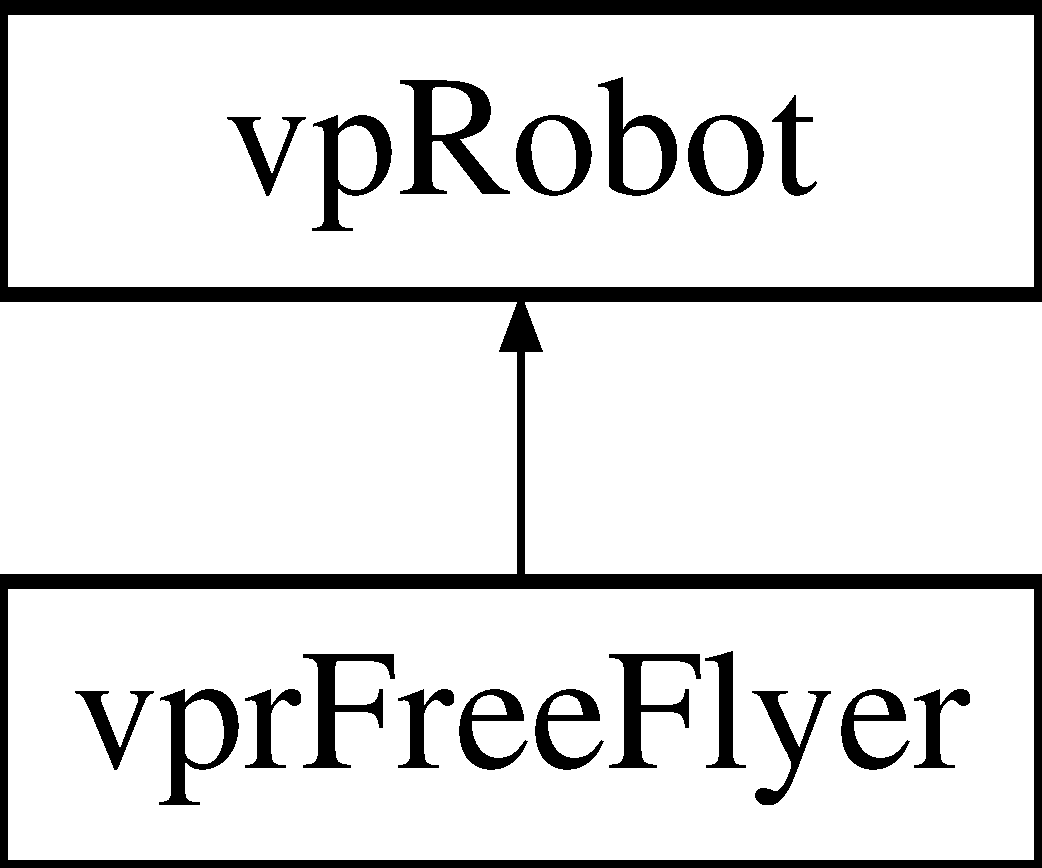
\includegraphics[height=2.000000cm]{classvpRobot}
\end{center}
\end{figure}
\subsection*{Public Member Functions}
\begin{DoxyCompactItemize}
\item 
virtual bool \hyperlink{classvpRobot_a0442d8cd3c8fd883a9df619492b8835f}{init} ()
\item 
virtual void \hyperlink{classvpRobot_a4a234ba83e9c7155f645576775f10804}{get\+Current\+Configuration} (std\+::vector$<$ double $>$ \&q)=0
\item 
virtual bool \hyperlink{classvpRobot_a71bf1d8b8a81feacadf0164d080e87ce}{move\+To\+Configuration} (std\+::vector$<$ double $>$ configuration)=0
\item 
virtual bool \hyperlink{classvpRobot_a9c659e2e6f1eb3ed6996885dfb62b8cd}{set\+Velocities} (std\+::vector$<$ double $>$ velocities)=0
\item 
virtual float {\bfseries execute\+Trajectory} (std\+::vector$<$ std\+::vector$<$ double $>$ $>$ controls, double delta\+\_\+t, std\+::vector$<$ double $>$ goal\+\_\+q)=0\hypertarget{classvpRobot_a2120d527417292e9ddb87619a3446fe2}{}\label{classvpRobot_a2120d527417292e9ddb87619a3446fe2}

\item 
virtual float \hyperlink{classvpRobot_a7fa1eb51637125595e9a9c46d9b8449f}{execute\+Movement} ()=0
\item 
virtual void \hyperlink{classvpRobot_a92d30ca2e923a33e3fb33d5a9c0d3923}{update\+Robot\+Localization} (mrpt\+::poses\+::\+C\+Pose3D transformation)=0
\item 
virtual void \hyperlink{classvpRobot_a9518c5f60297d493673c96c3de1dd247}{get\+H\+T\+Mfrom\+Configuration} (Boost\+Matrix \&H\+TM, std\+::vector$<$ double $>$ q)=0
\item 
virtual void {\bfseries get\+Pose\+From\+Configuration} (mrpt\+::poses\+::\+C\+Pose3D \&pose, std\+::vector$<$ double $>$ q)=0\hypertarget{classvpRobot_add2ab1d988311df8723755b9cf68e5f7}{}\label{classvpRobot_add2ab1d988311df8723755b9cf68e5f7}

\item 
void \hyperlink{classvpRobot_a94cdcc0feed9a2b04eadb996320969d0}{get\+Current\+H\+TM} (Boost\+Matrix \&H\+TM)
\item 
void \hyperlink{classvpRobot_a31725952bb80fd0f0a313cdb2024ea7b}{get\+Current\+Pose} (mrpt\+::poses\+::\+C\+Pose3D \&pose)
\item 
void \hyperlink{classvpRobot_a9b94d096fe152c1b02bde3fb474b7d4a}{get\+Pose\+From\+Configuration} (std\+::vector$<$ double, std\+::allocator$<$ double $>$ $>$ \&pose, std\+::vector$<$ double, std\+::allocator$<$ double $>$ $>$ q)
\item 
void \hyperlink{classvpRobot_a7241b4e2d1d6140adda98735ef2d9be6}{get\+Info} (std\+::string \&inf)
\item 
bool \hyperlink{classvpRobot_a7ff01aeefda9d80e328fe717262721b2}{execute\+Path} ()
\item 
void {\bfseries set\+Config\+Folder} (std\+::string folder)\hypertarget{classvpRobot_a4a20b000e5596904b264835be5b34c2b}{}\label{classvpRobot_a4a20b000e5596904b264835be5b34c2b}

\item 
void {\bfseries set\+Data\+Folder} (std\+::string folder)\hypertarget{classvpRobot_a609cf4359072547554a7c8ff917c5a81}{}\label{classvpRobot_a609cf4359072547554a7c8ff917c5a81}

\item 
void {\bfseries set\+Lower\+State} (std\+::vector$<$ double $>$ state)\hypertarget{classvpRobot_a6495dc7d18d05f226069adf701c03b04}{}\label{classvpRobot_a6495dc7d18d05f226069adf701c03b04}

\item 
void {\bfseries set\+Upper\+State} (std\+::vector$<$ double $>$ state)\hypertarget{classvpRobot_aad26e13564425cd0d128a68d64a84c86}{}\label{classvpRobot_aad26e13564425cd0d128a68d64a84c86}

\item 
void {\bfseries set\+State\+Dim} (int dim)\hypertarget{classvpRobot_a7e00328adf33c213c0a01f2389da1642}{}\label{classvpRobot_a7e00328adf33c213c0a01f2389da1642}

\item 
void \hyperlink{classvpRobot_ae7c97559dac8703c06ec1c8ac75e0878}{get\+Random\+State} (std\+::vector$<$ double $>$ \&state)
\item 
int {\bfseries get\+Config\+Dimension} ()\hypertarget{classvpRobot_a651ceba7e7ac6173688170aa59318806}{}\label{classvpRobot_a651ceba7e7ac6173688170aa59318806}

\item 
int {\bfseries get\+Input\+Dim} ()\hypertarget{classvpRobot_a76e2b6096960dab7bb0dfa9611f621ca}{}\label{classvpRobot_a76e2b6096960dab7bb0dfa9611f621ca}

\end{DoxyCompactItemize}
\subsection*{Public Attributes}
\begin{DoxyCompactItemize}
\item 
std\+::vector$<$ std\+::vector$<$ double $>$ $>$ {\bfseries path\+To\+Execute}\hypertarget{classvpRobot_a62ccc768092b809ae62f2c1a5de3ce77}{}\label{classvpRobot_a62ccc768092b809ae62f2c1a5de3ce77}

\item 
std\+::vector$<$ std\+::vector$<$ double $>$ $>$ {\bfseries trajectory\+To\+Execute}\hypertarget{classvpRobot_ab01511035608dbae618b331627bb62a6}{}\label{classvpRobot_ab01511035608dbae618b331627bb62a6}

\item 
double {\bfseries deltaT}\hypertarget{classvpRobot_a176bd0871646d32657a719d18ad36d50}{}\label{classvpRobot_a176bd0871646d32657a719d18ad36d50}

\item 
std\+::vector$<$ double $>$ {\bfseries goal\+Config}\hypertarget{classvpRobot_a8daac27773e2babc44d295a9f2aa5d81}{}\label{classvpRobot_a8daac27773e2babc44d295a9f2aa5d81}

\end{DoxyCompactItemize}
\subsection*{Protected Attributes}
\begin{DoxyCompactItemize}
\item 
int \hyperlink{classvpRobot_a9dfa07bcea3214993ddcbc50b4d96dde}{configuration\+Dim}\hypertarget{classvpRobot_a9dfa07bcea3214993ddcbc50b4d96dde}{}\label{classvpRobot_a9dfa07bcea3214993ddcbc50b4d96dde}

\begin{DoxyCompactList}\small\item\em Configuration size of the robot. \end{DoxyCompactList}\item 
int \hyperlink{classvpRobot_af0367fab21b8c5b50d6e887805d85169}{state\+Dim}\hypertarget{classvpRobot_af0367fab21b8c5b50d6e887805d85169}{}\label{classvpRobot_af0367fab21b8c5b50d6e887805d85169}

\begin{DoxyCompactList}\small\item\em State Dimension. \end{DoxyCompactList}\item 
int \hyperlink{classvpRobot_abc5e62aa154f90d0556d67b4db577967}{input\+Dim}\hypertarget{classvpRobot_abc5e62aa154f90d0556d67b4db577967}{}\label{classvpRobot_abc5e62aa154f90d0556d67b4db577967}

\begin{DoxyCompactList}\small\item\em input Dimension; \end{DoxyCompactList}\item 
std\+::vector$<$ double $>$ {\bfseries lower\+State}\hypertarget{classvpRobot_a616e0d486e57bd07b5b8d17ee38efcba}{}\label{classvpRobot_a616e0d486e57bd07b5b8d17ee38efcba}

\item 
std\+::vector$<$ double $>$ {\bfseries upper\+State}\hypertarget{classvpRobot_afc811f86ed4da5ce8351601f0b5f2af1}{}\label{classvpRobot_afc811f86ed4da5ce8351601f0b5f2af1}

\item 
std\+::string {\bfseries info}\hypertarget{classvpRobot_a4b3f95d0db1f1d61c89bbcb5e6606780}{}\label{classvpRobot_a4b3f95d0db1f1d61c89bbcb5e6606780}

\item 
bool {\bfseries ready}\hypertarget{classvpRobot_a9be1d7f1a992a63ba5c4b28a610b7bda}{}\label{classvpRobot_a9be1d7f1a992a63ba5c4b28a610b7bda}

\item 
bool {\bfseries verbose}\hypertarget{classvpRobot_a22c4b0445a16700c70c1a18f1f71877e}{}\label{classvpRobot_a22c4b0445a16700c70c1a18f1f71877e}

\item 
std\+::string {\bfseries config\+Folder}\hypertarget{classvpRobot_a8751530956aff9ad1872d447f0452464}{}\label{classvpRobot_a8751530956aff9ad1872d447f0452464}

\item 
std\+::string {\bfseries data\+Folder}\hypertarget{classvpRobot_a7a62d115684aab216717b67f081a8d24}{}\label{classvpRobot_a7a62d115684aab216717b67f081a8d24}

\item 
std\+::string {\bfseries config\+File}\hypertarget{classvpRobot_aa382888b244cc6958ff9ece85eb650b3}{}\label{classvpRobot_aa382888b244cc6958ff9ece85eb650b3}

\end{DoxyCompactItemize}


\subsection{Detailed Description}
Class for the description of a robot. Units\+: mts y radians 

\subsection{Member Function Documentation}
\index{vp\+Robot@{vp\+Robot}!execute\+Movement@{execute\+Movement}}
\index{execute\+Movement@{execute\+Movement}!vp\+Robot@{vp\+Robot}}
\subsubsection[{\texorpdfstring{execute\+Movement()=0}{executeMovement()=0}}]{\setlength{\rightskip}{0pt plus 5cm}virtual float vp\+Robot\+::execute\+Movement (
\begin{DoxyParamCaption}
{}
\end{DoxyParamCaption}
)\hspace{0.3cm}{\ttfamily [pure virtual]}}\hypertarget{classvpRobot_a7fa1eb51637125595e9a9c46d9b8449f}{}\label{classvpRobot_a7fa1eb51637125595e9a9c46d9b8449f}
Stored movement in trajectory or path. Trajectory of path is executed depending on the robot capabilities Requires a path and a trajectory stablished in path\+To\+Execute and trajectory\+To\+Execute 

Implemented in \hyperlink{classvprFreeFlyer_a8addee690a582bc74577ad79da7f02ba}{vpr\+Free\+Flyer}.

\index{vp\+Robot@{vp\+Robot}!execute\+Path@{execute\+Path}}
\index{execute\+Path@{execute\+Path}!vp\+Robot@{vp\+Robot}}
\subsubsection[{\texorpdfstring{execute\+Path()}{executePath()}}]{\setlength{\rightskip}{0pt plus 5cm}bool vp\+Robot\+::execute\+Path (
\begin{DoxyParamCaption}
{}
\end{DoxyParamCaption}
)}\hypertarget{classvpRobot_a7ff01aeefda9d80e328fe717262721b2}{}\label{classvpRobot_a7ff01aeefda9d80e328fe717262721b2}
Calls repeately to move\+To\+Configuration \index{vp\+Robot@{vp\+Robot}!get\+Current\+Configuration@{get\+Current\+Configuration}}
\index{get\+Current\+Configuration@{get\+Current\+Configuration}!vp\+Robot@{vp\+Robot}}
\subsubsection[{\texorpdfstring{get\+Current\+Configuration(std\+::vector$<$ double $>$ \&q)=0}{getCurrentConfiguration(std::vector< double > &q)=0}}]{\setlength{\rightskip}{0pt plus 5cm}virtual void vp\+Robot\+::get\+Current\+Configuration (
\begin{DoxyParamCaption}
\item[{std\+::vector$<$ double $>$ \&}]{q}
\end{DoxyParamCaption}
)\hspace{0.3cm}{\ttfamily [pure virtual]}}\hypertarget{classvpRobot_a4a234ba83e9c7155f645576775f10804}{}\label{classvpRobot_a4a234ba83e9c7155f645576775f10804}


 \subsubsection*{Abstract functions to be implemented in derived classes for physical robot }

Returns the current configuration \index{vp\+Robot@{vp\+Robot}!get\+Current\+H\+TM@{get\+Current\+H\+TM}}
\index{get\+Current\+H\+TM@{get\+Current\+H\+TM}!vp\+Robot@{vp\+Robot}}
\subsubsection[{\texorpdfstring{get\+Current\+H\+T\+M(\+Boost\+Matrix \&\+H\+T\+M)}{getCurrentHTM(BoostMatrix &HTM)}}]{\setlength{\rightskip}{0pt plus 5cm}void vp\+Robot\+::get\+Current\+H\+TM (
\begin{DoxyParamCaption}
\item[{Boost\+Matrix \&}]{H\+TM}
\end{DoxyParamCaption}
)}\hypertarget{classvpRobot_a94cdcc0feed9a2b04eadb996320969d0}{}\label{classvpRobot_a94cdcc0feed9a2b04eadb996320969d0}


 \subsubsection*{--- Generic functions to all derived classes implementations -\/-\/------ }

Gets the transformation matrix for the end effector of the robot. A point seen from the end effector frame reference must be multiplied by this H\+TM 
\begin{DoxyParams}{Parameters}
{\em H\+TM} & \mbox{[}out\mbox{]} Matrix of 4x4 \\
\hline
\end{DoxyParams}
\index{vp\+Robot@{vp\+Robot}!get\+Current\+Pose@{get\+Current\+Pose}}
\index{get\+Current\+Pose@{get\+Current\+Pose}!vp\+Robot@{vp\+Robot}}
\subsubsection[{\texorpdfstring{get\+Current\+Pose(mrpt\+::poses\+::\+C\+Pose3\+D \&pose)}{getCurrentPose(mrpt::poses::CPose3D &pose)}}]{\setlength{\rightskip}{0pt plus 5cm}void vp\+Robot\+::get\+Current\+Pose (
\begin{DoxyParamCaption}
\item[{mrpt\+::poses\+::\+C\+Pose3D \&}]{pose}
\end{DoxyParamCaption}
)}\hypertarget{classvpRobot_a31725952bb80fd0f0a313cdb2024ea7b}{}\label{classvpRobot_a31725952bb80fd0f0a313cdb2024ea7b}
Gets the end effector pose \index{vp\+Robot@{vp\+Robot}!get\+H\+T\+Mfrom\+Configuration@{get\+H\+T\+Mfrom\+Configuration}}
\index{get\+H\+T\+Mfrom\+Configuration@{get\+H\+T\+Mfrom\+Configuration}!vp\+Robot@{vp\+Robot}}
\subsubsection[{\texorpdfstring{get\+H\+T\+Mfrom\+Configuration(\+Boost\+Matrix \&\+H\+T\+M, std\+::vector$<$ double $>$ q)=0}{getHTMfromConfiguration(BoostMatrix &HTM, std::vector< double > q)=0}}]{\setlength{\rightskip}{0pt plus 5cm}virtual void vp\+Robot\+::get\+H\+T\+Mfrom\+Configuration (
\begin{DoxyParamCaption}
\item[{Boost\+Matrix \&}]{H\+TM, }
\item[{std\+::vector$<$ double $>$}]{q}
\end{DoxyParamCaption}
)\hspace{0.3cm}{\ttfamily [pure virtual]}}\hypertarget{classvpRobot_a9518c5f60297d493673c96c3de1dd247}{}\label{classvpRobot_a9518c5f60297d493673c96c3de1dd247}


 \subsubsection*{Model implementations }\index{vp\+Robot@{vp\+Robot}!get\+Info@{get\+Info}}
\index{get\+Info@{get\+Info}!vp\+Robot@{vp\+Robot}}
\subsubsection[{\texorpdfstring{get\+Info(std\+::string \&inf)}{getInfo(std::string &inf)}}]{\setlength{\rightskip}{0pt plus 5cm}void vp\+Robot\+::get\+Info (
\begin{DoxyParamCaption}
\item[{std\+::string \&}]{inf}
\end{DoxyParamCaption}
)}\hypertarget{classvpRobot_a7241b4e2d1d6140adda98735ef2d9be6}{}\label{classvpRobot_a7241b4e2d1d6140adda98735ef2d9be6}
Returns information about the robot \index{vp\+Robot@{vp\+Robot}!get\+Pose\+From\+Configuration@{get\+Pose\+From\+Configuration}}
\index{get\+Pose\+From\+Configuration@{get\+Pose\+From\+Configuration}!vp\+Robot@{vp\+Robot}}
\subsubsection[{\texorpdfstring{get\+Pose\+From\+Configuration(std\+::vector$<$ double, std\+::allocator$<$ double $>$ $>$ \&pose, std\+::vector$<$ double, std\+::allocator$<$ double $>$ $>$ q)}{getPoseFromConfiguration(std::vector< double, std::allocator< double > > &pose, std::vector< double, std::allocator< double > > q)}}]{\setlength{\rightskip}{0pt plus 5cm}void vp\+Robot\+::get\+Pose\+From\+Configuration (
\begin{DoxyParamCaption}
\item[{std\+::vector$<$ double, std\+::allocator$<$ double $>$ $>$ \&}]{pose, }
\item[{std\+::vector$<$ double, std\+::allocator$<$ double $>$ $>$}]{q}
\end{DoxyParamCaption}
)}\hypertarget{classvpRobot_a9b94d096fe152c1b02bde3fb474b7d4a}{}\label{classvpRobot_a9b94d096fe152c1b02bde3fb474b7d4a}
Used for convinience Just call to get\+Pose\+From\+Configuration \index{vp\+Robot@{vp\+Robot}!get\+Random\+State@{get\+Random\+State}}
\index{get\+Random\+State@{get\+Random\+State}!vp\+Robot@{vp\+Robot}}
\subsubsection[{\texorpdfstring{get\+Random\+State(std\+::vector$<$ double $>$ \&state)}{getRandomState(std::vector< double > &state)}}]{\setlength{\rightskip}{0pt plus 5cm}void vp\+Robot\+::get\+Random\+State (
\begin{DoxyParamCaption}
\item[{std\+::vector$<$ double $>$ \&}]{state}
\end{DoxyParamCaption}
)}\hypertarget{classvpRobot_ae7c97559dac8703c06ec1c8ac75e0878}{}\label{classvpRobot_ae7c97559dac8703c06ec1c8ac75e0878}
Gets a random state between lower and upper states \index{vp\+Robot@{vp\+Robot}!init@{init}}
\index{init@{init}!vp\+Robot@{vp\+Robot}}
\subsubsection[{\texorpdfstring{init()}{init()}}]{\setlength{\rightskip}{0pt plus 5cm}bool vp\+Robot\+::init (
\begin{DoxyParamCaption}
{}
\end{DoxyParamCaption}
)\hspace{0.3cm}{\ttfamily [virtual]}}\hypertarget{classvpRobot_a0442d8cd3c8fd883a9df619492b8835f}{}\label{classvpRobot_a0442d8cd3c8fd883a9df619492b8835f}
Initialices the robot, for example the comunication 

Reimplemented in \hyperlink{classvprFreeFlyer_a28a63f561bd1d740977a1050f10843b1}{vpr\+Free\+Flyer}.

\index{vp\+Robot@{vp\+Robot}!move\+To\+Configuration@{move\+To\+Configuration}}
\index{move\+To\+Configuration@{move\+To\+Configuration}!vp\+Robot@{vp\+Robot}}
\subsubsection[{\texorpdfstring{move\+To\+Configuration(std\+::vector$<$ double $>$ configuration)=0}{moveToConfiguration(std::vector< double > configuration)=0}}]{\setlength{\rightskip}{0pt plus 5cm}virtual bool vp\+Robot\+::move\+To\+Configuration (
\begin{DoxyParamCaption}
\item[{std\+::vector$<$ double $>$}]{configuration}
\end{DoxyParamCaption}
)\hspace{0.3cm}{\ttfamily [pure virtual]}}\hypertarget{classvpRobot_a71bf1d8b8a81feacadf0164d080e87ce}{}\label{classvpRobot_a71bf1d8b8a81feacadf0164d080e87ce}
Replaces the current configuration with the given configuration There is no movement T\+O\+DO for all derived classes The robot moves to a configuration. The movement is directly. No collision is checked. The robot moves by its own planning \index{vp\+Robot@{vp\+Robot}!set\+Velocities@{set\+Velocities}}
\index{set\+Velocities@{set\+Velocities}!vp\+Robot@{vp\+Robot}}
\subsubsection[{\texorpdfstring{set\+Velocities(std\+::vector$<$ double $>$ velocities)=0}{setVelocities(std::vector< double > velocities)=0}}]{\setlength{\rightskip}{0pt plus 5cm}virtual bool vp\+Robot\+::set\+Velocities (
\begin{DoxyParamCaption}
\item[{std\+::vector$<$ double $>$}]{velocities}
\end{DoxyParamCaption}
)\hspace{0.3cm}{\ttfamily [pure virtual]}}\hypertarget{classvpRobot_a9c659e2e6f1eb3ed6996885dfb62b8cd}{}\label{classvpRobot_a9c659e2e6f1eb3ed6996885dfb62b8cd}
For physical robot 

Implemented in \hyperlink{classvprFreeFlyer_a9f1f0452b42a29b9cbef9cff075387ce}{vpr\+Free\+Flyer}.

\index{vp\+Robot@{vp\+Robot}!update\+Robot\+Localization@{update\+Robot\+Localization}}
\index{update\+Robot\+Localization@{update\+Robot\+Localization}!vp\+Robot@{vp\+Robot}}
\subsubsection[{\texorpdfstring{update\+Robot\+Localization(mrpt\+::poses\+::\+C\+Pose3\+D transformation)=0}{updateRobotLocalization(mrpt::poses::CPose3D transformation)=0}}]{\setlength{\rightskip}{0pt plus 5cm}virtual void vp\+Robot\+::update\+Robot\+Localization (
\begin{DoxyParamCaption}
\item[{mrpt\+::poses\+::\+C\+Pose3D}]{transformation}
\end{DoxyParamCaption}
)\hspace{0.3cm}{\ttfamily [pure virtual]}}\hypertarget{classvpRobot_a92d30ca2e923a33e3fb33d5a9c0d3923}{}\label{classvpRobot_a92d30ca2e923a33e3fb33d5a9c0d3923}
Translates the location of the robot 

Implemented in \hyperlink{classvprFreeFlyer_a65e4457b0c4bb9dbf0eaf9e8cca3daa0}{vpr\+Free\+Flyer}.



The documentation for this class was generated from the following files\+:\begin{DoxyCompactItemize}
\item 
viewplanning/vprobot.\+h\item 
viewplanning/vprobot.\+cpp\end{DoxyCompactItemize}

\hypertarget{classvpTriangle}{}\section{vp\+Triangle Class Reference}
\label{classvpTriangle}\index{vp\+Triangle@{vp\+Triangle}}
\subsection*{Public Member Functions}
\begin{DoxyCompactItemize}
\item 
{\bfseries vp\+Triangle} (\hyperlink{classvpVertex}{vp\+Vertex} v1, \hyperlink{classvpVertex}{vp\+Vertex} v2, \hyperlink{classvpVertex}{vp\+Vertex} v3)\hypertarget{classvpTriangle_afcf460b224661ae457af66dc8ead5926}{}\label{classvpTriangle_afcf460b224661ae457af66dc8ead5926}

\end{DoxyCompactItemize}
\subsection*{Public Attributes}
\begin{DoxyCompactItemize}
\item 
\hyperlink{classvpVertex}{vp\+Vertex} {\bfseries a}\hypertarget{classvpTriangle_a83917be37c07ba8368a313c2bfb9d346}{}\label{classvpTriangle_a83917be37c07ba8368a313c2bfb9d346}

\item 
\hyperlink{classvpVertex}{vp\+Vertex} {\bfseries b}\hypertarget{classvpTriangle_afe5486a0daf3bd954c98ac6a894c46ec}{}\label{classvpTriangle_afe5486a0daf3bd954c98ac6a894c46ec}

\item 
\hyperlink{classvpVertex}{vp\+Vertex} {\bfseries c}\hypertarget{classvpTriangle_a4fbff84da01f97fd84abf3b73bc2f25e}{}\label{classvpTriangle_a4fbff84da01f97fd84abf3b73bc2f25e}

\end{DoxyCompactItemize}


The documentation for this class was generated from the following files\+:\begin{DoxyCompactItemize}
\item 
partialmodel/vptriangle.\+h\item 
partialmodel/vptriangle.\+cpp\end{DoxyCompactItemize}

\hypertarget{classvpTriangleList}{}\section{vp\+Triangle\+List Class Reference}
\label{classvpTriangleList}\index{vp\+Triangle\+List@{vp\+Triangle\+List}}
Inheritance diagram for vp\+Triangle\+List\+:\begin{figure}[H]
\begin{center}
\leavevmode
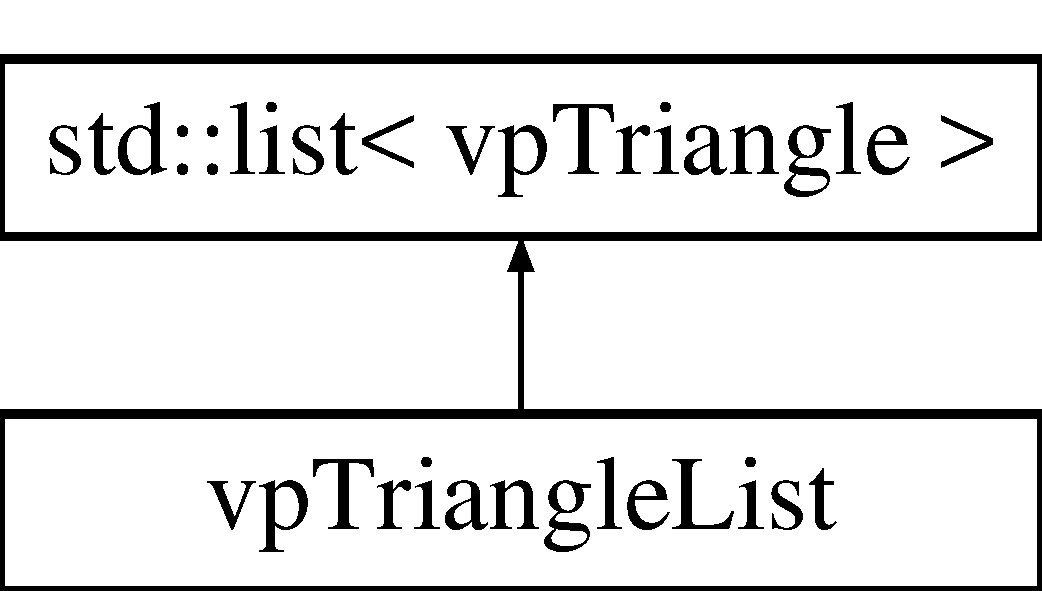
\includegraphics[height=2.000000cm]{classvpTriangleList}
\end{center}
\end{figure}
\subsection*{Public Member Functions}
\begin{DoxyCompactItemize}
\item 
bool \hyperlink{classvpTriangleList_a07dec3a121cfb0119f2fcca6f36cb4a1}{save\+To\+File} (std\+::string file\+\_\+name)
\item 
bool {\bfseries save\+To\+M\+S\+L\+Triangle} (std\+::string file\+\_\+name)\hypertarget{classvpTriangleList_aabff182774adb08821ca2a67fe9e37e3}{}\label{classvpTriangleList_aabff182774adb08821ca2a67fe9e37e3}

\item 
bool \hyperlink{classvpTriangleList_a174b1ad55190c08fa4381cdf40efab7d}{read\+File} (std\+::string file\+\_\+name)
\end{DoxyCompactItemize}


\subsection{Member Function Documentation}
\index{vp\+Triangle\+List@{vp\+Triangle\+List}!read\+File@{read\+File}}
\index{read\+File@{read\+File}!vp\+Triangle\+List@{vp\+Triangle\+List}}
\subsubsection[{\texorpdfstring{read\+File(std\+::string file\+\_\+name)}{readFile(std::string file_name)}}]{\setlength{\rightskip}{0pt plus 5cm}bool vp\+Triangle\+List\+::read\+File (
\begin{DoxyParamCaption}
\item[{std\+::string}]{file\+\_\+name}
\end{DoxyParamCaption}
)}\hypertarget{classvpTriangleList_a174b1ad55190c08fa4381cdf40efab7d}{}\label{classvpTriangleList_a174b1ad55190c08fa4381cdf40efab7d}
Reads a raw triangle file \index{vp\+Triangle\+List@{vp\+Triangle\+List}!save\+To\+File@{save\+To\+File}}
\index{save\+To\+File@{save\+To\+File}!vp\+Triangle\+List@{vp\+Triangle\+List}}
\subsubsection[{\texorpdfstring{save\+To\+File(std\+::string file\+\_\+name)}{saveToFile(std::string file_name)}}]{\setlength{\rightskip}{0pt plus 5cm}bool vp\+Triangle\+List\+::save\+To\+File (
\begin{DoxyParamCaption}
\item[{std\+::string}]{file\+\_\+name}
\end{DoxyParamCaption}
)}\hypertarget{classvpTriangleList_a07dec3a121cfb0119f2fcca6f36cb4a1}{}\label{classvpTriangleList_a07dec3a121cfb0119f2fcca6f36cb4a1}
Save to raw File 

The documentation for this class was generated from the following files\+:\begin{DoxyCompactItemize}
\item 
partialmodel/vptriangle.\+h\item 
partialmodel/vptriangle.\+cpp\end{DoxyCompactItemize}

\hypertarget{classvpVertex}{}\section{vp\+Vertex Class Reference}
\label{classvpVertex}\index{vp\+Vertex@{vp\+Vertex}}
\subsection*{Public Member Functions}
\begin{DoxyCompactItemize}
\item 
{\bfseries vp\+Vertex} (double coord\+\_\+x, double coord\+\_\+y, double coord\+\_\+z)\hypertarget{classvpVertex_a627586989faad3a010933fe0244771f1}{}\label{classvpVertex_a627586989faad3a010933fe0244771f1}

\item 
void {\bfseries set\+Coordinates} (double coord\+\_\+x, double coord\+\_\+y, double coord\+\_\+z)\hypertarget{classvpVertex_af17a837d95bb5c85fdc8e914c5811b10}{}\label{classvpVertex_af17a837d95bb5c85fdc8e914c5811b10}

\end{DoxyCompactItemize}
\subsection*{Public Attributes}
\begin{DoxyCompactItemize}
\item 
double {\bfseries x}\hypertarget{classvpVertex_af77df39a5035202e8b2dd9b06dbca67a}{}\label{classvpVertex_af77df39a5035202e8b2dd9b06dbca67a}

\item 
double {\bfseries y}\hypertarget{classvpVertex_ac5f67bd42f9d4206e8231d6e0e4ea780}{}\label{classvpVertex_ac5f67bd42f9d4206e8231d6e0e4ea780}

\item 
double {\bfseries z}\hypertarget{classvpVertex_ae06974327c60b5c733daf89a4d1ff4a0}{}\label{classvpVertex_ae06974327c60b5c733daf89a4d1ff4a0}

\end{DoxyCompactItemize}


The documentation for this class was generated from the following files\+:\begin{DoxyCompactItemize}
\item 
partialmodel/vpvertex.\+h\item 
partialmodel/vpvertex.\+cpp\end{DoxyCompactItemize}

\hypertarget{classWorkspaceNBVPlanner}{}\section{Workspace\+N\+B\+V\+Planner Class Reference}
\label{classWorkspaceNBVPlanner}\index{Workspace\+N\+B\+V\+Planner@{Workspace\+N\+B\+V\+Planner}}


{\ttfamily \#include $<$workspacenbvplanner.\+h$>$}

Inheritance diagram for Workspace\+N\+B\+V\+Planner\+:\begin{figure}[H]
\begin{center}
\leavevmode
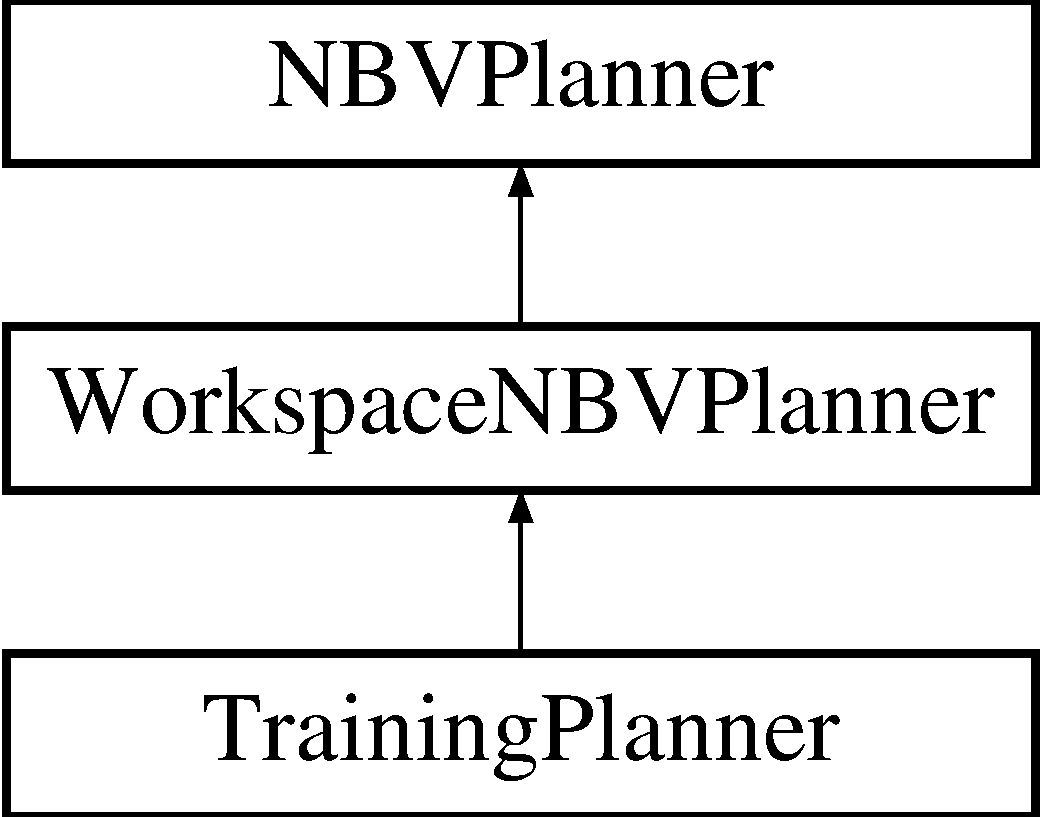
\includegraphics[height=2.000000cm]{classWorkspaceNBVPlanner}
\end{center}
\end{figure}
\subsection*{Public Member Functions}
\begin{DoxyCompactItemize}
\item 
{\bfseries Workspace\+N\+B\+V\+Planner} (\hyperlink{classRobotSensor}{Robot\+Sensor} $\ast$rs, \hyperlink{classPartialModelBase}{Partial\+Model\+Base} $\ast$pm)\hypertarget{classWorkspaceNBVPlanner_a8b29a06fc054a2bb59314b1a8b501068}{}\label{classWorkspaceNBVPlanner_a8b29a06fc054a2bb59314b1a8b501068}

\item 
virtual bool \hyperlink{classWorkspaceNBVPlanner_ad5655e5c1c45a017d4c598fd2632ed49}{plan\+N\+BV} (\hyperlink{classViewStructure}{View\+Structure} \&v)
\item 
virtual bool {\bfseries init} ()\hypertarget{classWorkspaceNBVPlanner_a8fc044565494abfd67a36c4565ca507d}{}\label{classWorkspaceNBVPlanner_a8fc044565494abfd67a36c4565ca507d}

\end{DoxyCompactItemize}
\subsection*{Protected Attributes}
\begin{DoxyCompactItemize}
\item 
std\+::string {\bfseries view\+Sphere\+File\+Name}\hypertarget{classWorkspaceNBVPlanner_aff8df8d09551a89635a5f39c2089ce29}{}\label{classWorkspaceNBVPlanner_aff8df8d09551a89635a5f39c2089ce29}

\item 
std\+::string {\bfseries evaluated\+Views\+File}\hypertarget{classWorkspaceNBVPlanner_a5dd5347db8708cbd72a2bc81d26de9d7}{}\label{classWorkspaceNBVPlanner_a5dd5347db8708cbd72a2bc81d26de9d7}

\item 
\hyperlink{classViewList}{View\+List} {\bfseries candidate\+Views}\hypertarget{classWorkspaceNBVPlanner_ad96bc939d0cb7cefa707d98f51de8e76}{}\label{classWorkspaceNBVPlanner_ad96bc939d0cb7cefa707d98f51de8e76}

\item 
std\+::vector$<$ double $>$ {\bfseries object\+Center}\hypertarget{classWorkspaceNBVPlanner_ad5372c462051e5757370d1fc4682a9e6}{}\label{classWorkspaceNBVPlanner_ad5372c462051e5757370d1fc4682a9e6}

\item 
double {\bfseries radio}\hypertarget{classWorkspaceNBVPlanner_a12a867beffb670bbb574967782727564}{}\label{classWorkspaceNBVPlanner_a12a867beffb670bbb574967782727564}

\end{DoxyCompactItemize}
\subsection*{Additional Inherited Members}


\subsection{Detailed Description}
Planner that computes the N\+BV as a pose (x,y,z,yaw,pitch,roll) In particular, this implemented object generates a view sphere and selects the N\+BV as the view with the highest evaluation depending on the partial model selected

At initialization\+: It generates a view sphere assuming a freeflyer robot which is pointing to the x axis and z is upward The view sphere is taken as configurations of the robot, then It asks to the robot to return the end effector pose and H\+TM The list of candidate\+Views is created

For N\+BV computation\+: It queries to the partial model to evaluate the pointed views 

\subsection{Member Function Documentation}
\index{Workspace\+N\+B\+V\+Planner@{Workspace\+N\+B\+V\+Planner}!plan\+N\+BV@{plan\+N\+BV}}
\index{plan\+N\+BV@{plan\+N\+BV}!Workspace\+N\+B\+V\+Planner@{Workspace\+N\+B\+V\+Planner}}
\subsubsection[{\texorpdfstring{plan\+N\+B\+V(\+View\+Structure \&v)}{planNBV(ViewStructure &v)}}]{\setlength{\rightskip}{0pt plus 5cm}bool Workspace\+N\+B\+V\+Planner\+::plan\+N\+BV (
\begin{DoxyParamCaption}
\item[{{\bf View\+Structure} \&}]{v}
\end{DoxyParamCaption}
)\hspace{0.3cm}{\ttfamily [virtual]}}\hypertarget{classWorkspaceNBVPlanner_ad5655e5c1c45a017d4c598fd2632ed49}{}\label{classWorkspaceNBVPlanner_ad5655e5c1c45a017d4c598fd2632ed49}
Main function, it computes the N\+BV 

Implements \hyperlink{classNBVPlanner_a448567c9d5cec319c5df5efdb0d5479c}{N\+B\+V\+Planner}.



The documentation for this class was generated from the following files\+:\begin{DoxyCompactItemize}
\item 
viewplanning/workspacenbvplanner.\+h\item 
viewplanning/workspacenbvplanner.\+cpp\end{DoxyCompactItemize}

%--- End generated contents ---

% Index
\backmatter
\newpage
\phantomsection
\clearemptydoublepage
\addcontentsline{toc}{chapter}{Index}
\printindex

\end{document}
